\documentclass[12pt,a4paper,twoside]{article} % 2 cares, A4 i a 12 punts
% --------------------------------
%
% PREÁMBULO
%
% --------------------------------

\usepackage[utf8]{inputenc}
\usepackage[T1]{fontenc} % font encode (acentos y tal)
\usepackage[spanish]{babel} % idioma
\usepackage{amsmath} % Simbolos basicos del lenguaje matematico
\usepackage{enumerate} % Para definir facil del tipo de enum
\usepackage{graphicx} % \includegraphics
\usepackage{color,soul} % \hl
\usepackage{amssymb} % \mathbb
\usepackage{amsthm} % Proof environment
\usepackage{placeins} % Para que las figuras salgan donde las pongo
\usepackage[all]{xy} % Para diagramas de morfismos
\usepackage{listings} % Para escribir código
\usepackage{bm} % Para negrita en math mode
\usepackage{fancyhdr} % Capçaleres i peus
\usepackage{mathpazo} % Palatino font
\usepackage{tocloft} % table of contents things

\pagestyle{fancy}
\fancyhf{}
\addtolength{\headheight}{\baselineskip}
\renewcommand{\sectionmark}[1]{\markboth{#1}{}}
\renewcommand{\subsectionmark}[1]{\markright{#1}}
\rhead{\leftmark\\\rightmark}
\fancyhead[RE]{Filtraciones mediante KDE's en homología persistente}
\fancyhead[LO]{\leftmark}
\fancyhead[RO]{\textit{\rightmark}}
\fancyfoot[LE,RO]{\thepage}
\tocloftpagestyle{empty}

\theoremstyle{plain}
\newtheorem{proposicion}{Proposición}[subsection]
\newtheorem{lema}{Lema}[subsection]
\newtheorem{teorema}{Teorema}[subsection]
\newtheorem{corolario}{Corolario}[subsection]
\theoremstyle{definition}
\newtheorem{definicion}{Definición}[subsection]
\newtheorem*{notacion}{Notación}
\newtheorem{observacion}{Observación}[subsection]
\newtheorem{ejemplo}{Ejemplo}[subsection]

\newcommand{\Z}{\mathbb{Z}}
\newcommand{\N}{\mathbb{N}}
\newcommand{\C}{\mathbb{C}}
\newcommand{\R}{\mathbb{R}}
\newcommand{\F}{\mathbb{F}}
\newcommand{\RP}{\mathbb{R}\textup{P}}
\newcommand{\Hn}{H_n(S^n)}
\newcommand{\Nrv}{\mathrm{Nrv}}
\newcommand{\NrvU}{\mathrm{Nrv}\mathcal{U}}
\newcommand{\tq}{\; | \;}
\newcommand{\geom}[1]{\lvert #1 \rvert}
\newcommand{\U}{\mathcal{U}}
\newcommand{\map}[3]{#1 \colon #2 \to #3}
\newcommand{\Img}[1]{\mathrm{Im}#1}
\newcommand{\Map}[5]{\begin{align*}
					#1\colon   #2 &\to     #3 \\
							   #4 &\mapsto #5
					\end{align*}}
\newcommand{\quotient}[2]{{\raisebox{.2em}{$#1$}\left/\raisebox{-.2em}{$#2$}\right.}}
\newcommand*\NewPage{\newpage\null\thispagestyle{empty}\newpage}

\begin{document}
\title{Filtraciones en homología persistente mediante estimadores kernel de densidad}
\author{Martín Campos Heredia}
\begin{titlepage}

%----------------------------------------------------------------------------------------
%
%	TITLE PAGE
%
%----------------------------------------------------------------------------------------


	\newcommand{\HRule}{\rule{\linewidth}{0.5mm}} % Defines a new command for horizontal lines, change thickness here
	
	\center % Centre everything on the page
	
	%------------------------------------------------
	%	Headings
	%------------------------------------------------

	
	\textsc{\large Grado en Matemáticas}\\[0.5cm] % Major heading such as course name
	
	\textsc{Trabajo de Fin de Grado}\\[0.5cm] % Minor heading such as course title
	
	%------------------------------------------------
	%	Title
	%------------------------------------------------
	
	\HRule\\[0.4cm]
	
	{\Large\bfseries Filtraciones en homología persistente mediante estimadores kernel de densidad}\\[0.4cm] % Title of your document

	\HRule\\[1.5cm]
	
	%------------------------------------------------
	%	Author(s)
	%------------------------------------------------
	
	\begin{minipage}{0.4\textwidth}
		\begin{flushleft}
			\large
			\textit{Autor}\\
			Martín H. \textsc{Campos} % Your name
		\end{flushleft}
	\end{minipage}
	~
	\begin{minipage}{0.4\textwidth}
		\begin{flushright}
			\large
			\textit{Supervisor}\\
			Dr. Albert \textsc{Ruiz} % Supervisor's name
		\end{flushright}
	\end{minipage}
	

	% If you don't want a supervisor, uncomment the two lines below and comment the code above
	%{\large\textit{Author}}\\
	%John \textsc{Smith} % Your name

	%------------------------------------------------
	%	Logo
	%------------------------------------------------
	
	\vfill\vfill
    
\includegraphics[scale=0.3]{img/uabnegro.png} % Include a department/university logo - this will require the graphicx package
%	\textsc{\Large Universitat Autònoma de Barcelona}\\[1.5cm] % Main heading such as the name of your university/college
	 
	
	%------------------------------------------------
	%	Date
	%------------------------------------------------
	
	\vfill\vfill % Position the date 3/4 down the remaining page
	
	{\large Junio de 2018} % Date, change the \today to a set date if you want to be precise
	
	%----------------------------------------------------------------------------------------
	
	\vfill % Push the date up 1/4 of the remaining page
	
\end{titlepage}
\NewPage
\tableofcontents
\NewPage

\newpage
\cleardoublepage
\setcounter{page}{1}
\section{Introducción}

% --------------------------------
%
% SECCIÓN 1: INTRODUCCIÓN
%
% --------------------------------

Vivimos en una época donde nos es más fácil obtener datos que procesarlos. Son muchísimas las técnicas que se han desarrollado de un tiempo a esta parte para tratar de sacar la máxima información de toda esa masa informe que los técnicos llaman \emph{Big Data}. En este contexto, el análisis topológico de datos ha crecido con mucha fuerza en los últimos años intentando dar respuesta a la pregunta ``\emph{¿Qué forma tienen los datos?}''.

Una de las ramas que se ha consagrado en la última década es la Homología Persistente, una aplicación de la topología algebraica que estima los grupos de homología de la figura que subyace de una nube de datos. Esencialmente, la Homología Persistente consiste en crear \emph{filtraciones}, que son una colección de objetos que representan la figura subyacente, a partir de los datos. Para construir dichas filtraciones, se utilizan los llamados complejos de Čech o los complejos de Vietoris-Rips (más comunmente los segundos). La principal limitación con la que topa la Homología Persistente es en términos computacionales, ya que el número de elementos de la filtración crece exponencialmente con el número de puntos de la nube de datos a tratar, y esto se vuelve un impedimento a corta escala.

En este trabajo se expone un método alternativo para generar filtraciones mediante el uso de un estimador kernel de densidad (\emph{Kernel Density Estimator, KDE}) de la nube de datos. El tamaño de este tipo de filtraciones no depende del número de puntos, sino de la precisión con la que uno elija trabajar, y de hecho gana robustez frente a ruidos conforme aumente la cantidad de éstos. Este método ha sido implementado con éxito en un módulo de Python que está disponible en los respositorios de PyPI para ser utilizado o mejorado por todo el que lo desee.

Para fabricar este tipo de filtraciones utilizamos un tipo de construcción similar a la de complejo simplicial, pero que utiliza $m$-cubos en vez de $m$-tetraedros. En la Sección 3 se desarrolla formalmente el concepto de grupos de homología sobre este tipo de construcciones, que finalmente vemos que son equivalentes a los del subespacio de $\R^n$ que ocupan. Esta sección contiene la parte de teoría más importante del trabajo y es sobre la que se sostiene todo lo que se ha desarrollado.

En la Sección 2 hacemos un breve repaso de los conceptos básicos de la Homología Persistente y las filtraciones utilizadas a día de hoy. En la Sección 4 se expone formalmente en qué consiste una filtración mediante KDE, utilizando los conceptos definidos en la Sección 3. Por último, en la Sección 5 hablamos del software que se ha desarrollado para implementar dicho método.

\newpage
\NewPage
\section{Homología persistente}

% --------------------------------
%
% SECCIÓN 2: HOMOLOGÍA PERSISTENTE
%
% --------------------------------

La topología algebraica aporta herramientas para calcular los grupos de homología de un espacio topológico. Estos grupos, pese a no ser suficientes para determinar unívocamente el tipo de homotopía, sí son invariantes (por homotopía) y resultan una herramienta muy útil para clasificar. Una buena introducción a la topología algebraica y definición y cálculo de grupos de homología se pueden encontrar en \cite{Navarro} y \cite{Hatcher}.

La homología persistente tiene como objetivo estimar los grupos de homología de la forma que subyace de una nube de datos. Supóngase que se tiene un conjunto finito de $N$ puntos $S \subset\R^n$ del cual se desea conocer la \emph{forma}.

De entrada, el conjunto $S$ en sí no es más que la unión disconexa de $N$ puntos, y por tanto tiene siempre grupos de homología $H_0=R^N$ y $H_i=0$ $\forall i > 0$ sobre cualquier anillo $R$, lo cual no nos aporta absolutamente nada de información para nuestro cometido. En la homología persistente debemos construir espacios que, de una forma u otra, representen la figura subyacente de nuestra nube de datos, y de los cuales los grupos de homología tengan algo que decir. Una primera idea \emph{naif} consiste en reemplazar los puntos por bolas de un cierto radio $r$ que den una forma \emph{más conexa} al conjunto.

\begin{figure}[h!]
\centering
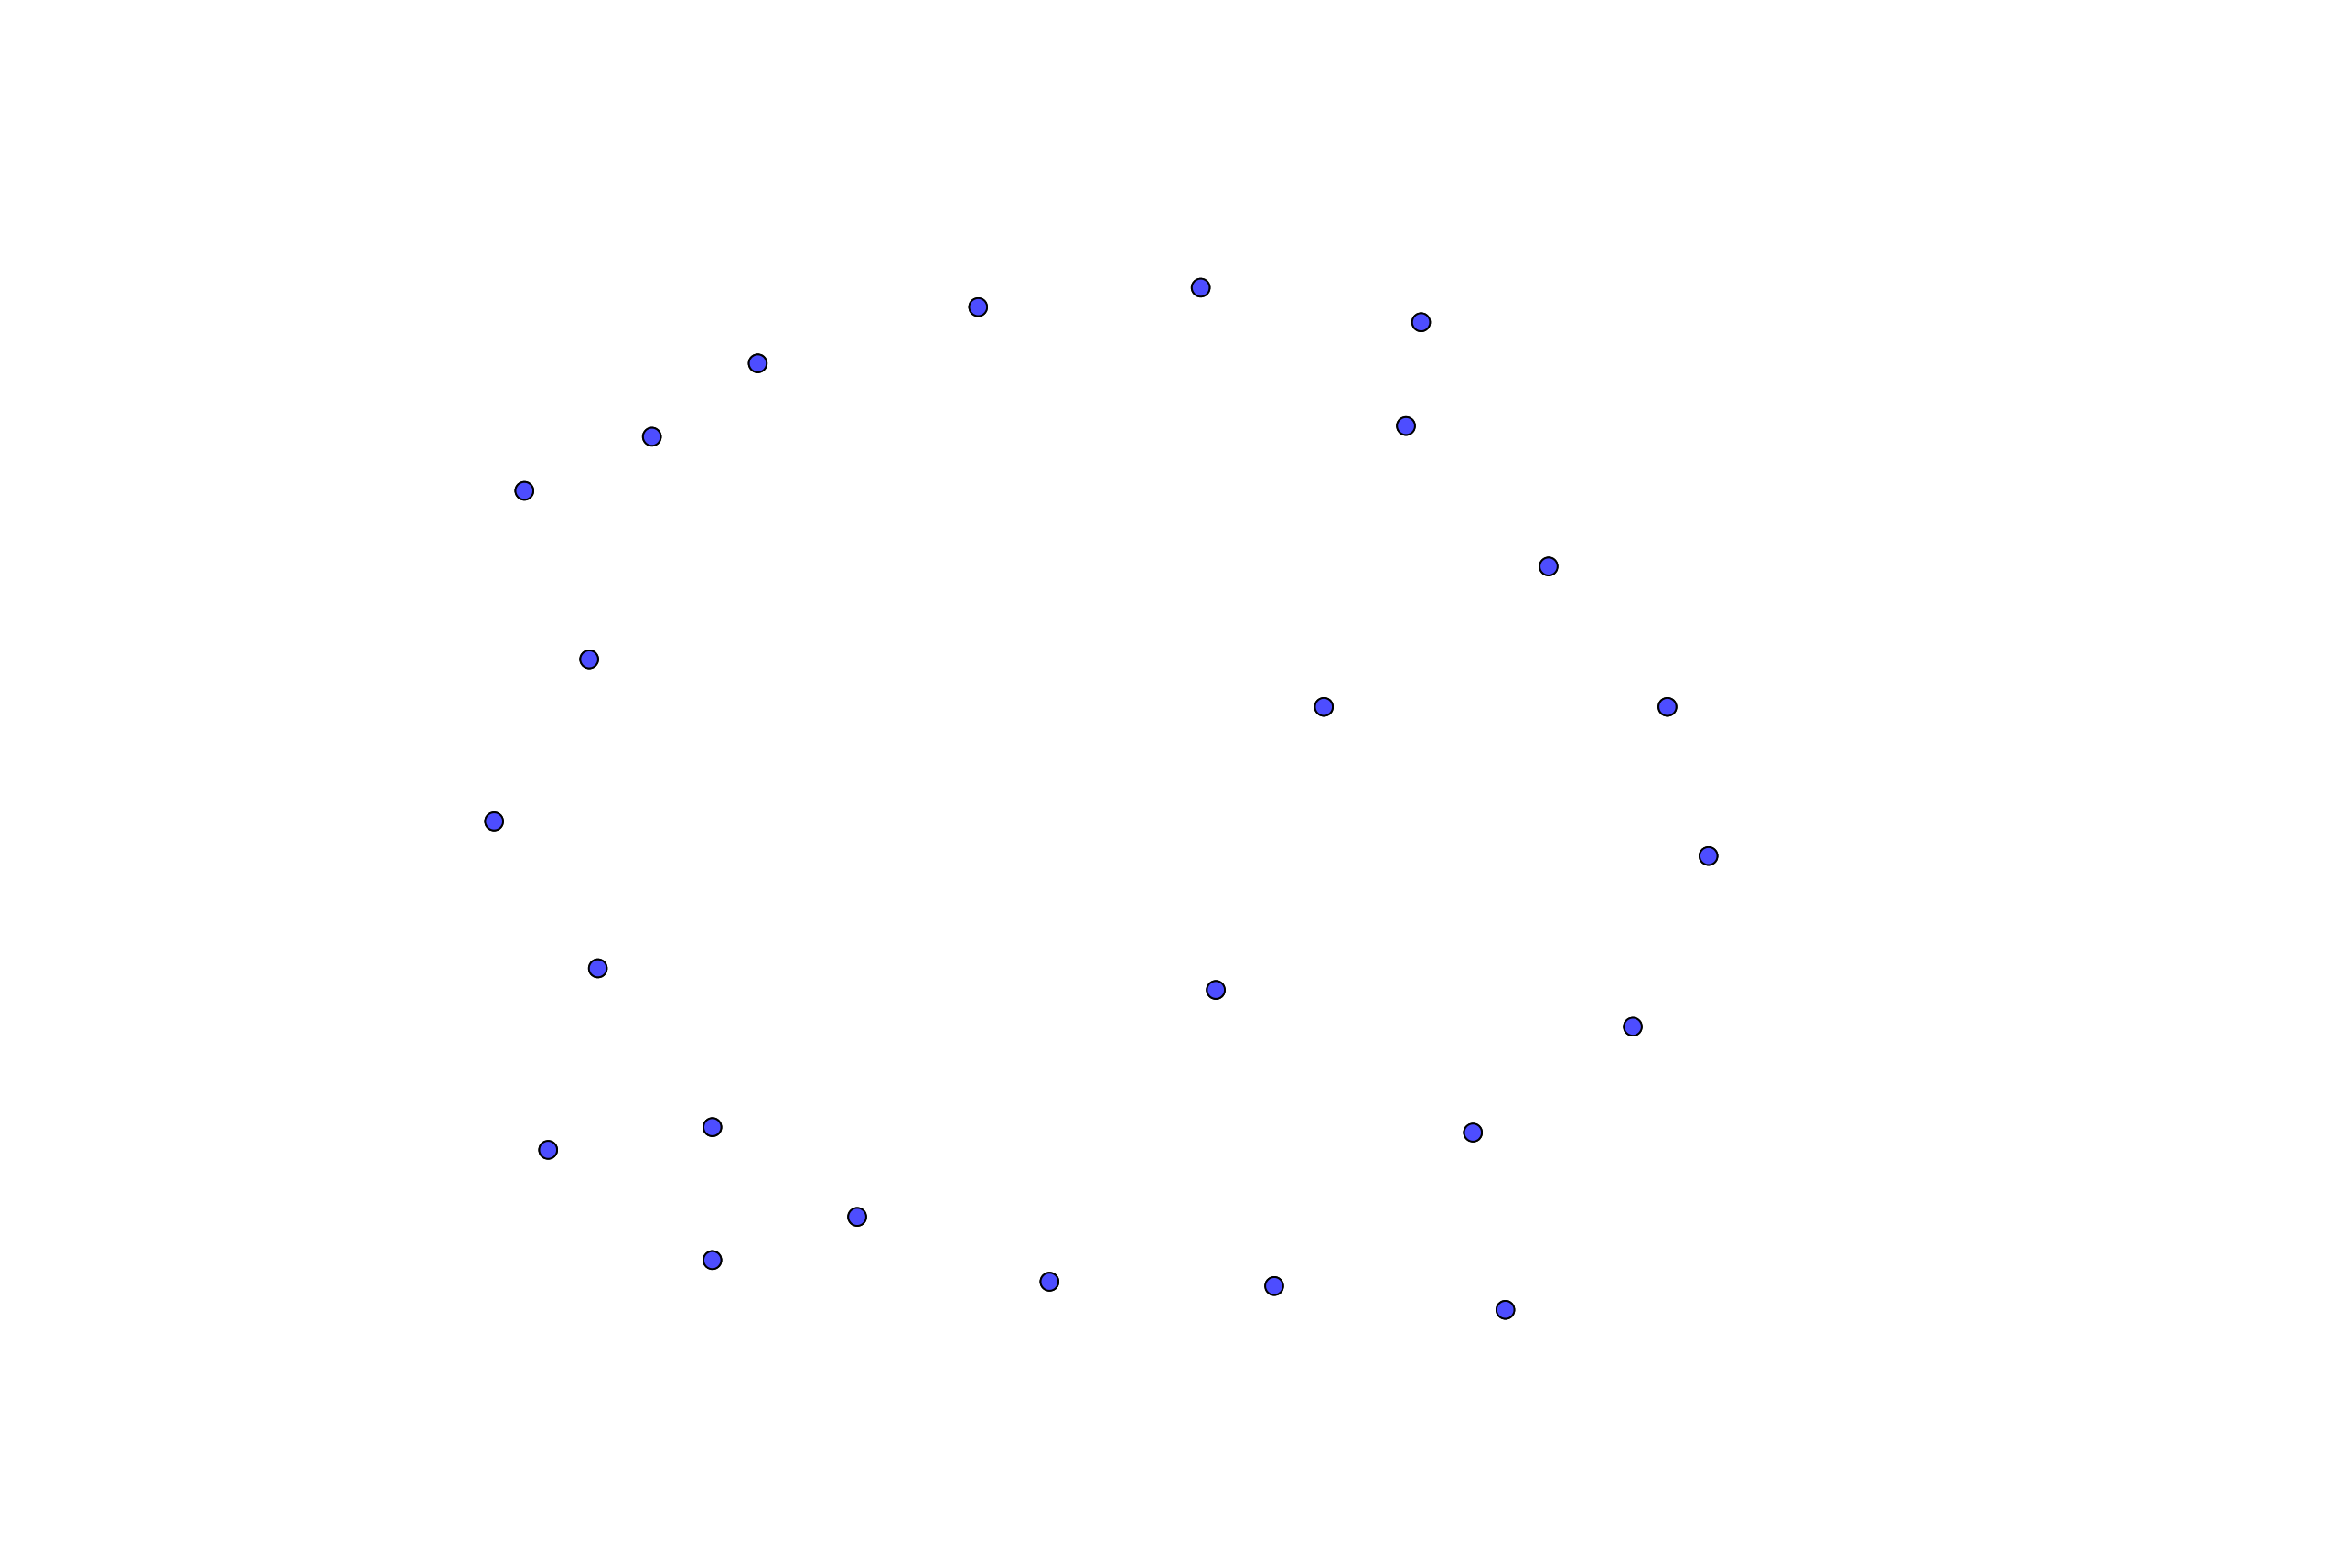
\includegraphics[scale=0.25]{img/cloud002.png}
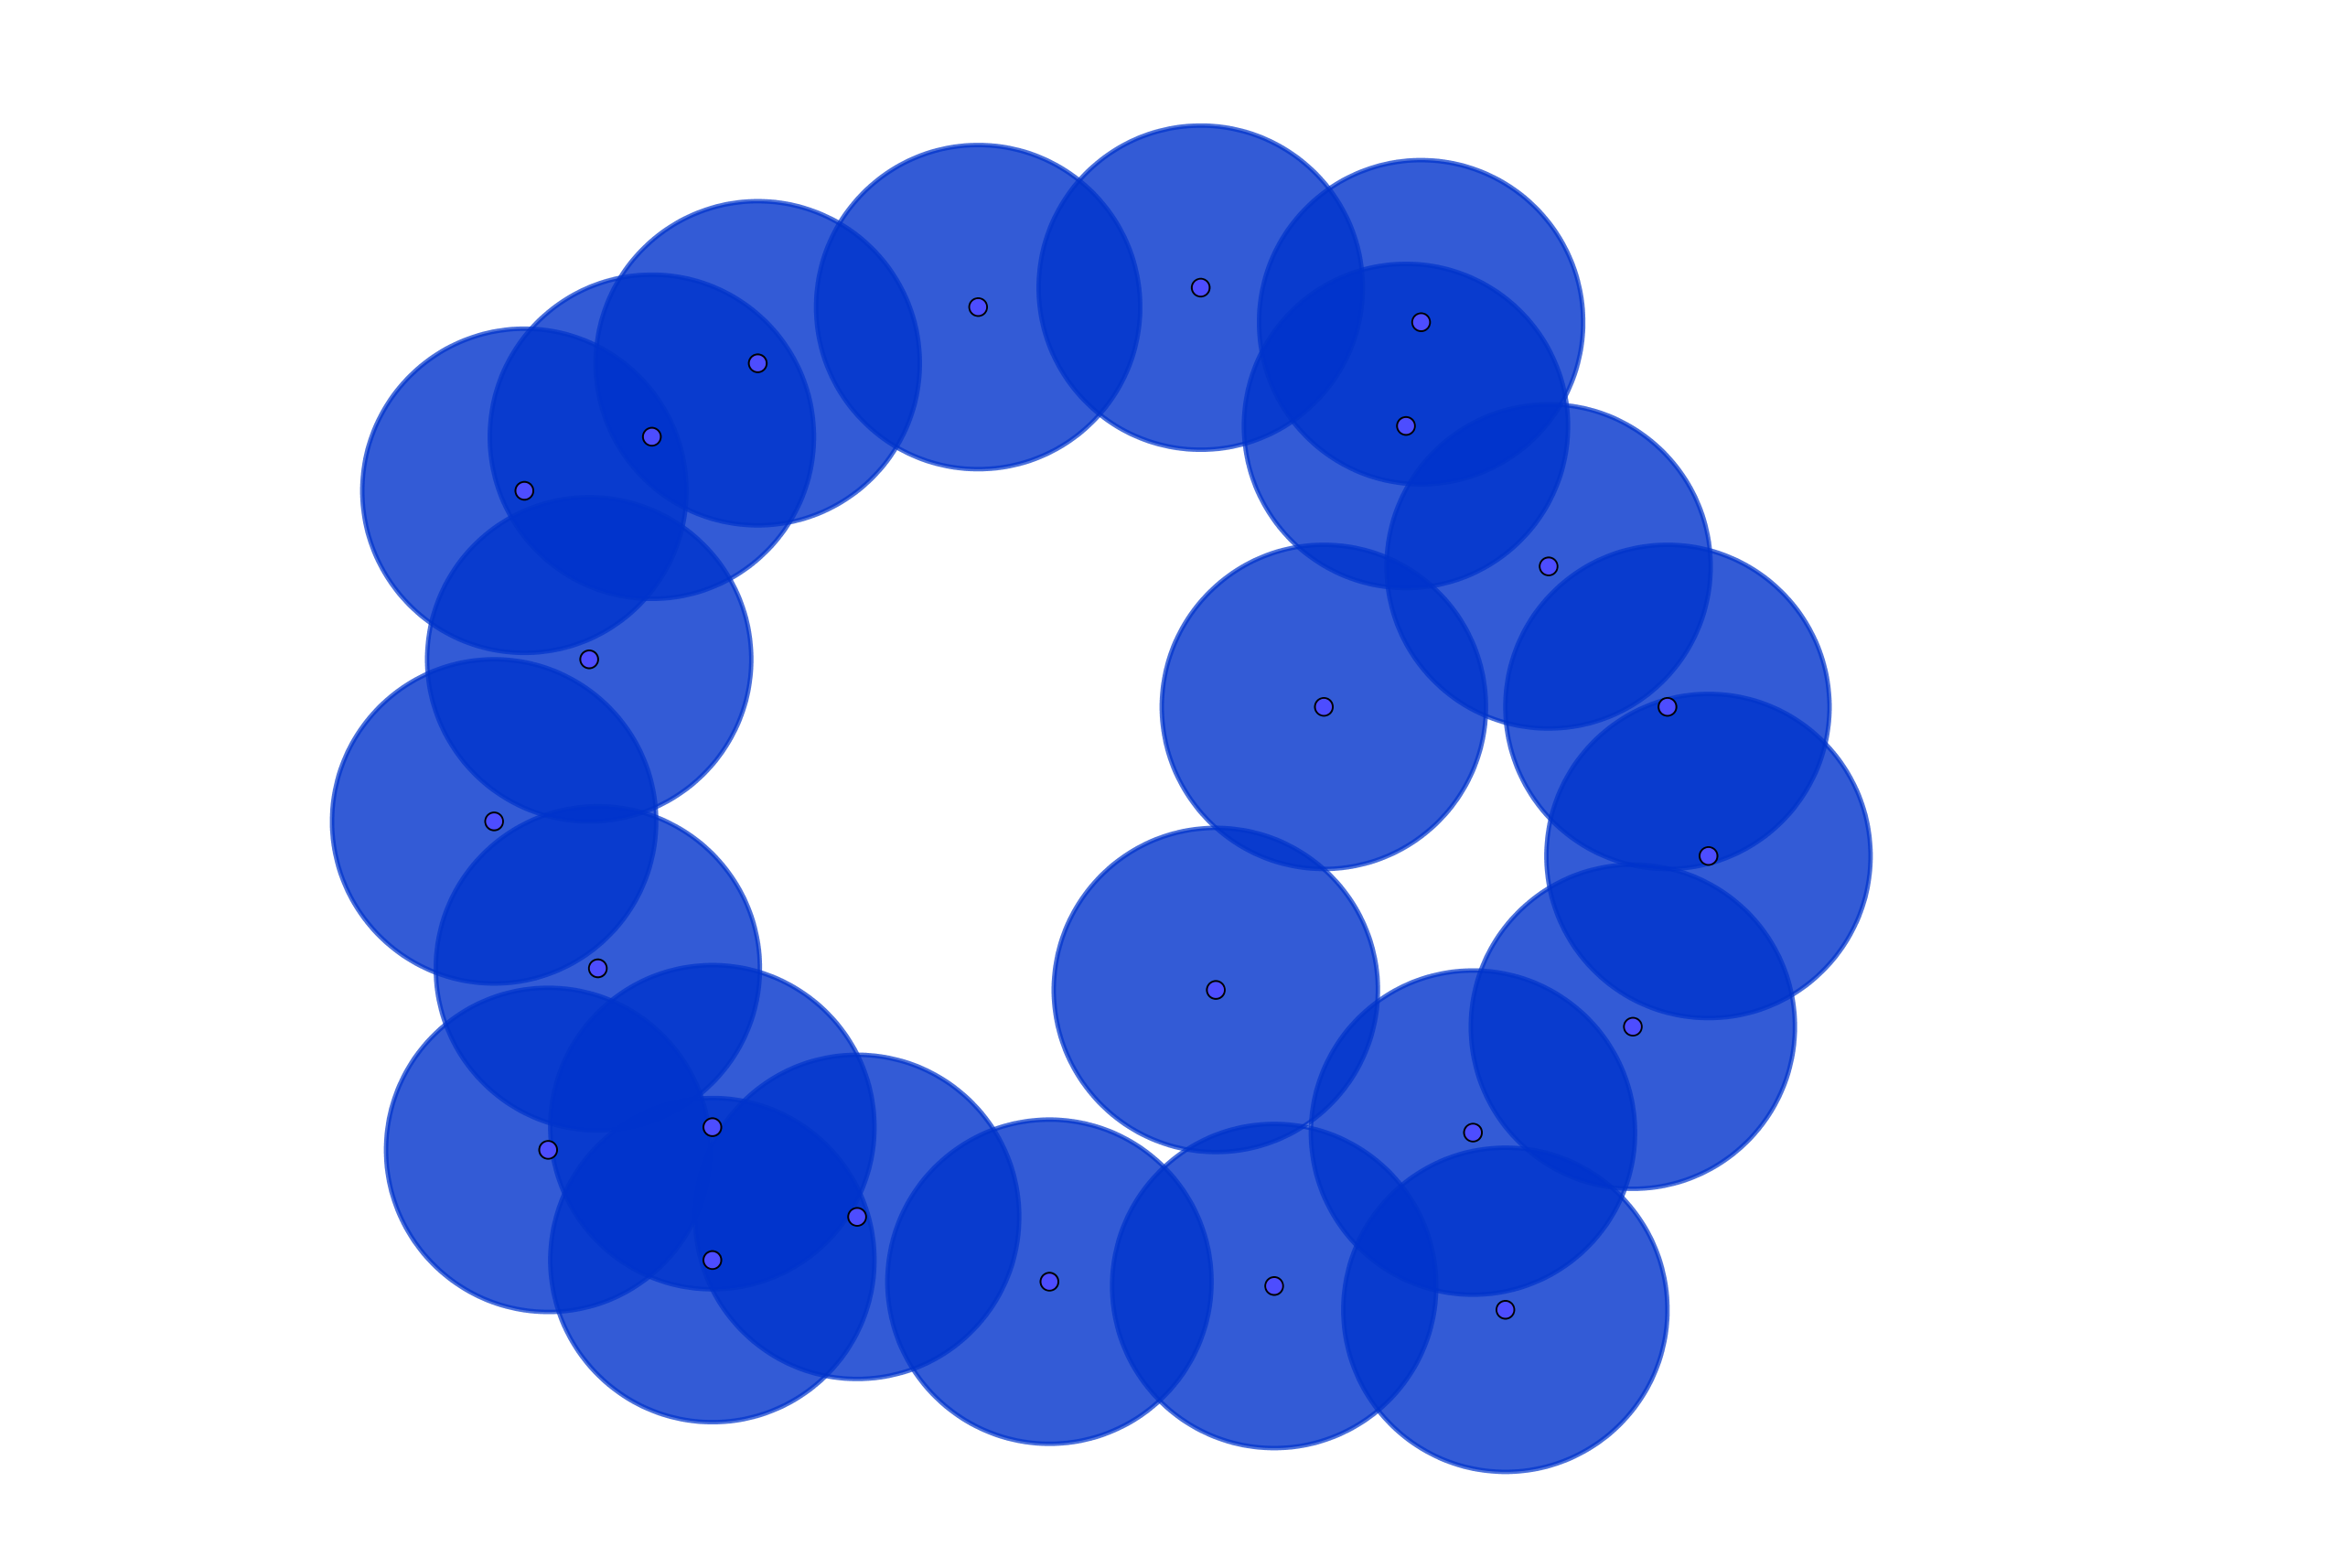
\includegraphics[scale=0.25]{img/cloud152.png} \\
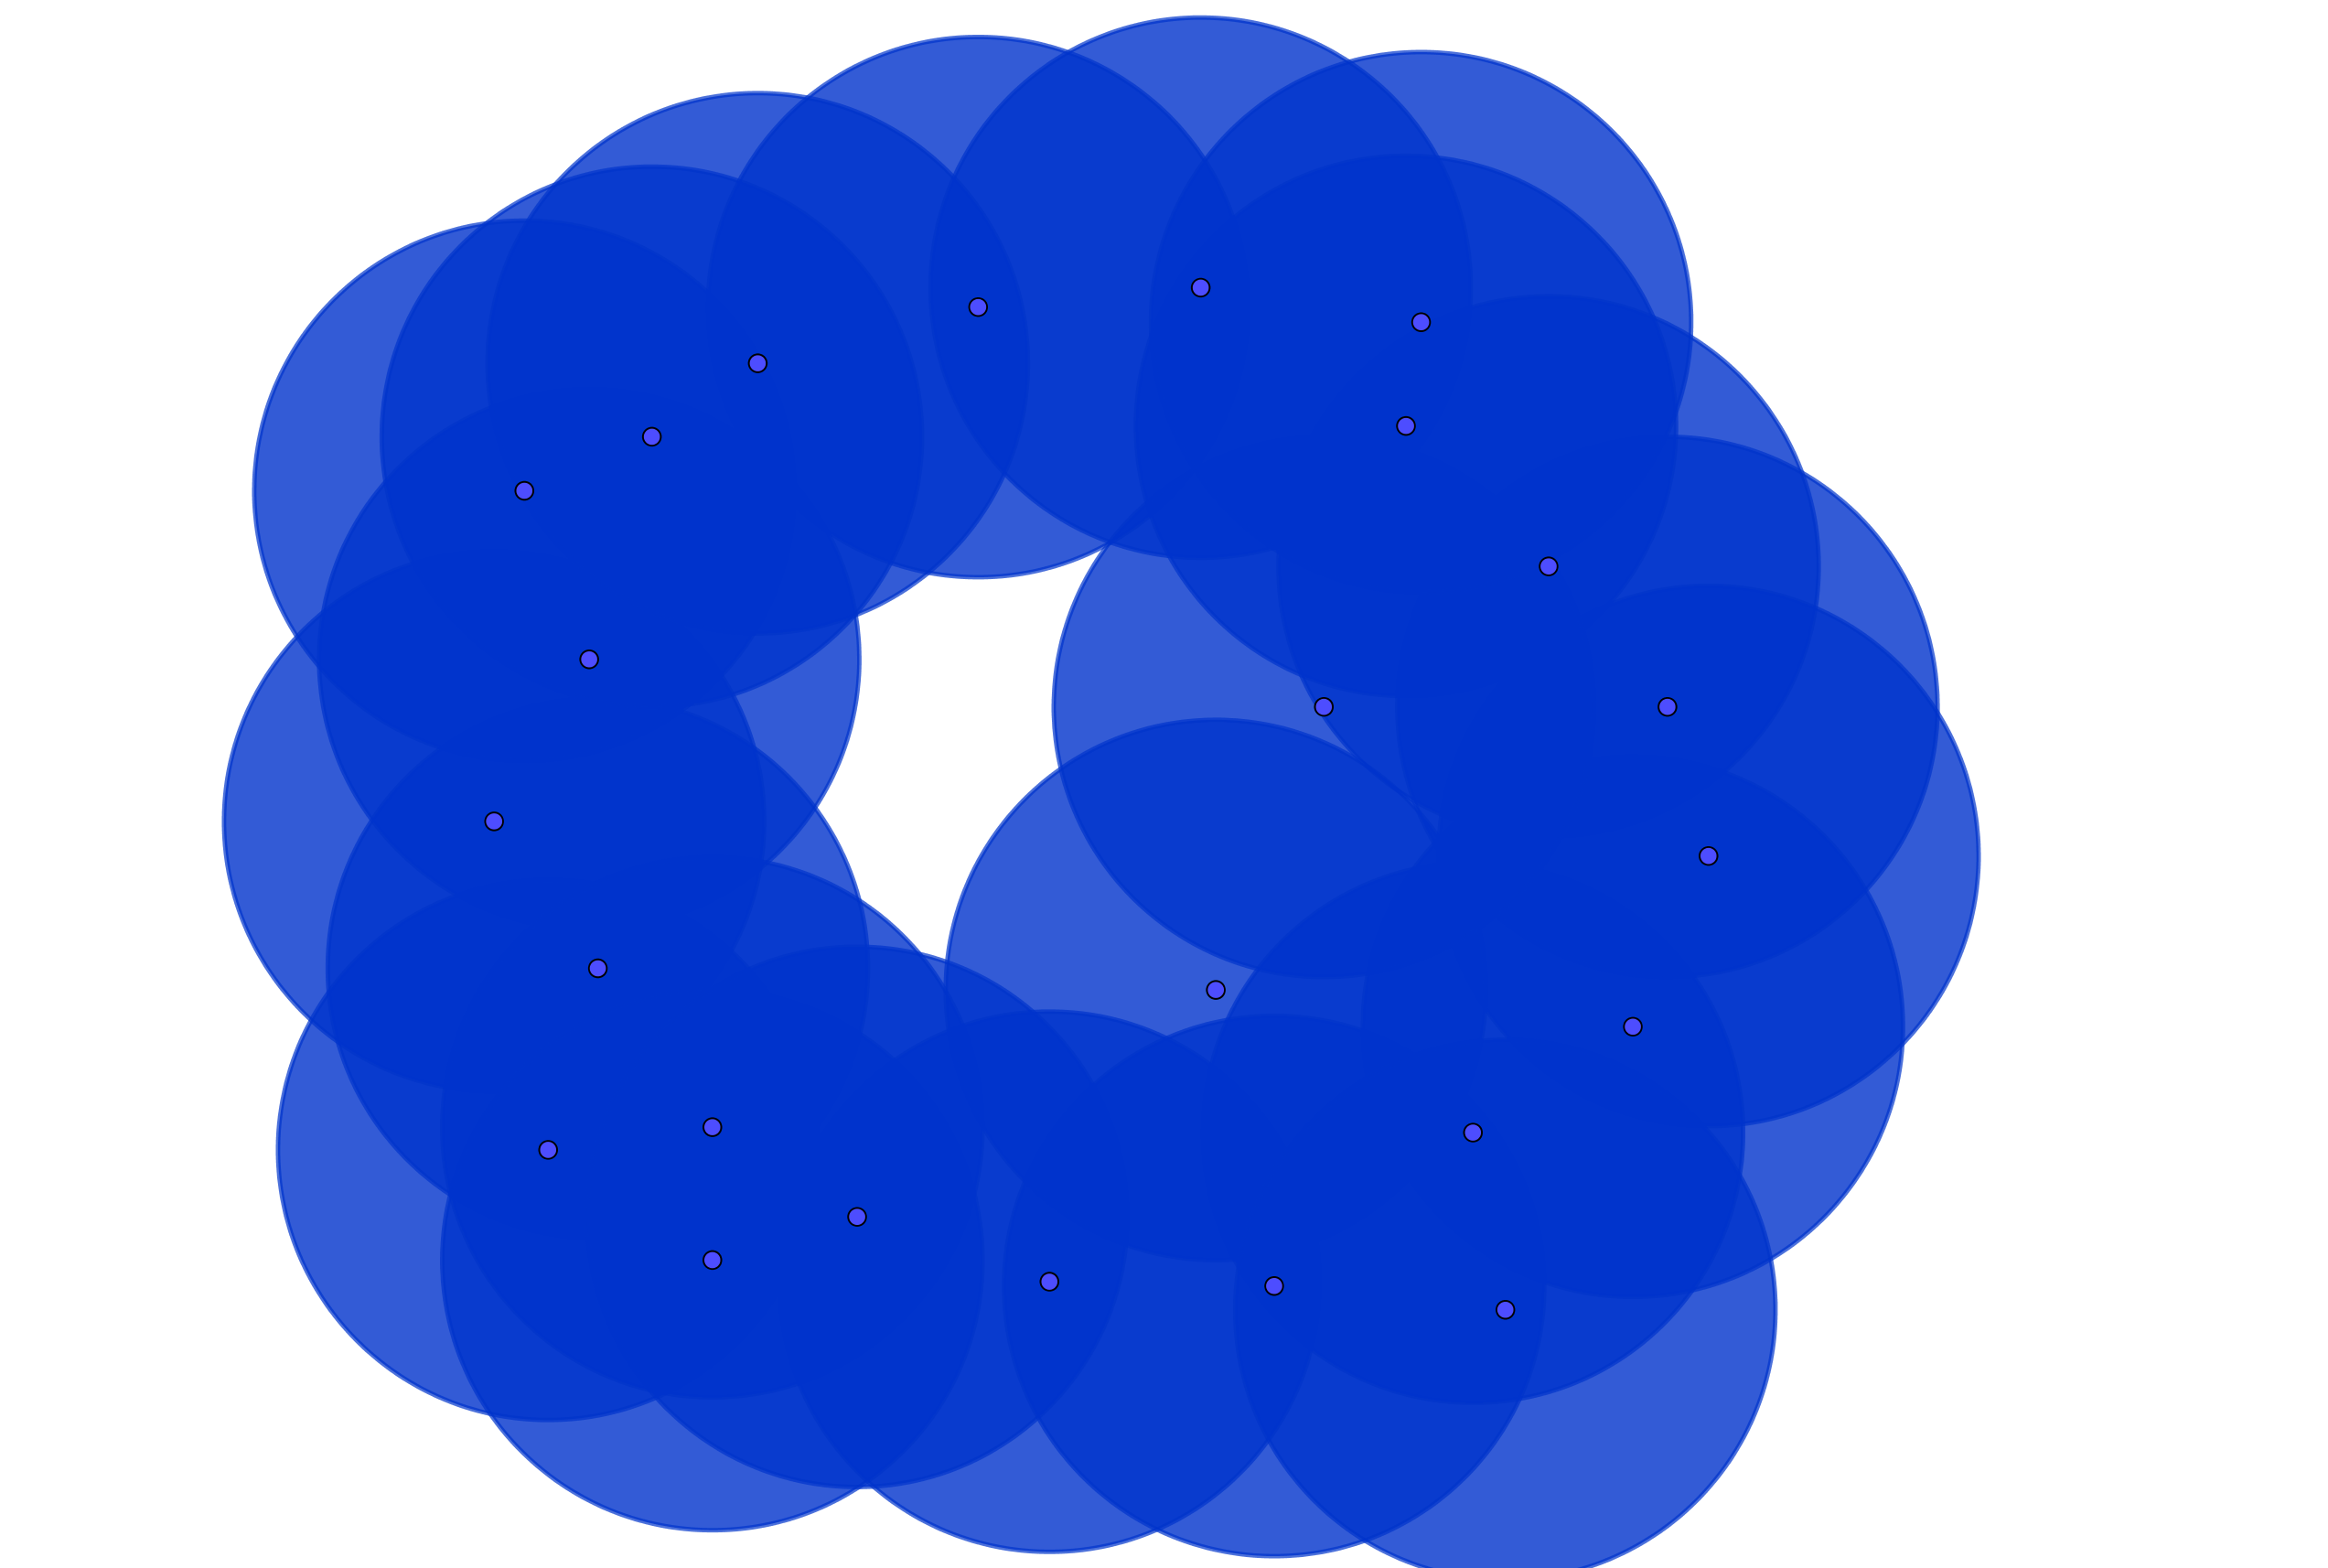
\includegraphics[scale=0.25]{img/cloud252.png}
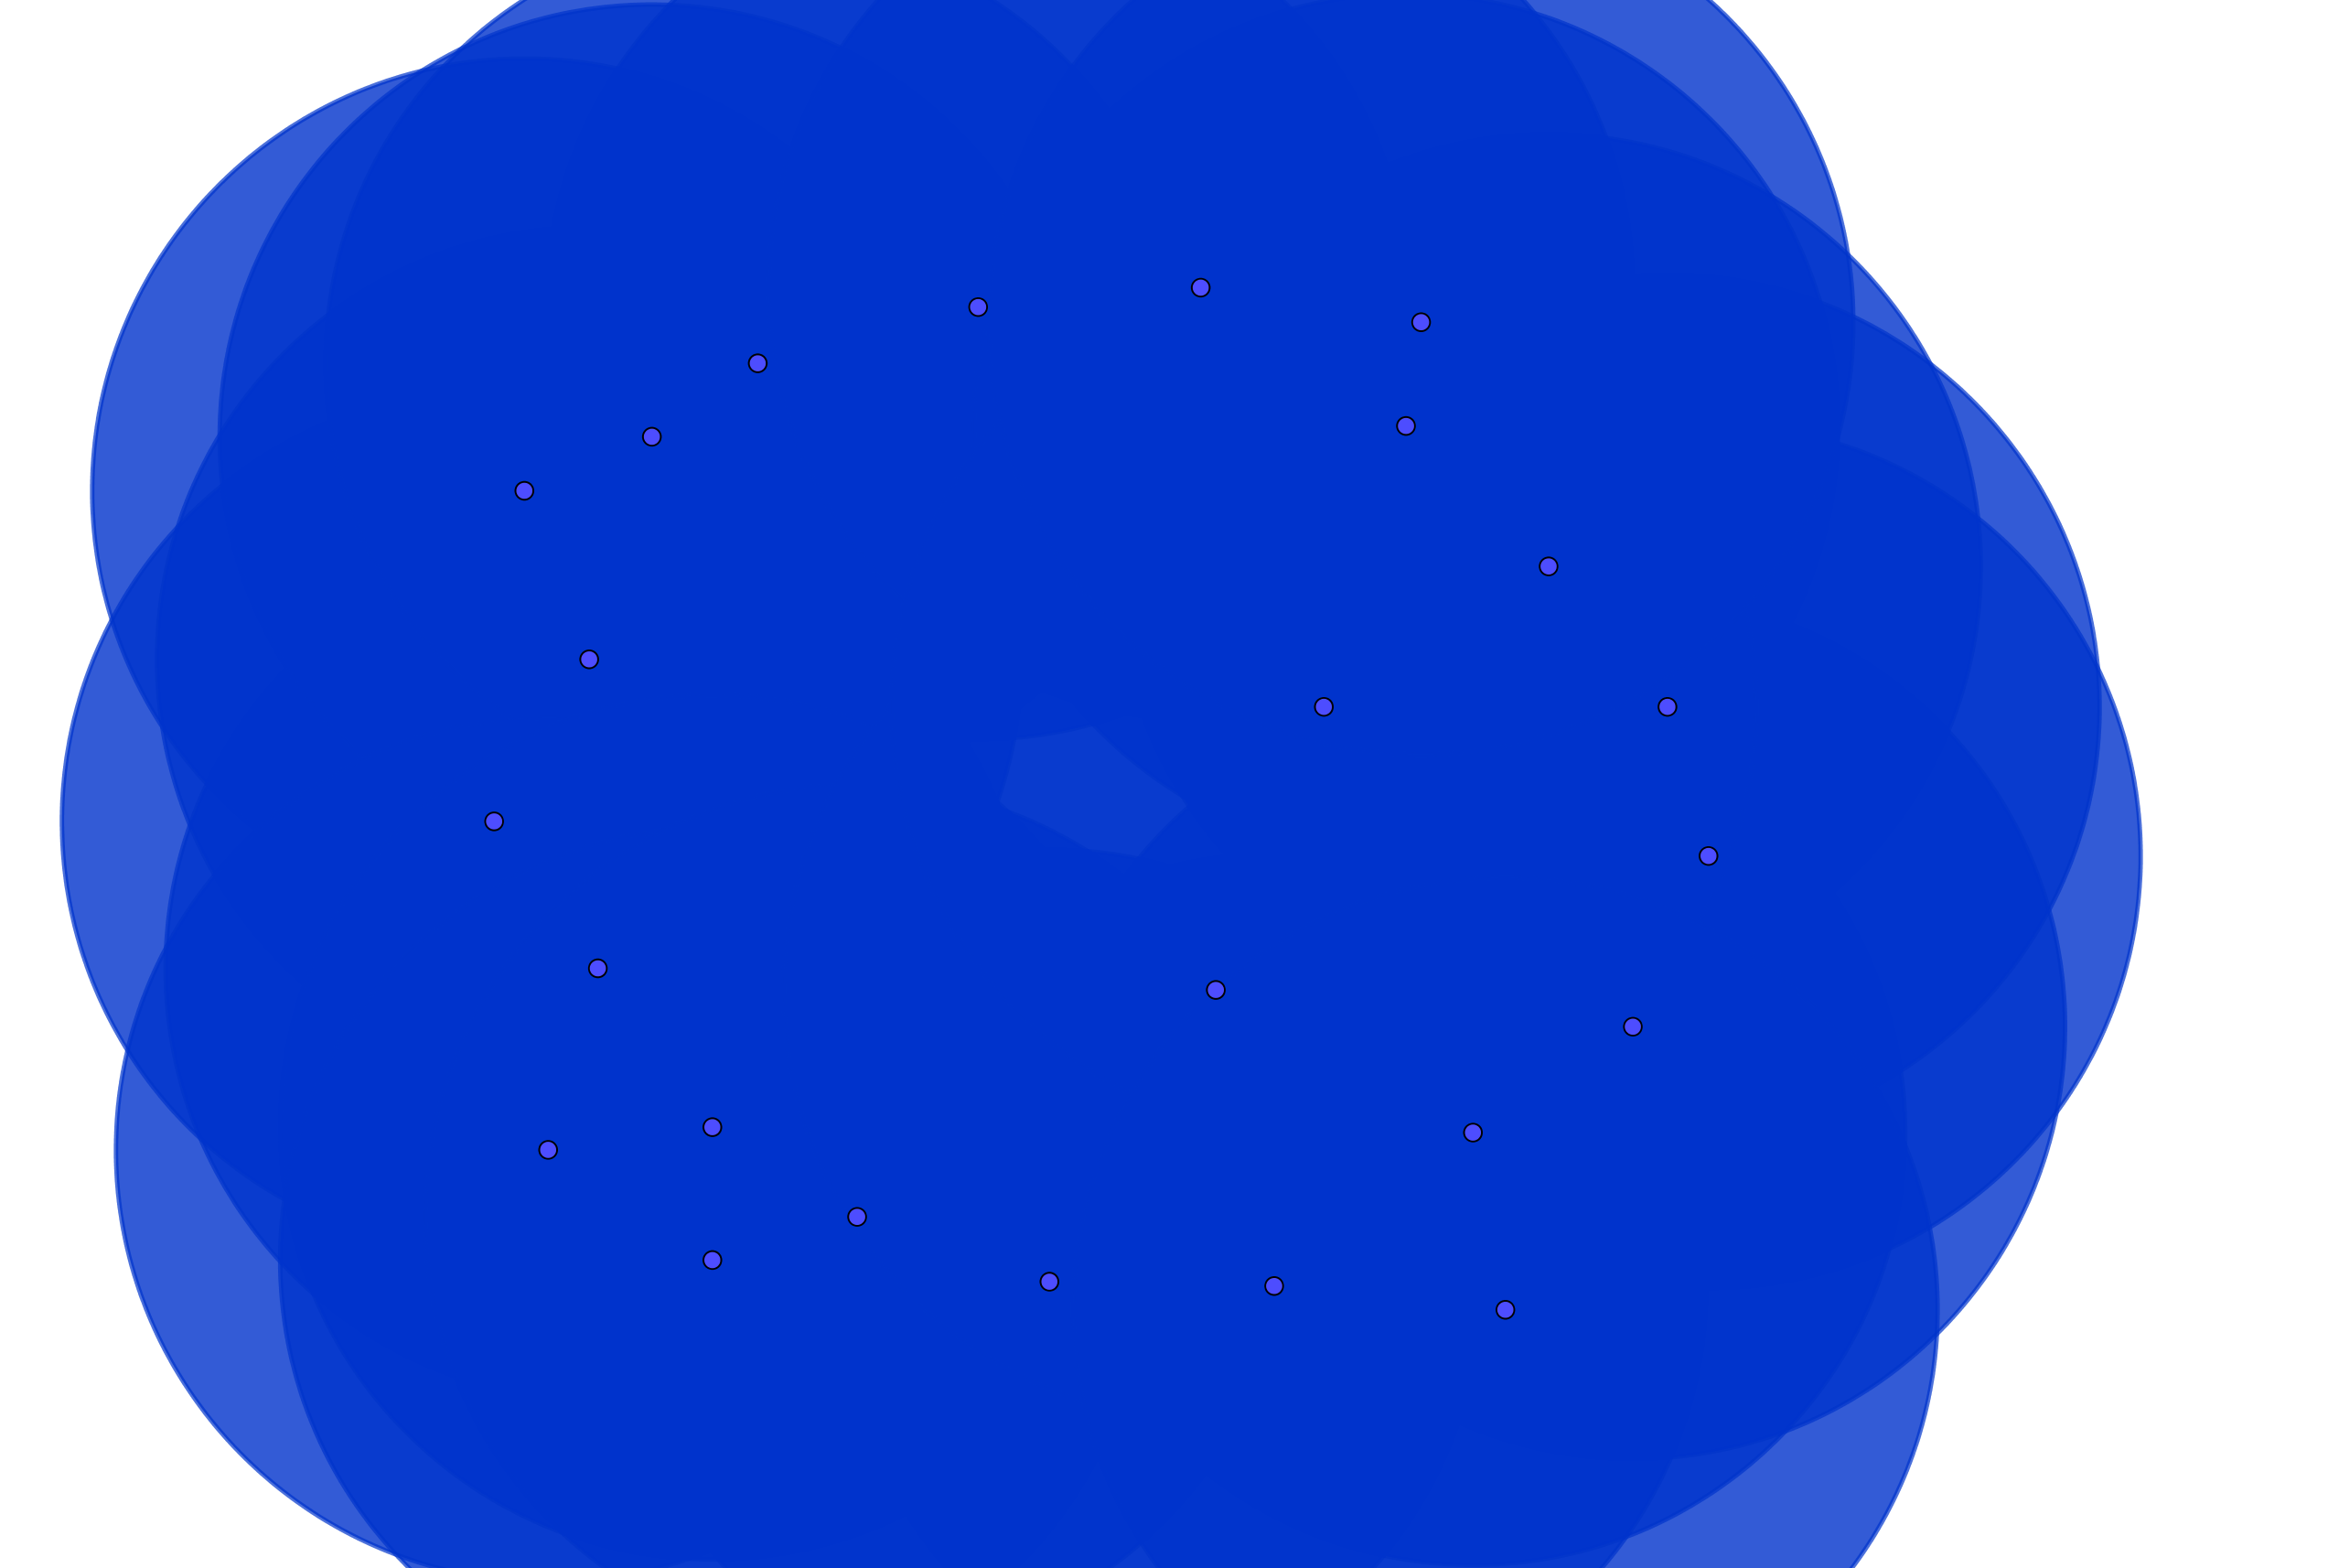
\includegraphics[scale=0.25]{img/cloud402.png}
\caption{Bolas de distinto radio sobre los puntos de una nube de datos}
\label{epsilons}
\end{figure}

Claro que la elección del $r$ más \emph{adecuado} para representar fielmente la nube de datos es todo un tema de debate. Con un $r$ demasiado pequeño se mantienen los grupos de homología del propio $S$, mientras que si $r$ es suficientemente grande se llega al caso de una única componente contráctil. En el ejemplo de la Figura \ref{epsilons} vemos 4 recubrimientos por bolas de una nube de datos con distintos valores de $r$, cada uno de ellos con un tipo de homotopía diferente, y con ello distintos grupos de homología: la primera imagen son $26$ puntos disconexos ($\simeq \sqcup^{26} \{ * \}$), la segunda son dos circunferencias unidas ($\simeq S^1 \vee S^1$), la tercera es una sola circunferencia ($\simeq S^1$) y la última es una sola masa contráctil ($\simeq \{ * \}$).  

Estas construcciones con bolas para distintos $r>0$ forman una familia indexada de espacios que representan la figura que se esconde tras la nube de datos: ésto es, a grandes rasgos, lo que llamamos una \emph{filtración}, que es el elemento base de esta teoría. La homología persistente utiliza filtraciones como ésta para estimar los grupos de homología de la figura subyacente, siendo más factibles aquellos que se dan en un mayor rango de $r$ dentro de la filtración.

El punto clave de las filtraciones que se usan en homología persistente es que cada elemento de la filtración está contenido en el siguiente (como en el caso de las bolas, donde  el espacio creado por un $r' > r$ contiene el espacio creado por $r$) y por ello podemos seguir el rastro de los agujeros que se forman al ir recorriendo la filtración y ver en qué punto se generan y en qué punto mueren. En estas condiciones, el \emph{tiempo de vida} de cada agujero resulta una buena medida de la presencia de dicho ciclo en la figura.

El concepto de homología persistente fue introducido por primera vez por H. Edelsbrunner, D. Letscher y A. Zomorodian en 2002 en su artículo \emph{Topological Persistence and Simplification} \cite{Edelsbrunner} y reformulado pocos años después en 2005 por G. Carlson, A. Collins, L. Guibas y el propio A. Zomorodian en \emph{Persistence barcodes for shapes} \cite{Carlsson}, punto a partir del cual esta teoría comenzó a ganar fuerza. A día de hoy, existe cierta variedad de programas que implementan el método desarrollado por estos autores; destacamos \texttt{PHAT} de U.~Bauer, M.~Kerber y J.~Reininghaus en C++, la librería \texttt{TDA} de B.~Fasy, J.~Kim, F.~Lecci, C.~Maria y V.~Rouvreau para R, y el módulo \texttt{Dionysus} de D.~Morozov para Python.

A lo largo de esta sección, se desarrollarán los conceptos básicos de esta teoría. Comenzaremos hablando de los complejos de Čech y de Vietoris-Rips, que son los dos ejemplos básicos para construir filtraciones. A continuación se definirá formalmente el concepto de filtración y los generadores de persistencia de ésta. Finalmente, hablaremos de diagramas de persistencia y códigos de barras que son los formatos más extendidos para representar los resultados de la homología persistente.

\subsection{Complejos simpliciales}
Las construcciones por bolas de radio $r$ que utilizábamos como ejemplo en el comienzo de ésta sección son una buena forma de entender cómo montar una filtración a partir de la nube de puntos, pero en la práctica no son utilizadas ya que calcular los grupos de homología para un espacio topológico general (mediante homología singular) no es un proceso trivial, ni mucho menos sistemático. En homología persistente el objetivo es encontrar los grupos de homología de una forma algorítmica y para casos generales (de dimensión arbitraria, por ejemplo) donde no se cuenta con la ayuda visual. Es por este motivo que en el cálculo de persistencia se usan habitualmente complejos simpliciales para construir las filtraciones. La homología simplicial nos brinda un método puramente algebraico para calcular los grupos de homología, y con él se puede construir un algoritmo que resuelve el problema en un número determinado (al menos finito) de pasos.

A continuación se definen los dos complejos más ampliamente usados en homología persistente para la construcción de filtraciones.

\subsubsection{Complejos de Čech}
El complejo de Čech es la equivalencia homotópica del recubrimiento mediante bolas en términos de complejo simplicial, y por ello resulta un ejemplo muy didáctico (aunque no tan eficiente en términos computacionales) para comenzar con la homología persistente.

\begin{definicion}
Sea $X$ un espacio topológico y sea $\mathcal{U} = \{ U_i \}_{i\in I}$ una familia de abiertos $U_i \subseteq X$ de éste. Definimos el \emph{nervio} de $\mathcal{U}$ como el conjunto de subconjuntos finitos $\Nrv \mathcal{U} \subseteq \mathcal{P}(I)$ tal que:
\begin{enumerate}
\item $\emptyset \in \Nrv \mathcal{U}$
\item Si $\cap_{j\in J} U_j \neq \emptyset$ para $J\subseteq I$, entonces $J\in \Nrv \mathcal{U}$
\end{enumerate}
\end{definicion}

\begin{definicion}
Sea $S$ un subconjunto finito de un espacio euclídeo $X$, y sea $r > 0$. Definimos el \emph{complejo de Čech} de radio $r$ sobre $S$ como el nervio del recubrimiento $\mathcal{U} = \{ B(x, r)\}_{x \in S}$ y lo denotamos por $C_r(S)$.
\end{definicion}

El recubrimiento definido en el complejo de Čech no es más que el conjunto de bolas de radio $r$ del que hablábamos al comienzo de la sección. El concepto de nervio nos habla, dada una colección de abiertos indexada por un cierto $I$, de los subconjuntos de $I$ cuyos respectivos abiertos intersecan entre ellos. Así pues, el complejo de Čech es una identificación de la bolas ---y por tanto de los puntos---, y de todas las intersecciones entre ellas (véase Figura \ref{cech-vr}). La gracia de simplificar el recubrimiento de bolas a través del nervio es que nos da la posibilidad de tratar en términos de homología simplicial (abstracta).

\begin{proposicion}
Para cualquier colección $\mathcal{U} = \{ U_i \}_{i\in I}$ de abiertos de un espacio topológico $X$, el nervio $\Nrv \mathcal{U}$ es un complejo simplicial abstracto. En particular, todo complejo de Čech es un complejo simplicial abstracto.
\end{proposicion}
\begin{proof}
Sea $\U = \{ U_i \}_{i\in I}$ una colección de abiertos de $X$. Si $\sigma \in \NrvU$ y $\tau \subseteq \sigma$ entonces se tiene $\cap_{i\in\tau} U_i \supseteq \cap_{i\in\sigma} U_i \neq \emptyset$, luego $\tau \in \NrvU$.
\end{proof}

El punto verdaderamente fuerte del complejo de Čech es la equivalencia comentada antes con el recubrimiento de la nube de datos por bolas de radio $r$. Este hecho se debe al siguiente teorema, la demostración del cuál puede consultarse en \cite{Bjorner}.

\begin{teorema}[Teorema del Nervio]
Sea $\U = \{ U_i \}_{i\in I}$ una colección de abiertos de un espacio topológico $X$ compacto tal que para todo $\sigma \in I$ la intersección $\cap_{i\in\sigma}U_i$ es contráctil (si no es vacía), entonces el nervio $\NrvU$ es homotópicamente equivalente a $\U$.
\end{teorema}

\begin{corolario}
Sea $S$ un subconjunto finito de un espacio euclídeo $X$, y sea $r > 0$. El complejo de Čech $C_r(S)$ es homotópicamente equivalente al recubrimiento $\U = \{ B(x,r) \}_{x\in S}$.
\end{corolario}

\begin{proof}
Es inmediata a partir del hecho que el recubrimiento que define el complejo de Čech está formado por bolas abiertas (convexas) y la intersección finita de conjuntos convexos es convexa, y por ende contráctil.
\end{proof}

\subsubsection{Complejos de Vietoris-Rips}
Los complejos de Čech tienen como ventaja esa fuerte relación con el conjunto de bolas sobre la nube de datos, pero su coste computacional es muy elevado, ya que calcular si un conjunto de más de dos bolas se interseca no es trivial. Es por este motivo que los complejos más utilizados en la homología persistente son los complejos de Vietoris-Rips, que son similares al de Čech, pero mirando sólo las distancias entre los puntos de la nube de datos dos a dos. Otro punto a favor del complejo de Vietoris-Rips, a nivel más general y alejado del análisis de datos, es que el complejo de Vietoris-Rips de un conjunto $S$ depende únicamente de la geometría de éste, sin necesidad de considerarlo como subconjunto de un espacio ambiente.

\begin{definicion}
Sea $S$ un conjunto con una métrica definida sobre él y sea $r > 0$. Definimos el \emph{complejo de Vietoris-Rips} de radio $r$ sobre $S$ como
$$  VR_r(S) = \lbrace \sigma \subseteq S \tq \forall x,y \in \sigma, \; d(x,y) < r \rbrace  $$
\end{definicion}

\begin{proposicion}
Todo complejo de Vietoris-Rips es un complejo simplicial abstracto.
\end{proposicion}

\begin{proof}
Sea $VR_r(S)$ el complejo de Vietoris-Rips definido sobre un conjunto $S$ con métrica y $r > 0$. Si $\sigma \in VR_r(S)$ y $\tau \subseteq \sigma$. Dados $x,y \in \tau$ es evidente que $d(x,y)<r$ ya que $x,y \in \sigma$ y $\sigma \in VR_r(S)$. Por tanto, $\tau \in VR_r(S)$.
\end{proof}

Nótese que el complejo Vietoris-Rips $VR_r(S)$ coincide con el complejo de Čech $C_\frac{r}{2}(S)$ en los símplices de dimensión 0 ---que en ambos casos son los puntos de $S$--- y en los de dimensión 1 ---ya que dos bolas $B(x,\frac{r}{2})$ y $B(y,\frac{r}{2})$ intersecan si y sólo si $d(x,y) < r$---. Para dimensiones mayores, sin embargo, encontramos diferencias ya que el conjunto de bolas debe intersecar (todas ellas) para formar un símplex de $C_\frac{r}{2}(S)$, mientras que en $VR_r(S)$ basta que se intersequen dos a dos (véase Figura \ref{cech-vr}). En general, existe una relación directa entre ambos complejos dada en la siguiente proposición.

\begin{proposicion}
Sea $S\subset\R^n$ una un conjunto finito de puntos. Para todo $r>0$ se tienen las siguientes inclusiones
$$ C_{\frac{r}{2}}(S) \subseteq VR_r(S) \subseteq C_r(S) $$
\end{proposicion}

\begin{proof}
Sea $\sigma=\{ x_1,\dots,x_n \} \in C_{\frac{r}{2}}(S)$. Se tiene que $\cap_{i=1}^n B(x_i,\frac{r}{2}) \neq \emptyset$. En particular $B(x_i,\frac{r}{2}) \cap B(x_j,\frac{r}{2}) \neq \emptyset$ ---y por tanto $d(x_i,x_j) < r$--- para todo $x_i,x_j \in \sigma$. De esta forma, $\sigma \in VR_r(S)$.

Sea ahora $\tau=\{ y_1,\dots,y_n \} \in VR_r(S)$. Fijemos un elemento $y_1\in \tau$. Por ser $\tau\in VR_r(S)$, se tiene que $d(y_1,y_i) < r$ ---y por tanto $y_1 \in B(y_i, r)$--- para todo $y_i \in \tau$. Se tiene así que $y_1 \in \cap_{i=0}^n B(y_i,r)$ y por tanto $\cap_{i=0}^n B(y_i,r) \neq \emptyset$. De esta forma, $\tau \in Q_r(S)$.
\end{proof}

\subsubsection{Realización geométrica}

Tanto en el caso del complejo de Čech como en el de Vietoris-Rips hemos remarcado el hecho de que se tratan de complejos simpliciales abstractos. Sus elementos son colecciones de puntos de la nube de datos, no su envolvente convexa. No podemos hablar de símplices \emph{normales} ya que no se tiene independencia afín de los puntos, ni tampoco se puede asegurar que la intersección de dos elementos del complejo sea cara de ambos. Éstas condiciones, sin embargo, no son necesarias para poder definir la homología sobre ellos.

En cualquier caso siempre podemos hablar de la \emph{realización geométrica} de éstos complejos como la unión de la envolvente convexa de cada elemento del complejo, y entender los complejos de Čech y Vietoris-Rips como se muestran en la Figura \ref{cech-vr}. 

\begin{figure}[h!]
\centering
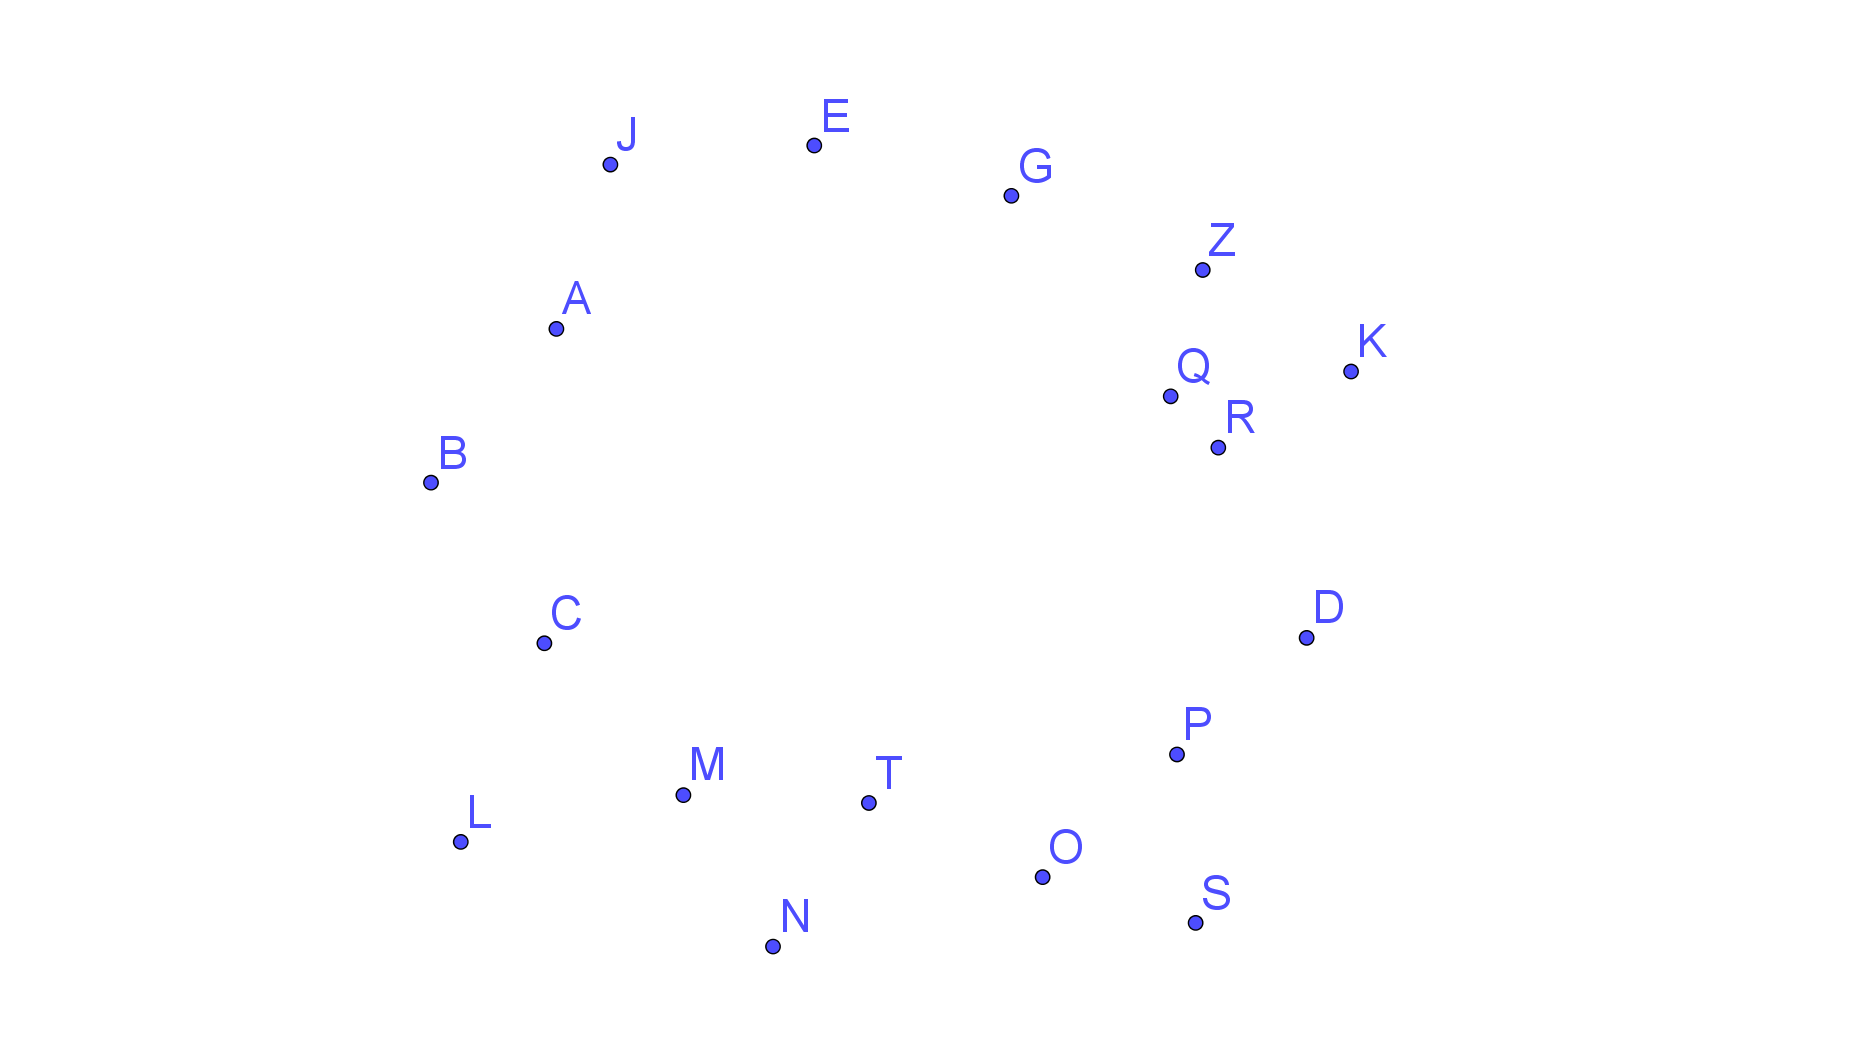
\includegraphics[scale=0.39]{img/puntos.png}
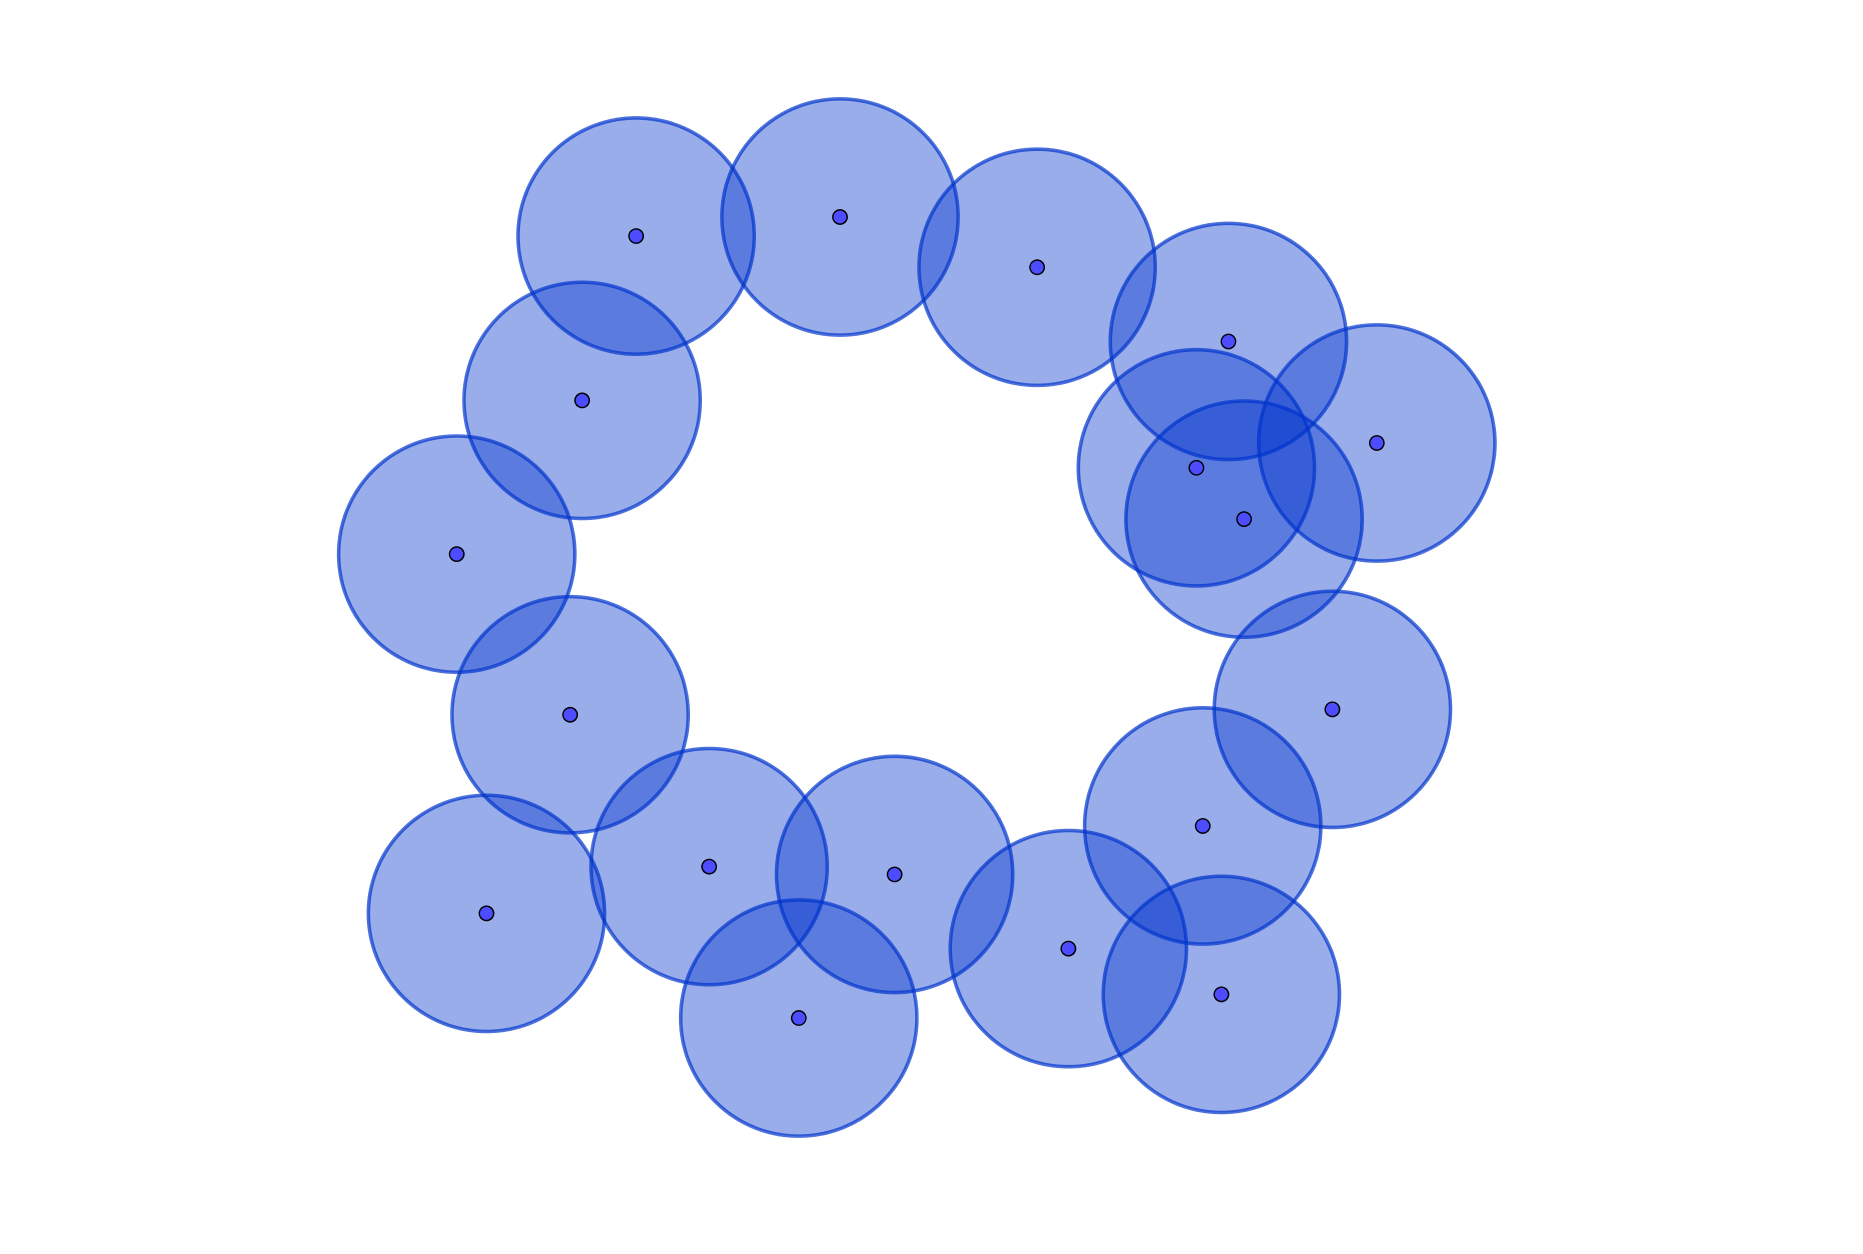
\includegraphics[scale=0.40]{img/cech_bolas2.png}
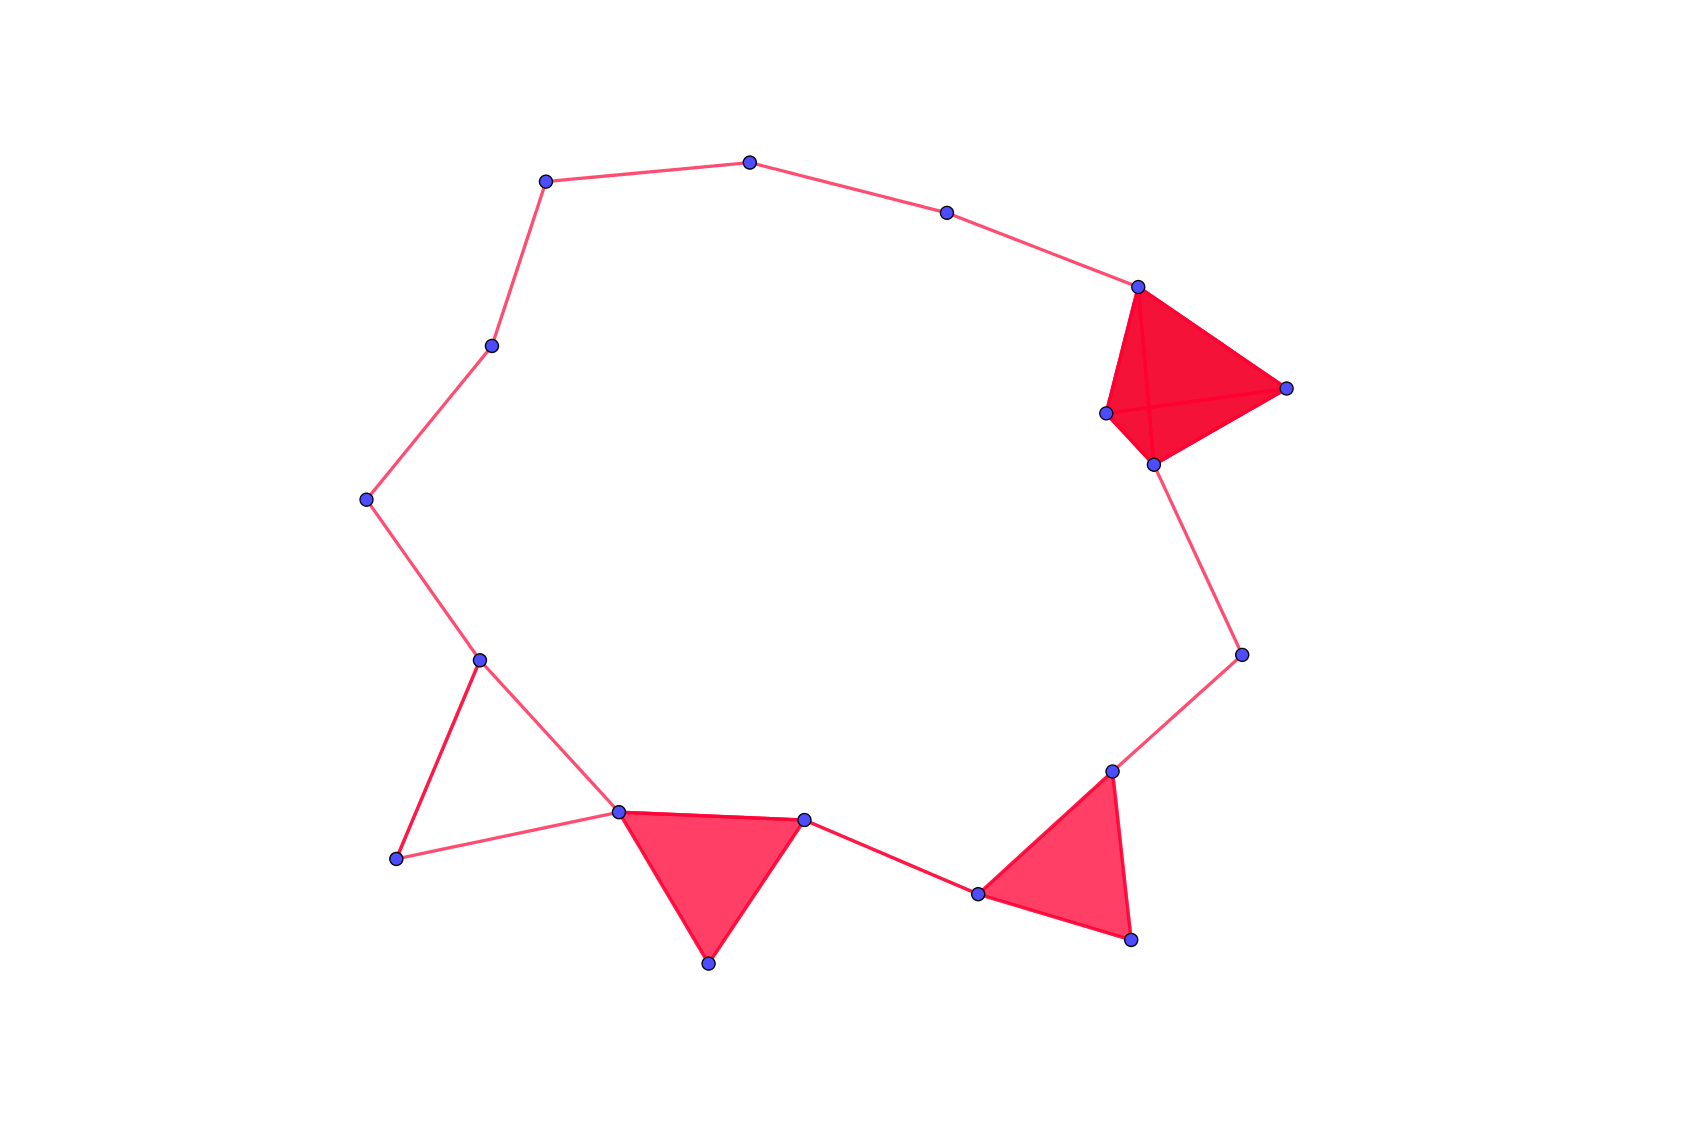
\includegraphics[scale=0.40]{img/cech_complex.png}
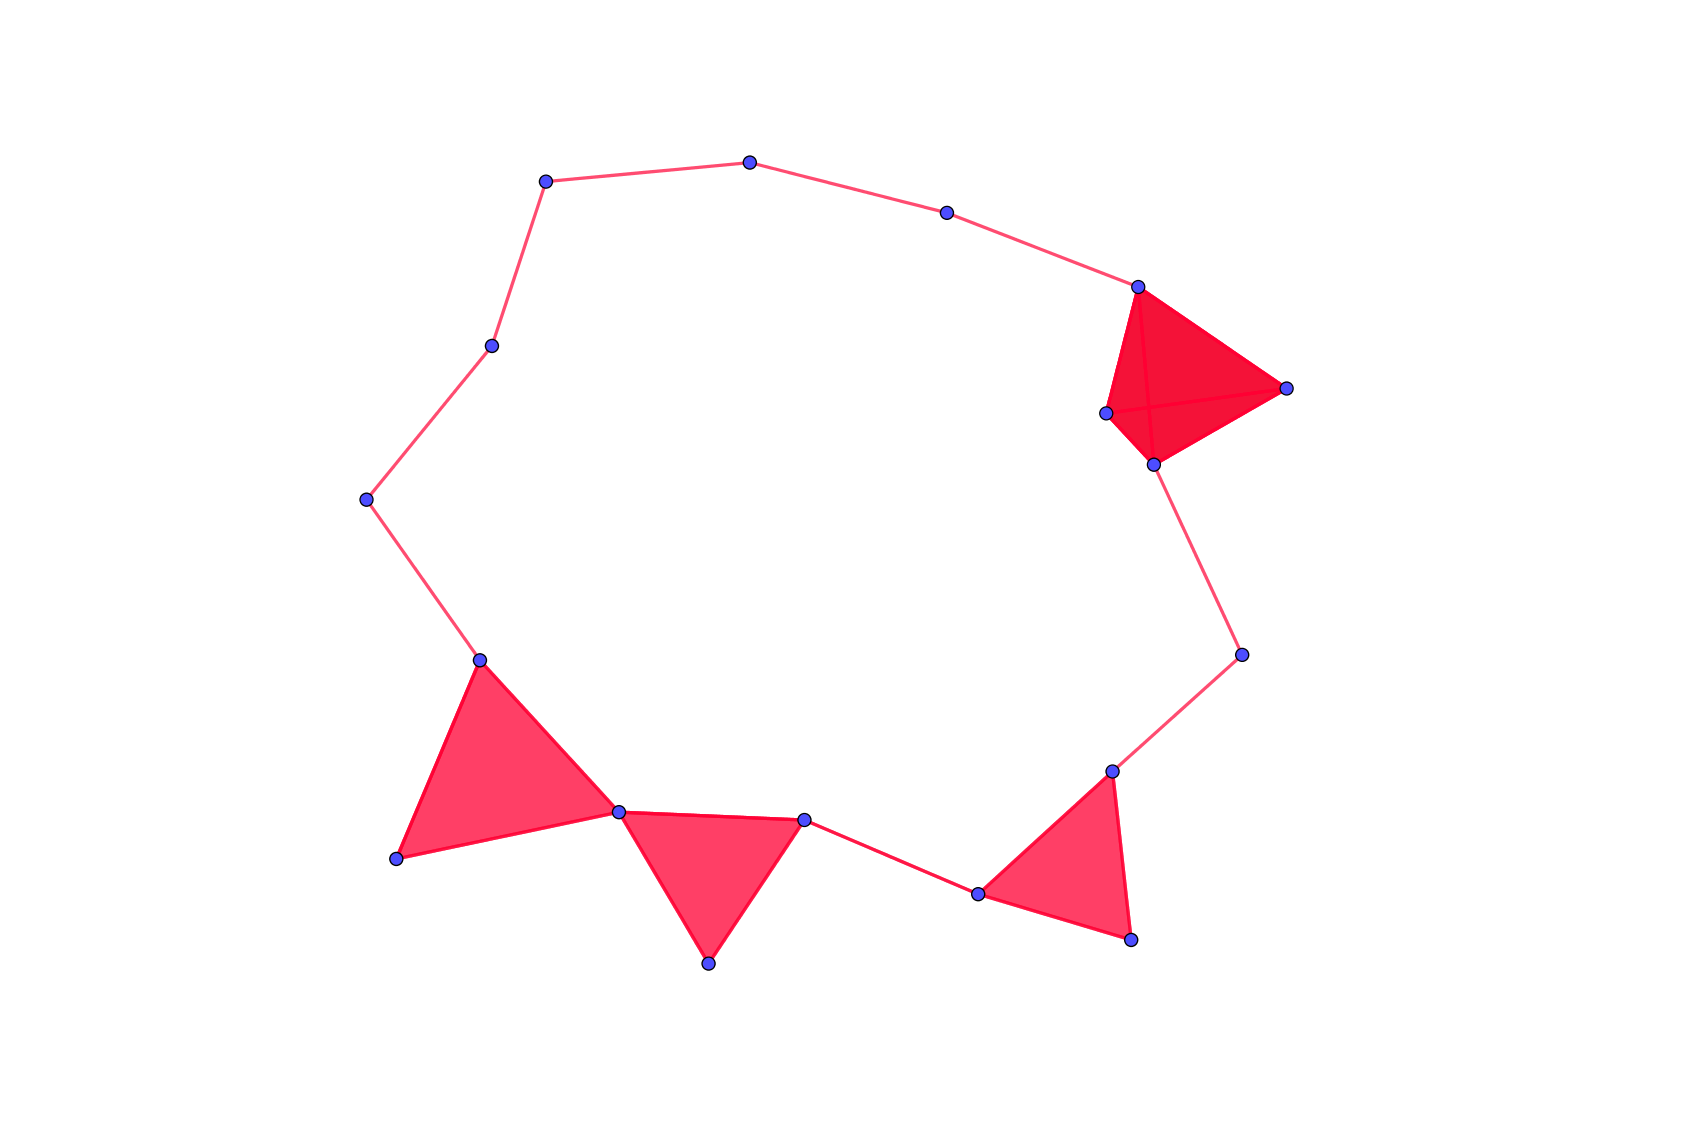
\includegraphics[scale=0.40]{img/vietorisrips.png}
\caption{Construcción a partir de bolas de radio $r$ del complejo de Čech $C_r$ (izquierda) y Vietoris-Rips $VR_{2r}$ (derecha).}
\label{cech-vr}
\end{figure}

Nótese que los puntos $Z$, $Q$, $R$ y $K$ de la Figura \ref{cech-vr} forman un símplex (de dimensión 3) en ambos complejos, pese a ser afínmente dependientes y estar ambientados en $\R^2$. Véase además la ligera diferencia entre ambos complejos: las bolas centradas en $C$, $L$ y $M$ no intersecan las tres, y por ello no forman un símplex en $C_r$, pero sí lo hacen en $VR_{2r}$ ya que intersecan dos a dos.

En ambos casos, la homología simplicial abstracta del complejo de Čech y el de Vietoris-Rips coinciden con la homología singular de su realización geométrica como subespacio de $\R^n$.

\subsection{Filtraciones}

En teoría de conjuntos se define una \emph{filtración} de un conjunto $X$ como cualquier colección ordenada de subconjuntos de $X$ para la cual la inclusión de conjuntos respeta el orden de la colección. Aquí haremos una definición un poco más estricta para tratar filtraciones de complejos simpliciales. 

\begin{definicion}
Dado un complejo simplicial $K$ finito, definimos una \emph{filtración} sobre $K$ como una familia de subcomplejos $\mathcal{F} = \lbrace K_i \subseteq K \rbrace_{i \in I}$ indexados sobre un conjunto ordenado $I$ tal que si $i<j$ entonces $K_i \subseteq K_j$, y además $\emptyset,K \in \mathcal{F}$.
\end{definicion}

Dada una nube de datos $S\in \R^n$, las familias $\mathcal{C} = \{ C_r(S) \tq r \geq 0 \}$ y $\mathcal{VR} = \{ VR_r(S) \tq r \geq 0 \}$ son ejemplos de filtraciones del complejo simplicial de todos los símplex formados por puntos de $S$, i.e., el conjunto $\mathcal{P}(S)$. Éstas son las que llamamos \emph{filtración de Čech} y \emph{filtración de Vietoris-Rips}, respectivamente.

\begin{figure}[h!]
\centering
%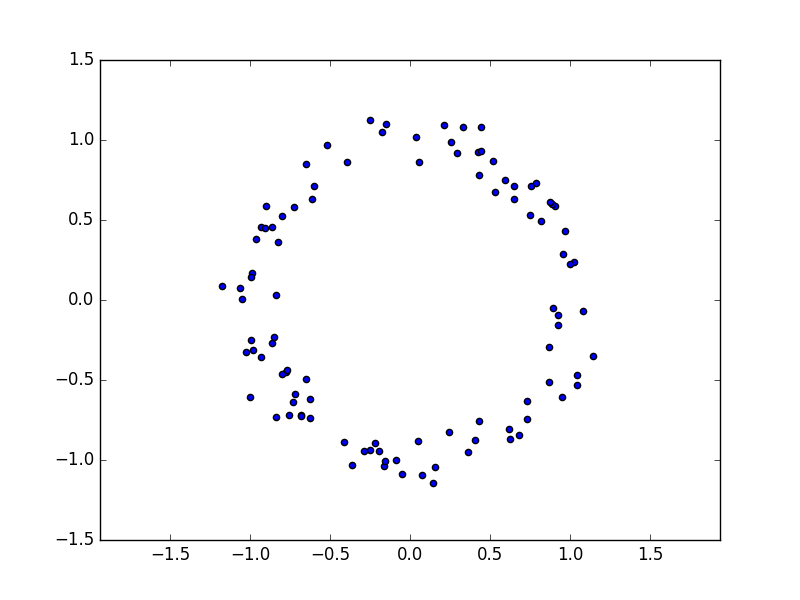
\includegraphics[scale=0.28]{img/figure_1.png}
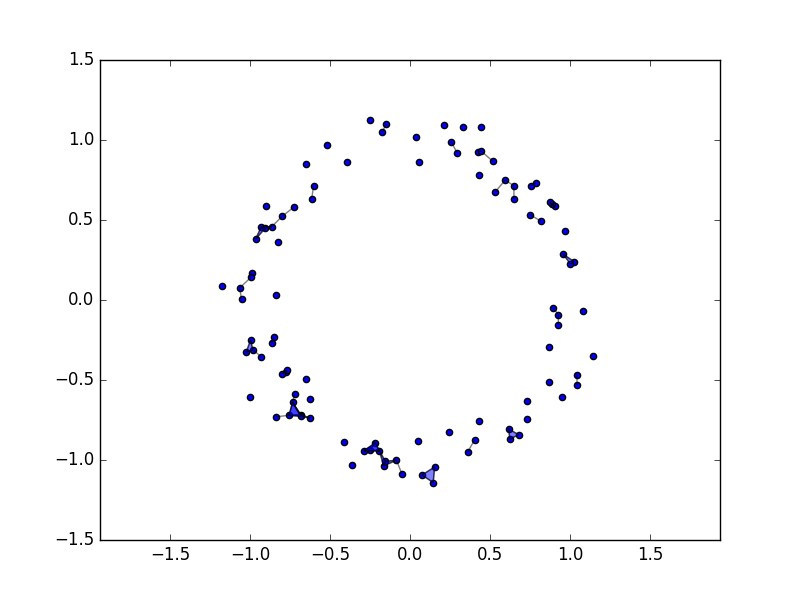
\includegraphics[scale=0.28]{img/figure_2.png}
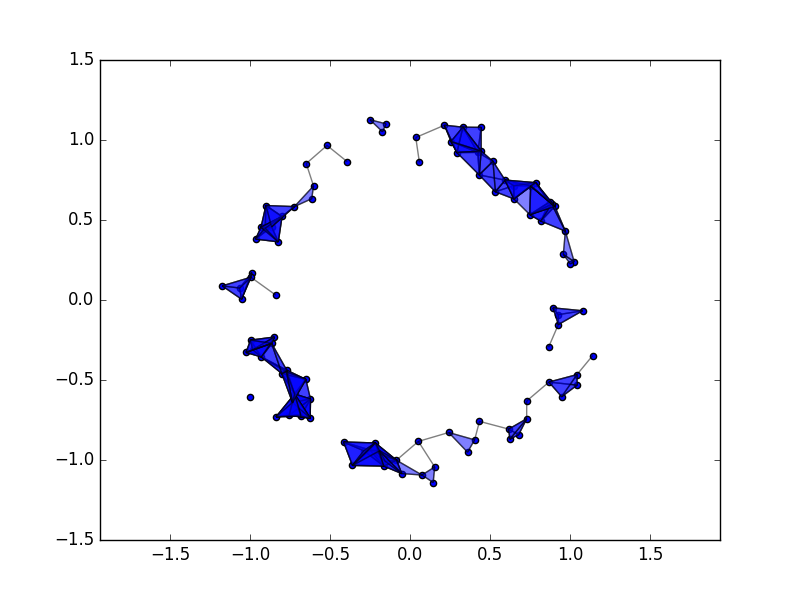
\includegraphics[scale=0.28]{img/figure_3.png}
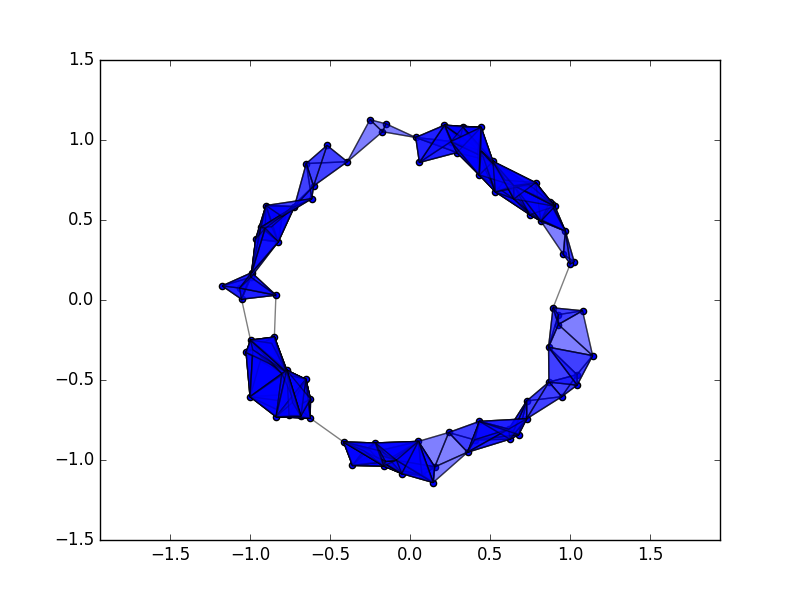
\includegraphics[scale=0.28]{img/figure_4.png}
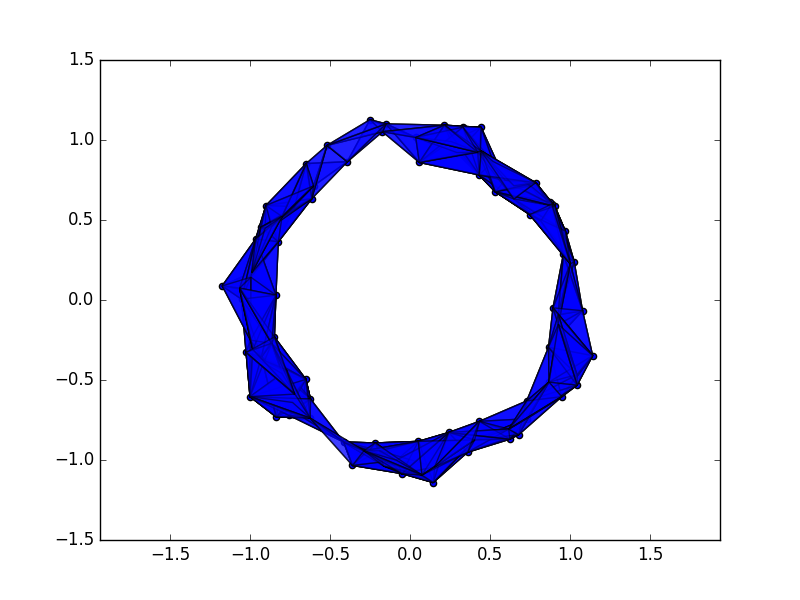
\includegraphics[scale=0.28]{img/figure_5.png}
%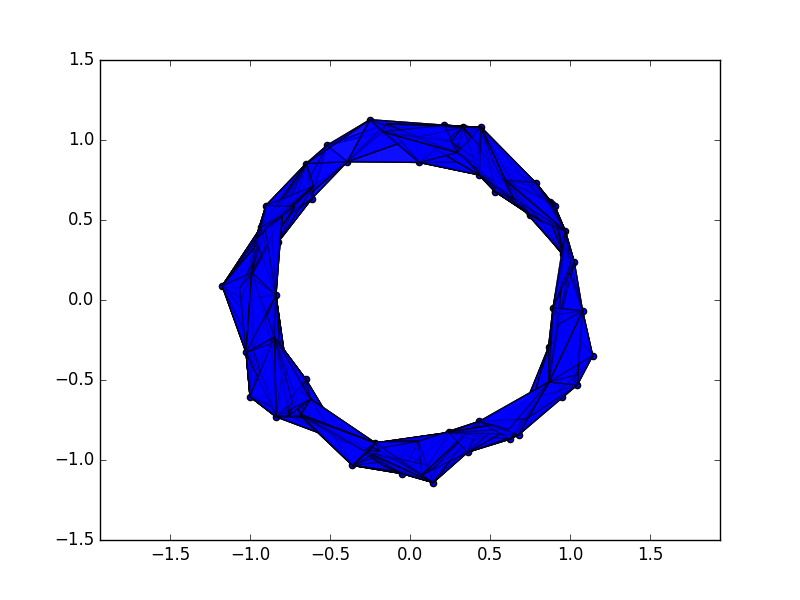
\includegraphics[scale=0.28]{img/figure_6.png}
\caption{Filtración de Vietoris-Rips de una nube de datos.}
\label{filtracion}
\end{figure}

\begin{observacion}
Vale destacar que, pese a que la filtración pueda no ser finita (como es el caso de las filtraciones de Čech y Vietoris-Rips, que se mueven con índices $r \in [0,+\infty)$), sólo habrá un número finito de subcomplejos de $K$ diferentes (si $K$ es un complejo finito, como se supone). Por ello, en toda filtración podemos considerar únicamente los subcomplejos distintos de ésta, asignándole a cada uno su ínfimo índice, y de esa forma escribir la filtración como una cadena finita 
$$ \emptyset = K_{i_0} \subset K_{i_1} \subset \dots \subset K_{i_n} = K $$
con $i_0,\dots,i_n \in I$.
\end{observacion}


\subsubsection{Filtraciones subnivel}
Una forma de construir filtraciones es a partir de una función definida sobre el complejo $K$. Si $\map{f}{K}{\R}$ es una aplicación sobre $K$ que es no decreciente para secuencias crecientes de caras, i.e., $f(\sigma)\leq f(\tau)$ si $\sigma$ es una cara de $\tau$, entonces para todo $a \in \R$ la antiimagen $K_a=f^{-1}((-\infty,a])$ es un subcomplejo de $K$ y se tiene una filtración $\mathcal{F}=\{K_a\}_{a \in \R}$. 

En general, esta forma de construir filtraciones puede extenderse a toda aplicación $\map{f}{K}{I}$ definida en un conjunto ordenado $I$ y, de hecho, resulta una definición equivalente para filtración. Un ejemplo sencillo es el caso de Vietoris-Rips; si $S\in\R^n$ es una nube de datos y $K=\mathcal{P}(S)$, la filtración de Vietoris-Rips es la filtración que se induce de la aplicación $\map{f}{K}{\R}$ definida por $f(\sigma) = \max \{d(x,y) \tq x,y\in \sigma \}$.

\subsection{Persistencia}
Supóngase que se tiene una filtración $\mathcal{F}$ sobre un complejo $K$ de la forma $ \emptyset = K_{i_0} \subset K_{i_1} \subset \dots \subset K_{i_n} = K $. La inclusión de complejos $K_{i_j} \subset K_{i_k}$ para $i_j<i_k$ induce un homomorfismo $\map{f_p^{i_j,i_k}}{H_p(K_{i_j})}{H_p(K_{i_k})}$ en los grupos de homología de los complejos $K_{i_j}$ y $K_{i_k}$. En general, para todo $p\geq 0$ se tiene una cadena de homomorfismos
$$  H_p(K_{i_0}) \stackrel{f_p^{i_0,i_1}}{\rightarrow} H_p(K_{i_1}) \stackrel{f_p^{i_1,i_2}}{\rightarrow} \cdots \stackrel{f_p^{i_{n-1},i_n}}{\rightarrow} H_p(K_{i_n}) $$
donde además los extremos son triviales para $p>0$ si $K$ es contráctil.

Esta cadena de morfismos nos da una relación de equivalencia entre los generadores del $p$-ésimo grupo de homología de dos elementos de la filtración $K_i$ y $K_j$. Decimos que un generador $g_1 \in H_p(K_i)$ equivale a un $g_2 \in H_p(K_j)$ si $f_p^{i,j}(g_1) = g_2$. Con ello se define una relación de equivalencia en el conjunto de generadores de toda la filtración\footnote{La reciprocidad debe forzarse. Se impone que si $g_1 \sim g_2$ entonces $g_2 \sim g_1$.}. Este concepto de ver como \emph{persisten} los generadores de los grupos de homología en la filtración es el punto crucial de la homología persistente.

\begin{definicion}
Sea $K$ un complejo simplicial y $\{K_i\}_{i\in I}$ una filtración sobre éste. Sea $g\in H_p(K_i)$ un generador del $p$-ésimo grupo de homología del elemento $K_i$ de la filtración.
\begin{enumerate}
\item Definimos el \emph{nacimiento} de $g$ como $\tau_B (g) = \inf \{ t\in I \tq g \in \Img{f_p^{t,i}} \}$.
\item Definimos la \emph{muerte} de $g$ como $\tau_D (g) = \inf \{ t\in I \tq f_p^{i,t} (g) = 0 \}$. En caso de que $\{ t\in I \tq f_p^{i,t} (g) = 0 \} = \emptyset $ diremos que $\tau_D = \infty$.
\end{enumerate}
\end{definicion}

Nótese que éstas definiciones respetan la equivalencia $\sim$ que hemos definido, i.e., dos generadores de distintos puntos de la filtración que son equivalentes tienen el mismo punto de nacimiento y de muerte, y por ello podemos extender la definición al conjunto de generadores bajo esta relación.

\begin{notacion}
Si $\mathcal{F}=\{K_i\}_{i \in I}$ es una filtración sobre un complejo simplicial $K$, denotaremos $G(\mathcal{F})$ al conjunto de \emph{generadores persistentes de la filtración}, que son los generadores de cada elemento de la filtración cociente la relación de equivalencia $\sim$ . Sobre los elementos $g \in G(\mathcal{F})$ se extiende la definición de instante de nacimiento $\tau_B(g)$ y de muerte $\tau_D(g)$.
\end{notacion}

\subsection{Métodos de representación de los resultados}

A continuación introducimos brevemente los \emph{diagramas de persistencia} y los \emph{códigos de barras} que son las dos formas más habituales de presentar el resultado de la homología persistente sobre una filtración.

\subsubsection{Diagramas de persistencia}
Los diagramas de persistencia fueron introducidos por H. Edelsbrunner, D. Letscher y A. Zomorodian en \cite{Edelsbrunner} en el nacimiento de la homología persistente y sigue siendo a día de hoy la herramienta más habitual para representar los resultado de ésta.

Supóngase que se tiene una nube de datos sobre la cual se construye una filtración $\mathcal{F}$ indexada sobre $\R^+$ y se han calculado los instantes de nacimiento y muerte de todo elemento $g \in G(\mathcal{F})$.

Un diagrama de persistencia es una gráfica 2D donde se representan los puntos $(\tau_B(g), \tau_D(g))$ para todo $g \in G(\mathcal{F})$. Habitualmente, se representan por separado los puntos correspondientes a distintos tipos de generadores (distintas dimensiones, o distinta torsión), o bien se utilizan distintos colores para distinguirlos dentro de una misma gráfica.

Como es obvio, todos los puntos estarán por encima de la bisectriz del primer cuadrante ya que $\tau_D(g) > \tau_B(g)$. La distancia vertical de estos puntos a la bisectriz indica la \emph{vida} de este generador ---podemos decir que cuanto más separado se encuentre un punto de la bisectriz, más peso tiene el grupo generado por éste en el correspondiente grupo de homología de la figura subyacente de la nube de datos---. Muchos autores unen cada punto a la bisectriz para apreciar de forma más clara cuáles tienen una vida más larga.

\begin{figure}[h!]
\centering
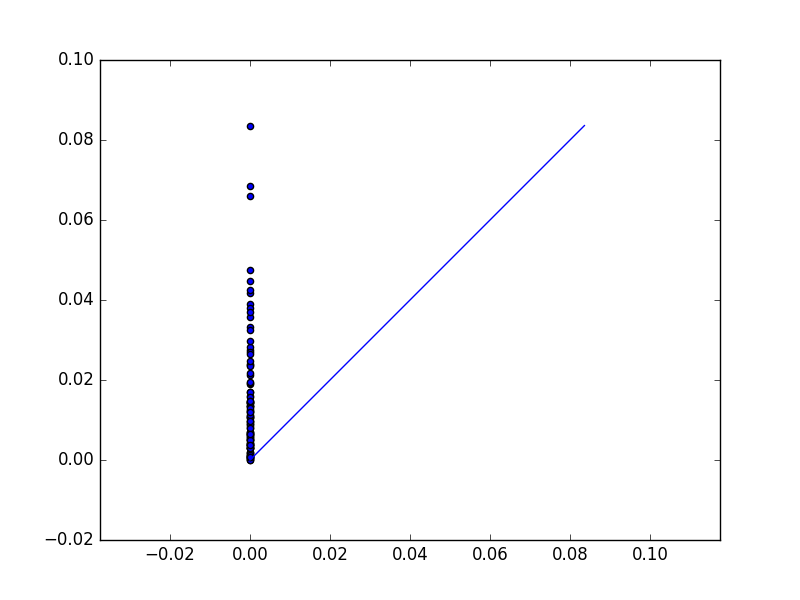
\includegraphics[scale=0.33]{img/persistence0.png}
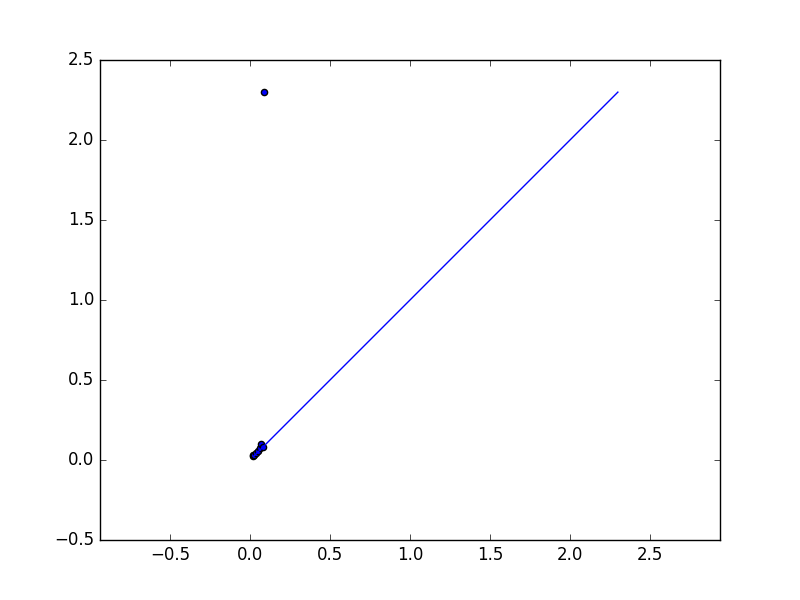
\includegraphics[scale=0.33]{img/persistencediagram.png}
\caption{Diagramas de persistencia de la filtración de la Figura \ref{filtracion}.}
\label{diagramas}
\end{figure}

En la Figura \ref{diagramas} se puede ver un ejemplo de diagramas de persistencia, hechos con el módulo \texttt{Dionysus} de Python. Éstos corresponden a la filtración de Vietoris-Rips que presenta la Figura \ref{filtracion}. El gráfico de la izquierda corresponde a dimensión 0 ($H_0$) y el de la derecha a dimensión 1 ($H_1$). En el de la derecha puede verse claramente un único punto que se aleja de la diagonal. Este punto nos indica la presencia de un único generador del primer grupo de homología que pervive un largo periodo en la filtración. El módulo \texttt{Dionysus} trabaja con coeficientes en $\F_2$, por lo que no hay grupos de torsión y este generador se corresponde a un $\F_2$.  De otro lado, en el gráfico de la izquierda vemos que todos los puntos tienen una vida muy corta (de menos de $0.10$ en el mayor de los casos), lo cual nos habla de la inexistencia de generadores para $H_0$, o sea, $H_0=0$. \texttt{Dionysus} trabaja con homología reducida, y por ello su $H_0=0$ corresponde a un $H_0=\F_2$ en la homología que conocemos, i.e., una única componente conexa. La conclusión es que la nube de datos tiene los mismos grupos de homología de una esfera $S^1$, tal como uno esperaría al verla a simple vista.

\begin{figure}[h!]
\centering
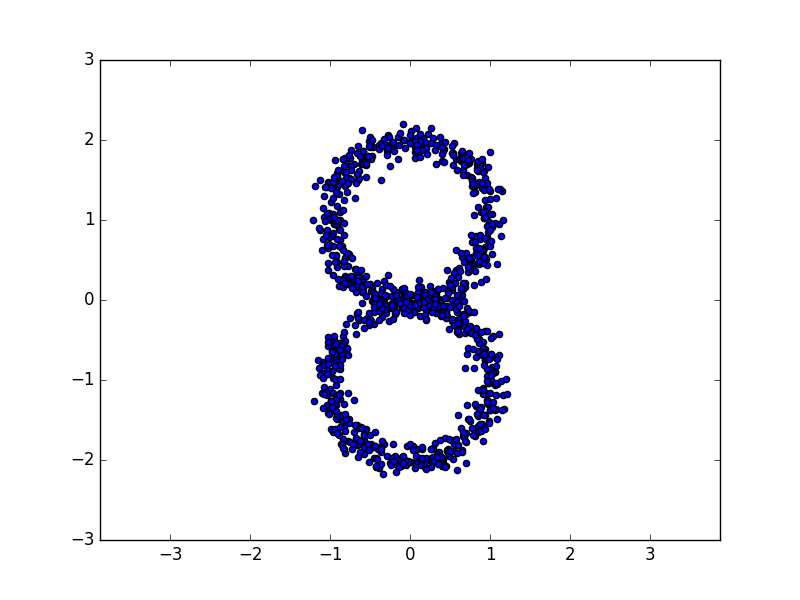
\includegraphics[scale=0.40]{img/s1vs1.png}
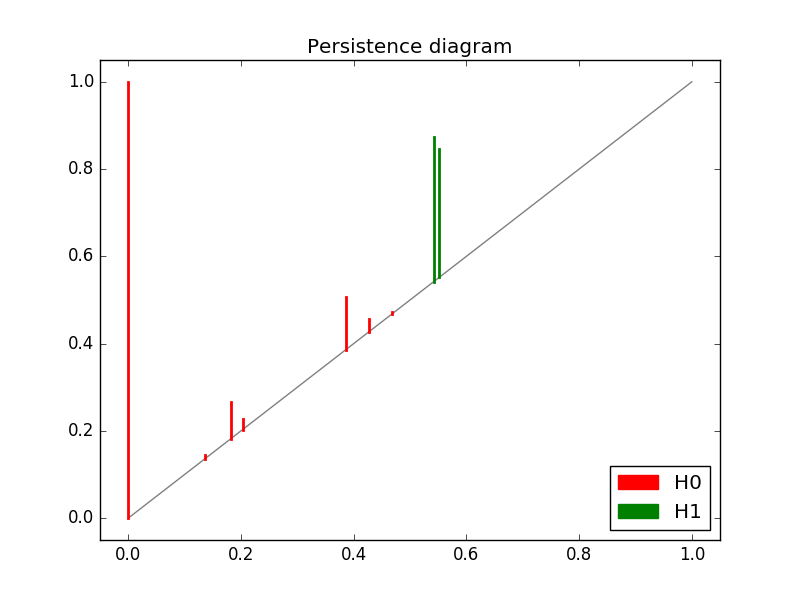
\includegraphics[scale=0.40]{img/cubex_diagram.png}
\caption{Nube de datos y su diagrama de persistencia.}
\label{diagram_cubex}
\end{figure}

La Figura \ref{diagram_cubex} muestra otro ejemplo de diagrama de persistencia, éste hecho con el módulo \texttt{Cubix} que se desarrolla en este trabajo. La filtración que se ha hecho en este ejemplo es la filtración por KDE que se desarrolla aquí. En el diagrama pueden verse con claridad dos líneas verdes y una roja que se alejan de la diagonal. Las dos líneas verdes nos hablan de los dos agujeros de dimensión 1 que se pueden apreciar en la nube de datos ($H_1=\F_2^2$), mientras que la roja nos habla de que tiene una única componente conexa ($H_0=\F_2$).

\subsubsection{Códigos de barras}
En \cite{Carlsson}, Gunnar Carlsson propone este nuevo formato para representar los resultados. En estos diagramas se dibuja una línea horizontal por cada generador de persistencia $g$ que va desde la abscisa $\tau_B(g)$ hasta la abscisa $\tau_D(g)$. Cada barra se representa a una altura diferente, comenzando desde abajo, y por lo general se realiza un gráfico diferente para cada dimensión.

\begin{figure}[h!]
\centering
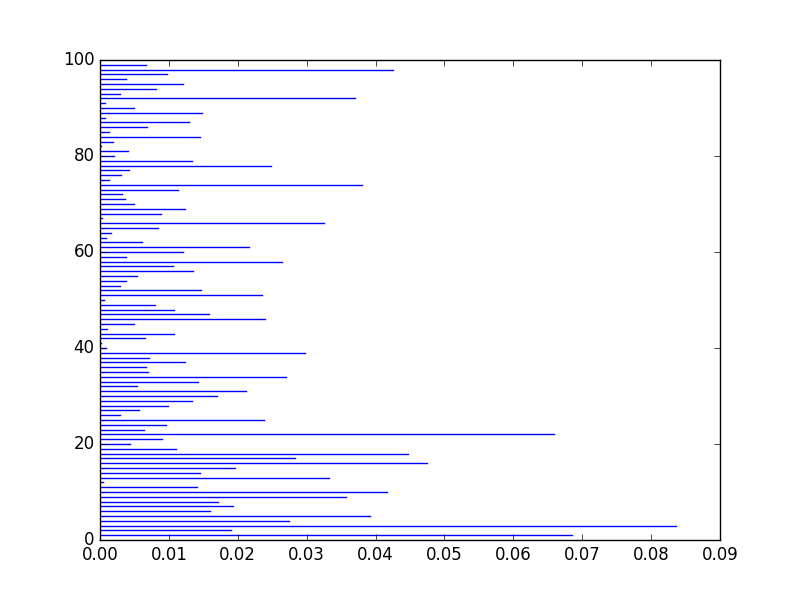
\includegraphics[scale=0.33]{img/bars0.png}
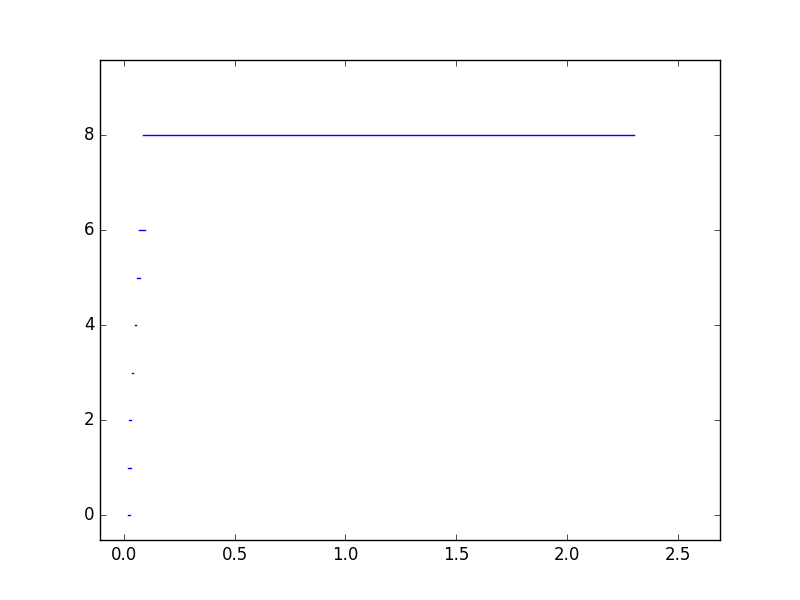
\includegraphics[scale=0.33]{img/bars.png}
\caption{Códigos de barras de la filtración de la Figura \ref{filtracion}.}
\label{barras}
\end{figure}

La Figura \ref{barras} muestra los códigos de barras de la misma filtración de la Figura \ref{filtracion}, realizados también con la herramienta \texttt{Dionysus}. Al igual que en el Figura \ref{diagramas}, la gráfica de la izquierda corresponde a dimensión 0 y la segunda a dimensión 1. El análisis que uno hace es esencialmente el mismo: en dimensión 1 vemos una única barra que muestra una larga persistencia, mientras que en la de la izquierda son todas barras cortas. Se estima entonces $H_0=0$ y $H_1=\F_2$, i.e., la homología de $S^1$.



\newpage
\section{Homología cúbica simplicial}

% --------------------------------
%
% SECCIÓN 3: HOMOLOGÍA CÚBICA SIMPLICIAL
%
% --------------------------------

El complejo sobre el que definimos nuestra filtración está formado por $m$-cubos ---puntos, segmentos, cuadrados, cubos e hipercubos en general--- y por ello no se trata de un complejo simplicial tal como habitualmente los conocíamos (como se definen en \cite{Navarro}). Ésto no supone un problema si se definen estos cubos de una forma rigurosa y con ellos se llega a construir un complejo de cadenas con una diferencial $\partial$ que cumpla $\partial^2=0$. En \cite{Massey}, W. Massey hace una primera formalización del concepto de \emph{$m$-símplex cúbico} como aplicación continua del $m$-cubo estándar sobre un espacio topológico $X$, que ha sido utilizada por diversos autores en otras ramas de la topología.

En nuestro caso, el complejo con el que vamos a lidiar es bastante simple por el hecho de estar formado de puntos equidistantes sobre una cuadrícula en el espacio euclídeo. No queremos alejarnos del problema que nos ocupa, y por ello nos apoyaremos bastante en esta simetría que ofrece el complejo y definiremos una noción bastante particular de \emph{cubo simplicial} (similar al concepto de símplex) que nos ayudará a formular de una forma sencilla y explícita toda la teoría de homología.

\subsection{Cubos simpliciales}

Los $m$-cubos que forman el complejo de nuestra filtración tienen todos el mismo costado $\varepsilon$ (la precisión de la cuadrícula) y se extienden únicamente en las direcciones canónicas de $\R^n$. Fijado $\varepsilon > 0$, todo $m$-cubo de la filtración se puede determinar de forma unívoca por un punto raíz $P\in \R^n$ y un conjunto de $m$ direcciones en las que se expande dicho punto para formar el $m$-cubo.

\begin{definicion}
Fijamos $\varepsilon > 0$. Sea $P=(x_1,\dots,x_n)\in\R^n$ y $D=\{d_1,\dots,d_m\}$ un conjunto ordenado de $m$ enteros distintos $1\leq d_1 < \dots <d_m \leq n$. Considérese el conjunto de puntos
$$ \Pi_{\varepsilon,P,D} = \lbrace P + \sum_{i\in\sigma} \delta_i  \in \R^n  \tq \sigma \in \mathcal{P}(D) \rbrace $$
donde $\mathcal{P}(D)$ es el conjunto potencia de $D$ y $\delta_i = \varepsilon e_i$ es un aumento de $\varepsilon$ en la coordenada $i$. Definimos el \emph{$m$-cubo simplicial} de costado $\varepsilon$ con raíz en $P$ y direcciones $D$ ---que denotamos $\Gamma = \Gamma_{\varepsilon,P,D}$--- como la envolvente convexa del conjunto $\Pi_{\varepsilon,P,D}$. Decimos que $\Pi(\Gamma) = \Pi_{\varepsilon,P,D}$ son los \emph{vértices} (o \emph{puntos}) del cubo. Definimos la \emph{dimensión} del cubo simplicial como $m=\vert D\vert$.
\end{definicion}

\begin{notacion}
Dado que $\varepsilon$ será siempre el mismo fijado para todos los $m$-cubos de los que hablaremos, omitiremos, siempre que no haya posibilidad a confusión, el subíndice $\varepsilon$ para denotar $\Gamma_{P,D} = \Gamma_{\varepsilon,P,D}$.
\end{notacion}

La definición puede parecer algo complicada, pero lo único que se hace es construir a partir de $P$ el conjunto de todos los vértices del $m$-cubo sumando $\varepsilon$ sobre las coordenadas correspondientes dictadas por $D$. A continuación se muestran algunos ejemplos que ayudan a entender el $m$-cubo que se forma de una raíz y un conjunto de direcciones. Nótese que, por su propia definición, un $m$-cubo tiene $2^m$ vértices (como bien es sabido) ya que estos se forman a partir del conjunto potencia de $D$, que tiene $m$ elementos.

\begin{figure}[h]
\centering
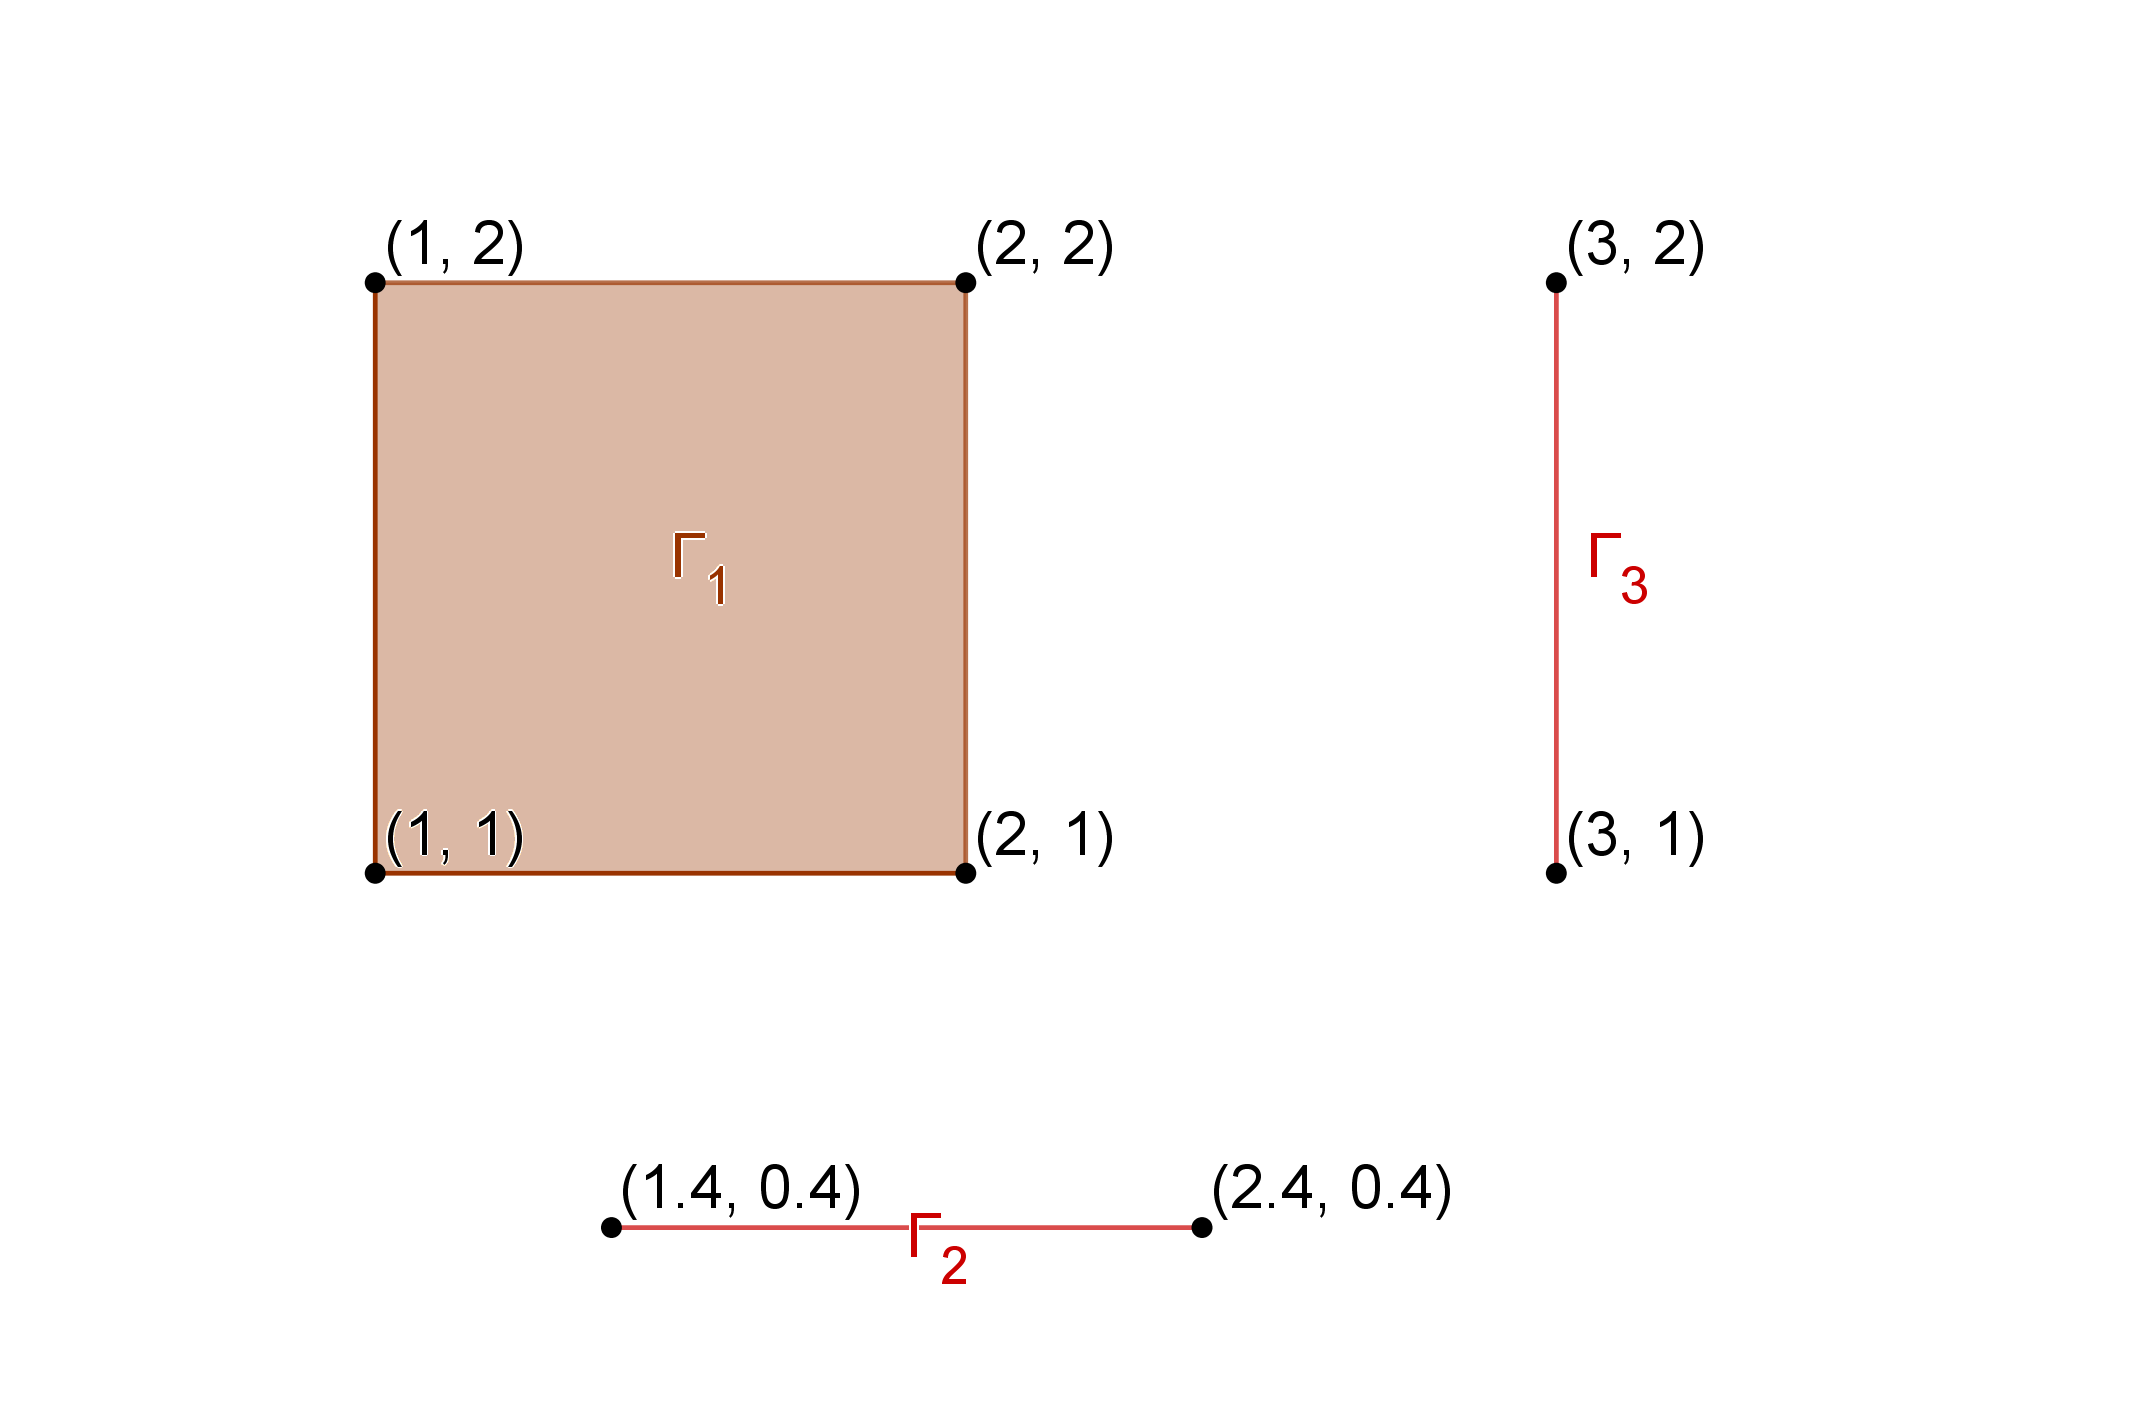
\includegraphics[scale=0.6]{img/cubos.png}
\caption{Ejemplos de cubos en $\R^2$.}
\label{cubos}
\end{figure}

\begin{ejemplo}
A continuación se muestran algunos ejemplos de $m$-cubos:
\begin{enumerate}[(i)]
\item Si tomamos $P=(1,1)\in\R^2$ y direcciones $D= \{ 1,2 \}$ (las dos direcciones posibles de $\R^2$) y costado $\varepsilon = 1$ entonces $\Gamma_{P,D}$ es el $2$-cubo ---cuadrado--- formado por los puntos $(1,1)$, $(1,2)$, $(2,1)$ y $(2,2)$. En la Figura \ref{cubos} podemos ver este cubo etiquetado con $\Gamma_1$. 
\item En la Figura \ref{cubos} también tenemos ejemplos de $1$-cubos ---segmentos--- en $\R^2$. El segmento etiquetado con $\Gamma_2$ es el cubo formado por un punto $P=(1.4,0.4)\in \R^2$ y con una única dirección, la horizontal, i.e., $D= \{ 1\}$. El segmento etiquetado con $\Gamma_3$ se construye a partir del punto $P=(3,1)\in\R^2$ con dirección $D= \{ 2\}$. En ambos seguimos usando $\varepsilon = 1$.
\item Un $0$-cubo se forma cuando $D= \emptyset$. En tal caso el cubo se corresponde a un único punto.
\item En la Figura \ref{cubos3d} se muestran un par de ejemplos de 2-cubos en $\R^3$, en ambos el punto raíz es $P=(0,0,0)\in \R^3$ y la distancia $\varepsilon=1$. El que etiquetamos con $\Gamma_4$ tiene direcciones $D= \{2,3 \}$ mientras que el tiene etiqueta $\Gamma_5$ tiene direcciones $D= \{1,2 \}$.
\end{enumerate}
\end{ejemplo}


\begin{figure}[h]
\centering
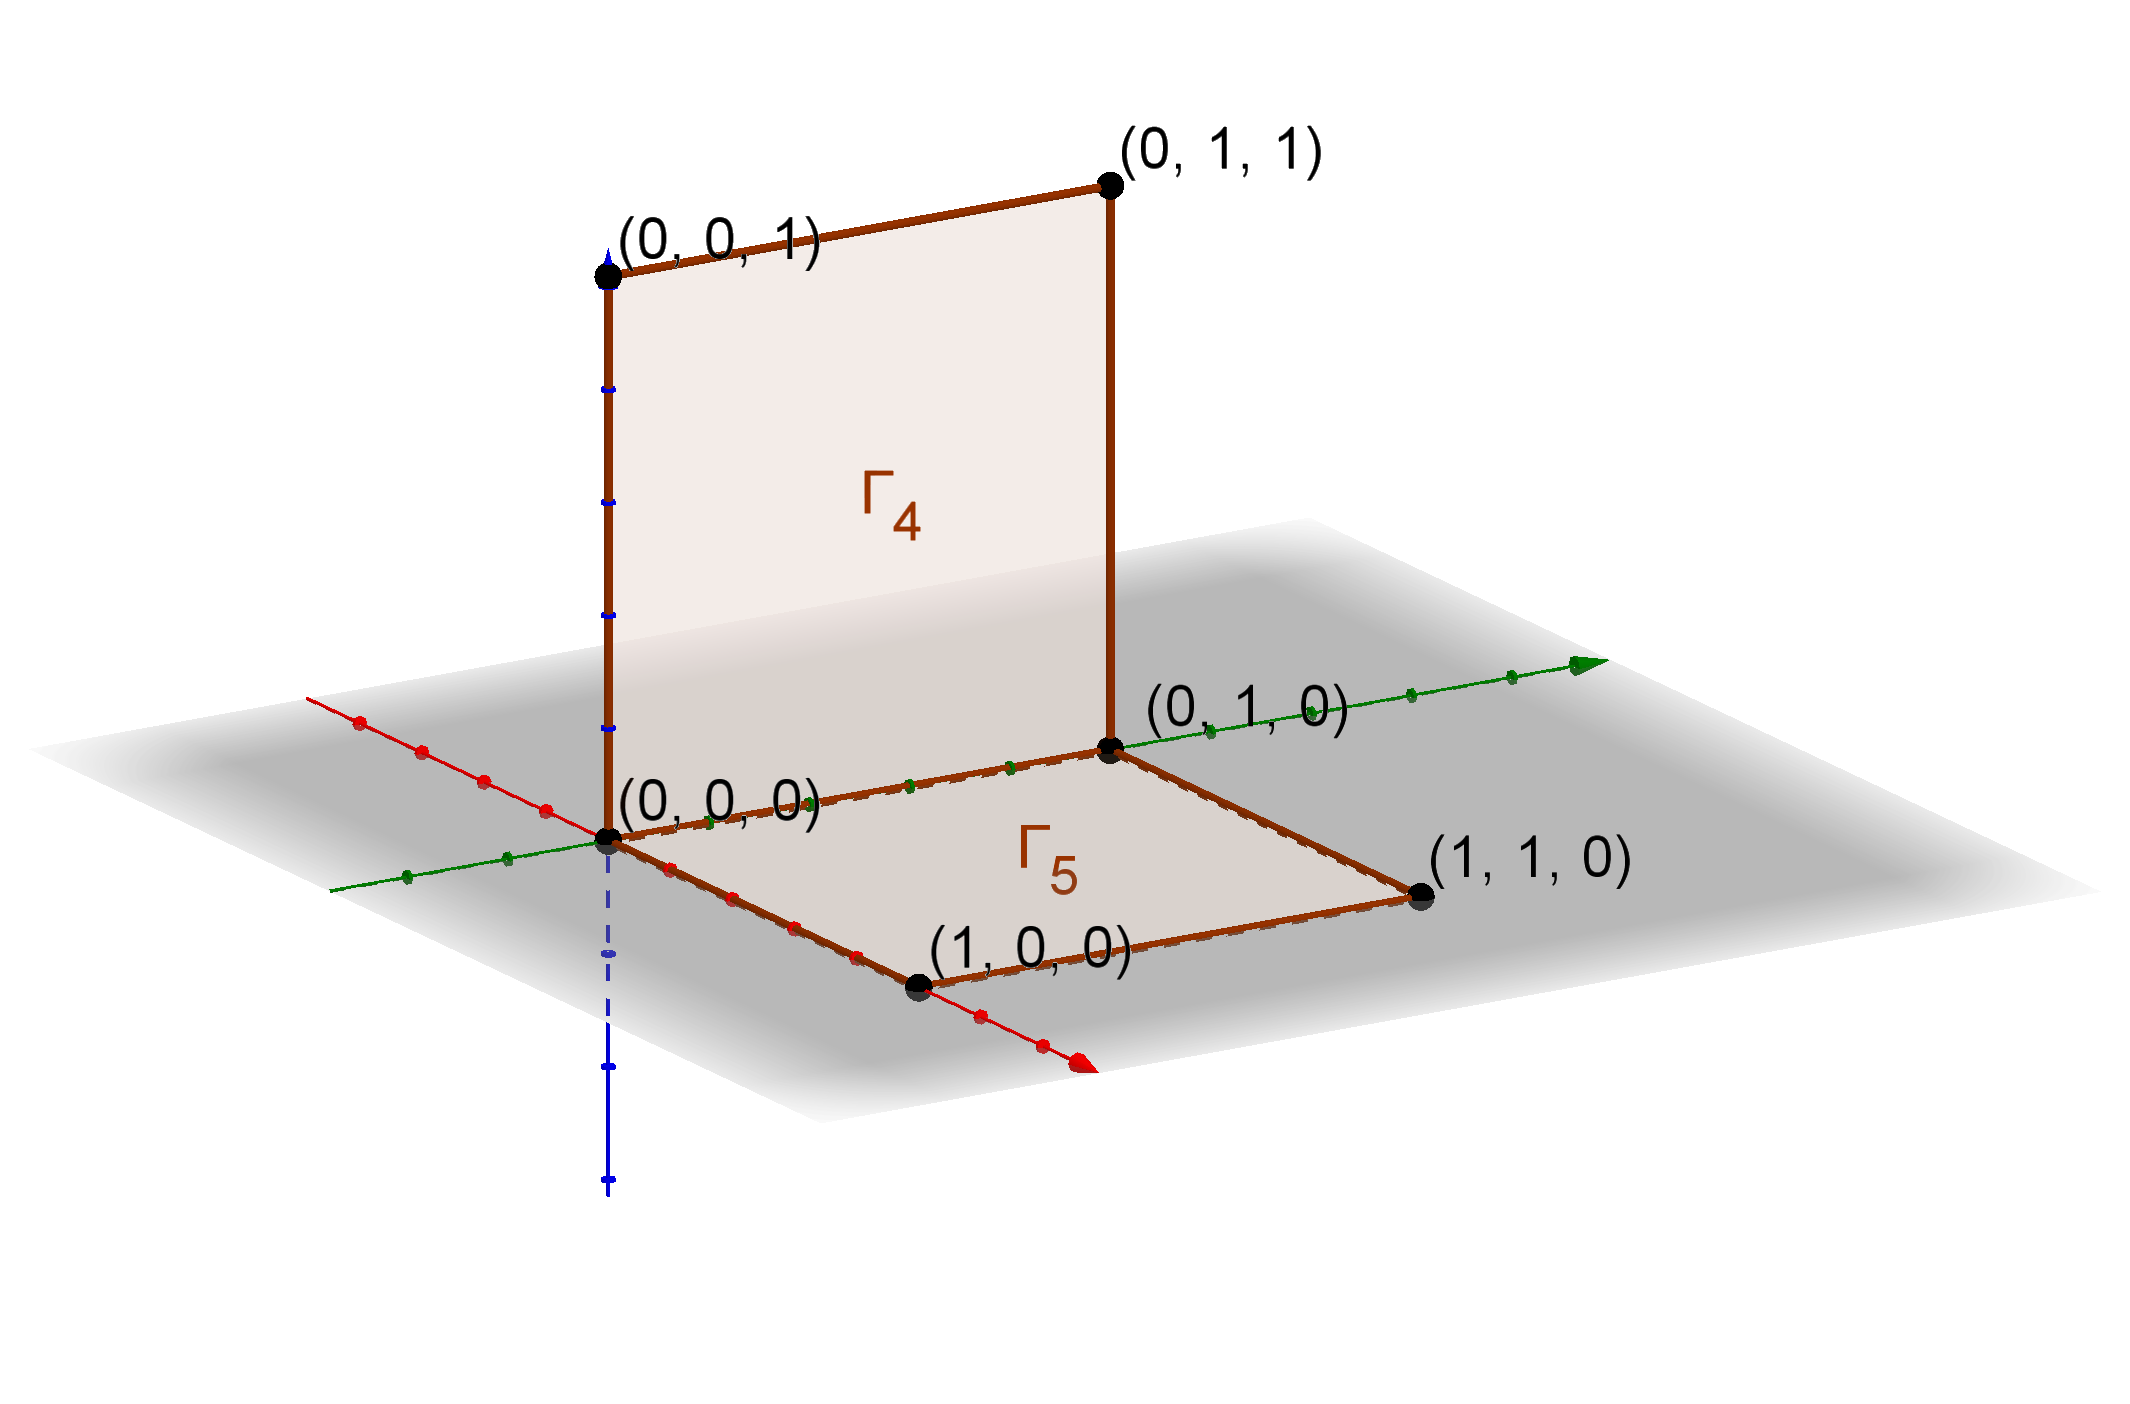
\includegraphics[scale=0.6]{img/cubos3d.png}
\caption{Ejemplos de cubos en $\R^3$.}
\label{cubos3d}
\end{figure}

\subsection{Complejos cúbicos}

Para poder construir una teoría de homología será necesario hablar de complejos simpliciales, y para definirlos se necesita una noción de \emph{caras} para nuestros $m$-cubos. En un símplex común las caras $k$-dimensionales no son más que los símplices formados por $(k+1)$-puntos de éste. A priori no parece complicado pensar en las caras de un $m$-cubo, pero su definición formal como cubos simpliciales de dimensión inferior requiere algo de esfuerzo en la notación.

\begin{definicion}
Sea $\Gamma = \Gamma_{P,D}$ un cubo simplicial de dimensión $m\geq1$ con raíz $P=(x_1,\dots,x_n)\in\R^n$ y direcciones $D=\{d_1,\dots,d_m\}$. Definimos el conjunto de \emph{caras} de $\Gamma$ como
$$ C(\Gamma) = \lbrace \Gamma_{P,\hat{D}_i} \rbrace_{i=0,\dots,m} \cup \lbrace \Gamma_{P+\delta_{d_i},\hat{D}_i}\rbrace_{i=0,\dots,m}  $$
donde usamos la notación $\hat{D}_i = D\backslash\{d_i\}$. Esto es, las caras de $\Gamma$ son símplices que tienen las mismas direcciones que $\Gamma$ salvo una, y que tienen como raíz el propio $P$ o el punto $P$ trasladado $\varepsilon$ en la misma dirección que se haya quitado. Si $\Gamma$ es un cubo simplicial de dimensión 0 el conjunto de caras es vacío.
\end{definicion}

\begin{ejemplo}
Veamos un ejemplo concreto de cómo se construyen las caras de un $m$-cubo. Considérese el $2$-cubo con raíz $P=(1,1)\in\R^2$, direcciones $D=\{1,2\}$ y $\varepsilon = 1$ (cuadrado con etiqueta $\Gamma_1$ de la Figura \ref{cubos}). Sus caras son los siguientes cuatro $1$-cubos:
\begin{itemize}
\item El cubo con raíz en $P=(1,1)$ y dirección $D=\{1\}$.
\item El cubo con raíz en $P=(1,1)$ y dirección $D=\{2\}$.
\item El cubo con raíz en $P=(2,1)$ y dirección $D=\{2\}$.
\item El cubo con raíz en $P=(1,2)$ y dirección $D=\{1\}$.
\end{itemize}
Véase en la Figura \ref{cubos} que estos cuatro $1$-cubos corresponden a los segmentos que delimitan el cuadrado.
\label{carascuadrado}
\end{ejemplo}

Nótese que un $m$-cubo tiene $2m$ caras (un segmento tiene 2 vértices, un cuadrado tiene 4 costados, un cubo 6 caras...), dos por cada dirección que se puede quitar. La noción de caras de dimensiones inferiores puede extenderse por inducción de esta definición, i.e., definimos las caras $(m-2)$-dimensionales de un $m$-cubo el conjunto de caras de las caras de éste, y así sucesivamente.

La definición de complejo cúbico simplicial es una extensión directa de la noción de complejo simplicial.

\begin{definicion}
Definimos un \emph{complejo cúbico simplicial} $K$ ---o sencillamente \emph{complejo cúbico}--- como una colección de complejos cúbicos tal que:
\begin{enumerate}
\item Si $\Gamma \in K$ y $\sigma$ es una cara de $\Gamma$, entonces $\sigma \in K$.
\item Si $\Gamma,\Gamma' \in K$, $\Gamma \neq \Gamma'$, con $\Gamma \cap \Gamma' \neq \emptyset$, entonces $\Gamma \cap \Gamma'$ es una cara de $\Gamma$ y de $\Gamma'$.
\end{enumerate}
\end{definicion}

\begin{definicion}
Definimos la \emph{realización geométrica} un complejo cúbico simplicial $K$ como el subespacio de $\R^n$ formado por los símplices del complejo, i.e.:
$$ \lvert K \rvert = \bigcup_{\Gamma \in K} \Gamma \subset \R^n$$ 
\end{definicion}

\begin{definicion}
Sea $K$ un complejo cúbico simplicial. Decimos que un subconjunto $K' \subset K$ es un \emph{subcomplejo} de $K$ si $K'$ es a su vez un complejo cúbico simplicial.
\end{definicion}

\begin{definicion}
Dado un complejo cúbico simplicial $K$ finito, definimos una \emph{filtración} sobre $K$ como una familia de subcomplejos $\mathcal{F} = \lbrace K_i \subseteq K \rbrace_{i \in I}$ indexados sobre un conjunto ordenado $I$ tal que si $i<j$ entonces $K_i \subseteq K_j$, y además $\emptyset,K \in \mathcal{F}$.
\end{definicion}

\subsection{Frontera y morfismos diferenciales}

Definiremos a continuación el concepto de \emph{frontera} de un cubo simplicial. En homología simplicial, la frontera no es más que una cierta suma formal de las caras de un símplice. Para poder hablar de este tipo de sumas de caras es necesario tomar un anillo $R$ y considerar el $R$-módulo generado por éstas. A lo largo de esta sección, $R$ será un anillo conmutativo y con unidad. Referencias al concepto de $R$-módulo y álgebra conmutativa en general pueden encontrarse en \cite{Atiyah}.

\begin{definicion}
Sea $K$ un complejo cúbico simplicial. Para todo $p\geq0$ se define el \emph{grupo de cadenas $p$-dimensionales} de $K$, que denotamos por $Q_p(K; R)$ ---o sencillamente $Q_p(K)$---, al $R$-módulo libre generado por los $p$-cubos del complejo $K$.
\end{definicion}

\begin{definicion}
Sea $\Gamma = \Gamma_{P,D}$ un cubo simplicial de dimensión $m$ de un complejo cúbico $K$ y sean $d_1,\dots,d_m \in D$ las direcciones del cubo ordenadas de menor a mayor. Definimos la \emph{frontera} de $\Gamma$ como la suma
$$ \partial(\Gamma) :=  \sum_{k=1}^m (-1)^{k}\Gamma_{P,\hat{D}_k} - \sum_{k=1}^m (-1)^{k}\Gamma_{P+\delta_{d_k},\hat{D}_k} \in Q_{m-1}(K)$$
\end{definicion}

\begin{observacion}
Nótese que la frontera de un $m$-cubo no deja de ser una suma alternada de las caras de éste, y está bien definido ya que toda cara de $\Gamma$ forma parte del complejo $K$ y tiene dimensión $m-1$. Véase además que para el caso de $R=\mathbb{F}_2$, donde $-1=1$, la frontera del cubo puede escribirse sencillamente como $\partial_p(\Gamma) = \sum_{\sigma\in C(\Gamma)} \sigma$.
\end{observacion}

\begin{ejemplo}
Poniendo los signos de esta forma se obtiene una frontera que se asemeja mucho a la de la homología simplicial común. Veamos algunos ejemplos calculando explícitamente la frontera:
\begin{enumerate}[(i)]
\item El cuadrado con etiqueta $\Gamma_1$ de la Figura \ref{cubos} se escribe $ \Gamma_{(1,1),\{1,2\}}$ como $2$-cubo. Su frontera sería
\begin{align*}
\partial \left( \Gamma_{(1,1),\{ 1,2 \}} \right) &= - \Gamma_{(1,1),\{ 2 \}} + \Gamma_{(1,1),\{ 1 \}} +  \Gamma_{(2,1),\{ 2 \}} - \Gamma_{(1,2),\{ 1 \}} \\
&= \Gamma_{(1,1),\{ 1 \}} + \Gamma_{(2,1),\{ 2 \}} - \Gamma_{(2,1),\{ 2 \}} - \Gamma_{(1,1),\{ 2 \}}
\end{align*}
Las caras que aparecen se corresponden con los segmentos que delimitan el cuadrado, tal como habíamos visto en el Ejemplo \ref{carascuadrado}. Nótese que escrito de la segunda manera puede entenderse como si recorriéramos los costados del cuadrado en sentido antihorario, tal como sucede con la frontera de un símplex.

\item En el caso de un $1$-cubo como $\Gamma_{(3,1),\{2\}}$ (etiquetado con $\Gamma_3$ en la Figura \ref{cubos}), la frontera quedaría
$$ \partial \left( \Gamma_{(3,1),\{ 2 \}} \right) = - \Gamma_{(3,1),\emptyset} + \Gamma_{(3,2),\emptyset} $$
que, dicho de otra forma, es el ``punto final'' menos el ``punto inicial'', exactamente igual que en el caso de un $1$-símplex.
\end{enumerate}
\end{ejemplo}

La frontera de un $m$-cubo puede extenderse a un morfismo de $R$-módulos entre los grupos de cadenas $m$-dimensionales y $(m-1)$-dimensionales, y ésto es lo que llamamos el morfismo \emph{diferencial}.

\begin{definicion}
Sea $K$ un complejo cúbico simplicial. Para todo $p\geq 0$, se define el \emph{morfismo diferencial} $\map{\partial_p}{Q_p(K)}{Q_{p-1}(K)}$ que actúa sobre los generadores $\Gamma \in Q_p(K)$ de la forma $\partial_p(\Gamma) = \partial(\Gamma)$.
\end{definicion}


\begin{proposicion}
Sea $K$ un complejo simplicial y $R$ un anillo conmutativo con identidad. La composición
$$ Q_{p+1}(K) \stackrel{\partial_{p+1}}{\longrightarrow} Q_p(K) \stackrel{\partial_p}{\longrightarrow} Q_{p-1}(K) $$
es nula para todo $p\geq 1$, i.e., $\partial_p \circ \partial_{p+1} = 0$.
\end{proposicion}

\begin{proof}
Basta con demostrarlo para un generador de $Q_{p+1}(K)$. Tomamos $\Gamma_{P,D}$ con $d_1,\dots,d_{p+1} \in D$ las direcciones de éste ordenadas.

Por linealidad, se tiene:
\begin{align*}
\partial_p(\partial_{p+1}(\Gamma_{P,D})) &= \partial_p \left( \sum_{k=1}^{p+1} (-1)^{k}\Gamma_{P,\hat{D}_k} - \sum_{k=1}^{p+1} (-1)^{k}\Gamma_{P+\delta_{d_k},\hat{D}_k} \right) \\
                                   &= \sum_{k=1}^{p+1} (-1)^{k} \partial_p \left( \Gamma_{P,\hat{D}_k} \right) - \sum_{k=1}^{p+1} (-1)^{k}\partial_p \left( \Gamma_{P+\delta_{d_k},\hat{D}_k} \right)
\end{align*}

Las diferenciales $\partial_p ( \Gamma_{P,\hat{D}_k} )$ y $\partial_p ( \Gamma_{P+\delta_{d_k},\hat{D}_k} )$ consisten ambas en sumas alternadas extrayendo en orden las direcciones de $\hat{D}_k$. Obsérvese que el elemento $d_l \in D$ ocupa la posición $l$ en $\hat{D}_k$ si $l < k$, y la posición $l-1$ cuando $l > k$, y por tanto aparecerá con signo contrario en uno y otro caso. 

En la suma total aparecen, por cada par de direcciones $d_i,d_j \in D$, cuatro $m$-cubos con direcciones $\hat{D}_{i,j}=D \backslash \{d_i,d_j\}$, que son:
$$\Gamma_{P,\hat{D}_{i,j}} , \, \Gamma_{P+\delta_{d_i},\hat{D}_{i,j}} , \, \Gamma_{P+\delta_{d_j},
\hat{D}_{i,j}} , \, \Gamma_{P+\delta_{d_i}+\delta_{d_j},\hat{D}_{i,j}}$$

Todos estos aparecen por duplicado: una vez cuando se extrae $d_i$ en la primera diferencial y $d_j$ en la segunda, y otra cuando se extrae primero $d_j$ y luego $d_i$. Si suponemos, sin pérdida de generalidad, que $i > j$, en el primer caso aparecerán con signo $(-1)^i\cdot (-1)^j$, mientras que en el segundo, que $d_i$ ocupa la posición $j-1$ de $\hat{D}_j$, el signo con el que aparecerán será $(-1)^j\cdot(-1)^{i-1}$, y por tanto se cancelan mútuamente.
\end{proof}

\subsection{Grupos de homología de un complejo cúbico}

Dado que los morfismos $\partial_p$ cumplen $\partial_p \circ \partial_{p+1} = 0$ para todo $p \geq 0$, se puede construir con ellos un complejo de $R$-módulos
$$ \cdots \longrightarrow Q_{p+1}(K) \stackrel{\partial_{p+1}}{\longrightarrow} Q_p(K) \stackrel{\partial_p}{\longrightarrow} Q_{p-1}(K) \cdots \stackrel{\partial_1}{\longrightarrow} Q_0(K) \stackrel{\partial_0}{\longrightarrow} 0 $$
sobre el que definir los grupos de homología, que denotaremos por $Q_*(K)$.

\begin{definicion}
Sea $K$ un complejo cúbico simplicial y sean $\partial_i$ con $i\geq0$ los morfismos diferenciales del complejo de $R$-módulos generado por $K$. Para todo $p\geq 0$ definimos el \emph{$p$-ésimo grupo de homología cúbica de $K$ sobre $R$} como \footnote{Éstos grupos de homología dependen del anillo $R$ que se tome. En caso de ser necesario especificar dicho anillo escribiríamos $H_p(K;R)$.}
$$ H_p(K) =  H_p(Q_*(K)) = \quotient{\ker{\partial_p}}{\Img{\partial_{p+1}}}$$
\end{definicion}

Será útil también definir el concepto de \emph{homología relativa}. Si $L \subset K$ es un subcomplejo de $K$, el complejo $Q_*(L)$ se inyecta en $Q_*(K)$ de forma que podemos hablar del complejo cociente de estos dos.

\begin{definicion}
Sea $K$ un complejo cúbico simplicial y $L \subset K$ un subcomplejo de éste. Definimos el \emph{$p$-ésimo grupo de homología del par $(K,L)$} como el $p$-ésimo grupo de homología del complejo $\quotient{Q_*(K)}{Q_*(L)}$, y lo denotaremos $H_p(K,L)$.
\end{definicion}

\subsection{Equivalencia de la homología cúbica}

Hasta aquí tenemos definida una homología sobre el complejo cúbico $K$. Veremos ahora que esta homología coincide con la de un complejo simplicial $K^T$ que represente el mismo subespacio de $\R^n$, i.e., que tenga la misma realización geométrica. Para ello necesitamos \emph{triangular} los cubos del complejo $K$.

\subsubsection{Triangulación del $m$-cubo}
Sea $\Gamma = \Gamma_{P,D}$ un $m$-cubo con $P\in\R^n$ y $D=\{d_1,\dots,d_m\}$. Sea $S_m$ el grupo de permutaciones de $m$ elementos. Para cada $\sigma \in S_m$, considérense los $m+1$ puntos
$$P, P+\delta_{d_{\sigma(1)}}, P+\delta_{d_{\sigma(1)}}+\delta_{d_{\sigma(2)}},\dots,P+\delta_{d_{\sigma(1)}}+\cdots+\delta_{d_{\sigma(m)}}$$
los cuales son afínmente independientes y definen por tanto (en este orden) un $m$-símplex que denotaremos por $\Delta_\sigma(\Gamma)$. Nótese que los puntos que definen $\Delta_\sigma(\Gamma)$ son un subconjunto de los que definen $\Gamma$, y por ello se tiene la inclusión de envolventes convexas $\Delta_\sigma(\Gamma) \subset \Gamma$, para todo $\sigma \in S_m$. Éstos son los símplices con los que triangularemos nuestro $m$-cubo.

\begin{observacion}
Obsérvese que el punto raíz $P$ y el punto opuesto $P+\sum_{d\ in D}\delta_d$ forman parte de todos los símplices $\Delta_\sigma$ de la triangulación. Los puntos de cada símplex $\Delta_\sigma$ son las distintos \emph{caminos} para llegar del punto raíz al punto opuesto aumentando de a una cada coordenada.  Si $\Gamma$ es un $0$-cubo ($D=\emptyset$), la triangulación consiste en un único símplex que es el propio punto $P$, como $0$-símplex.
\end{observacion}

\begin{notacion}
Abusando un poco de notación, escribiremos estos símplices como $\Delta_\sigma(\Gamma)=[\sigma_0,\dots,\sigma_m]$ con $\sigma_0=P$ y $\sigma_k=P+\sum_{i=1}^k\delta_{\sigma(i)}$ para $k=1,\dots,m$.
\end{notacion}

\begin{figure}[h!]
\centering
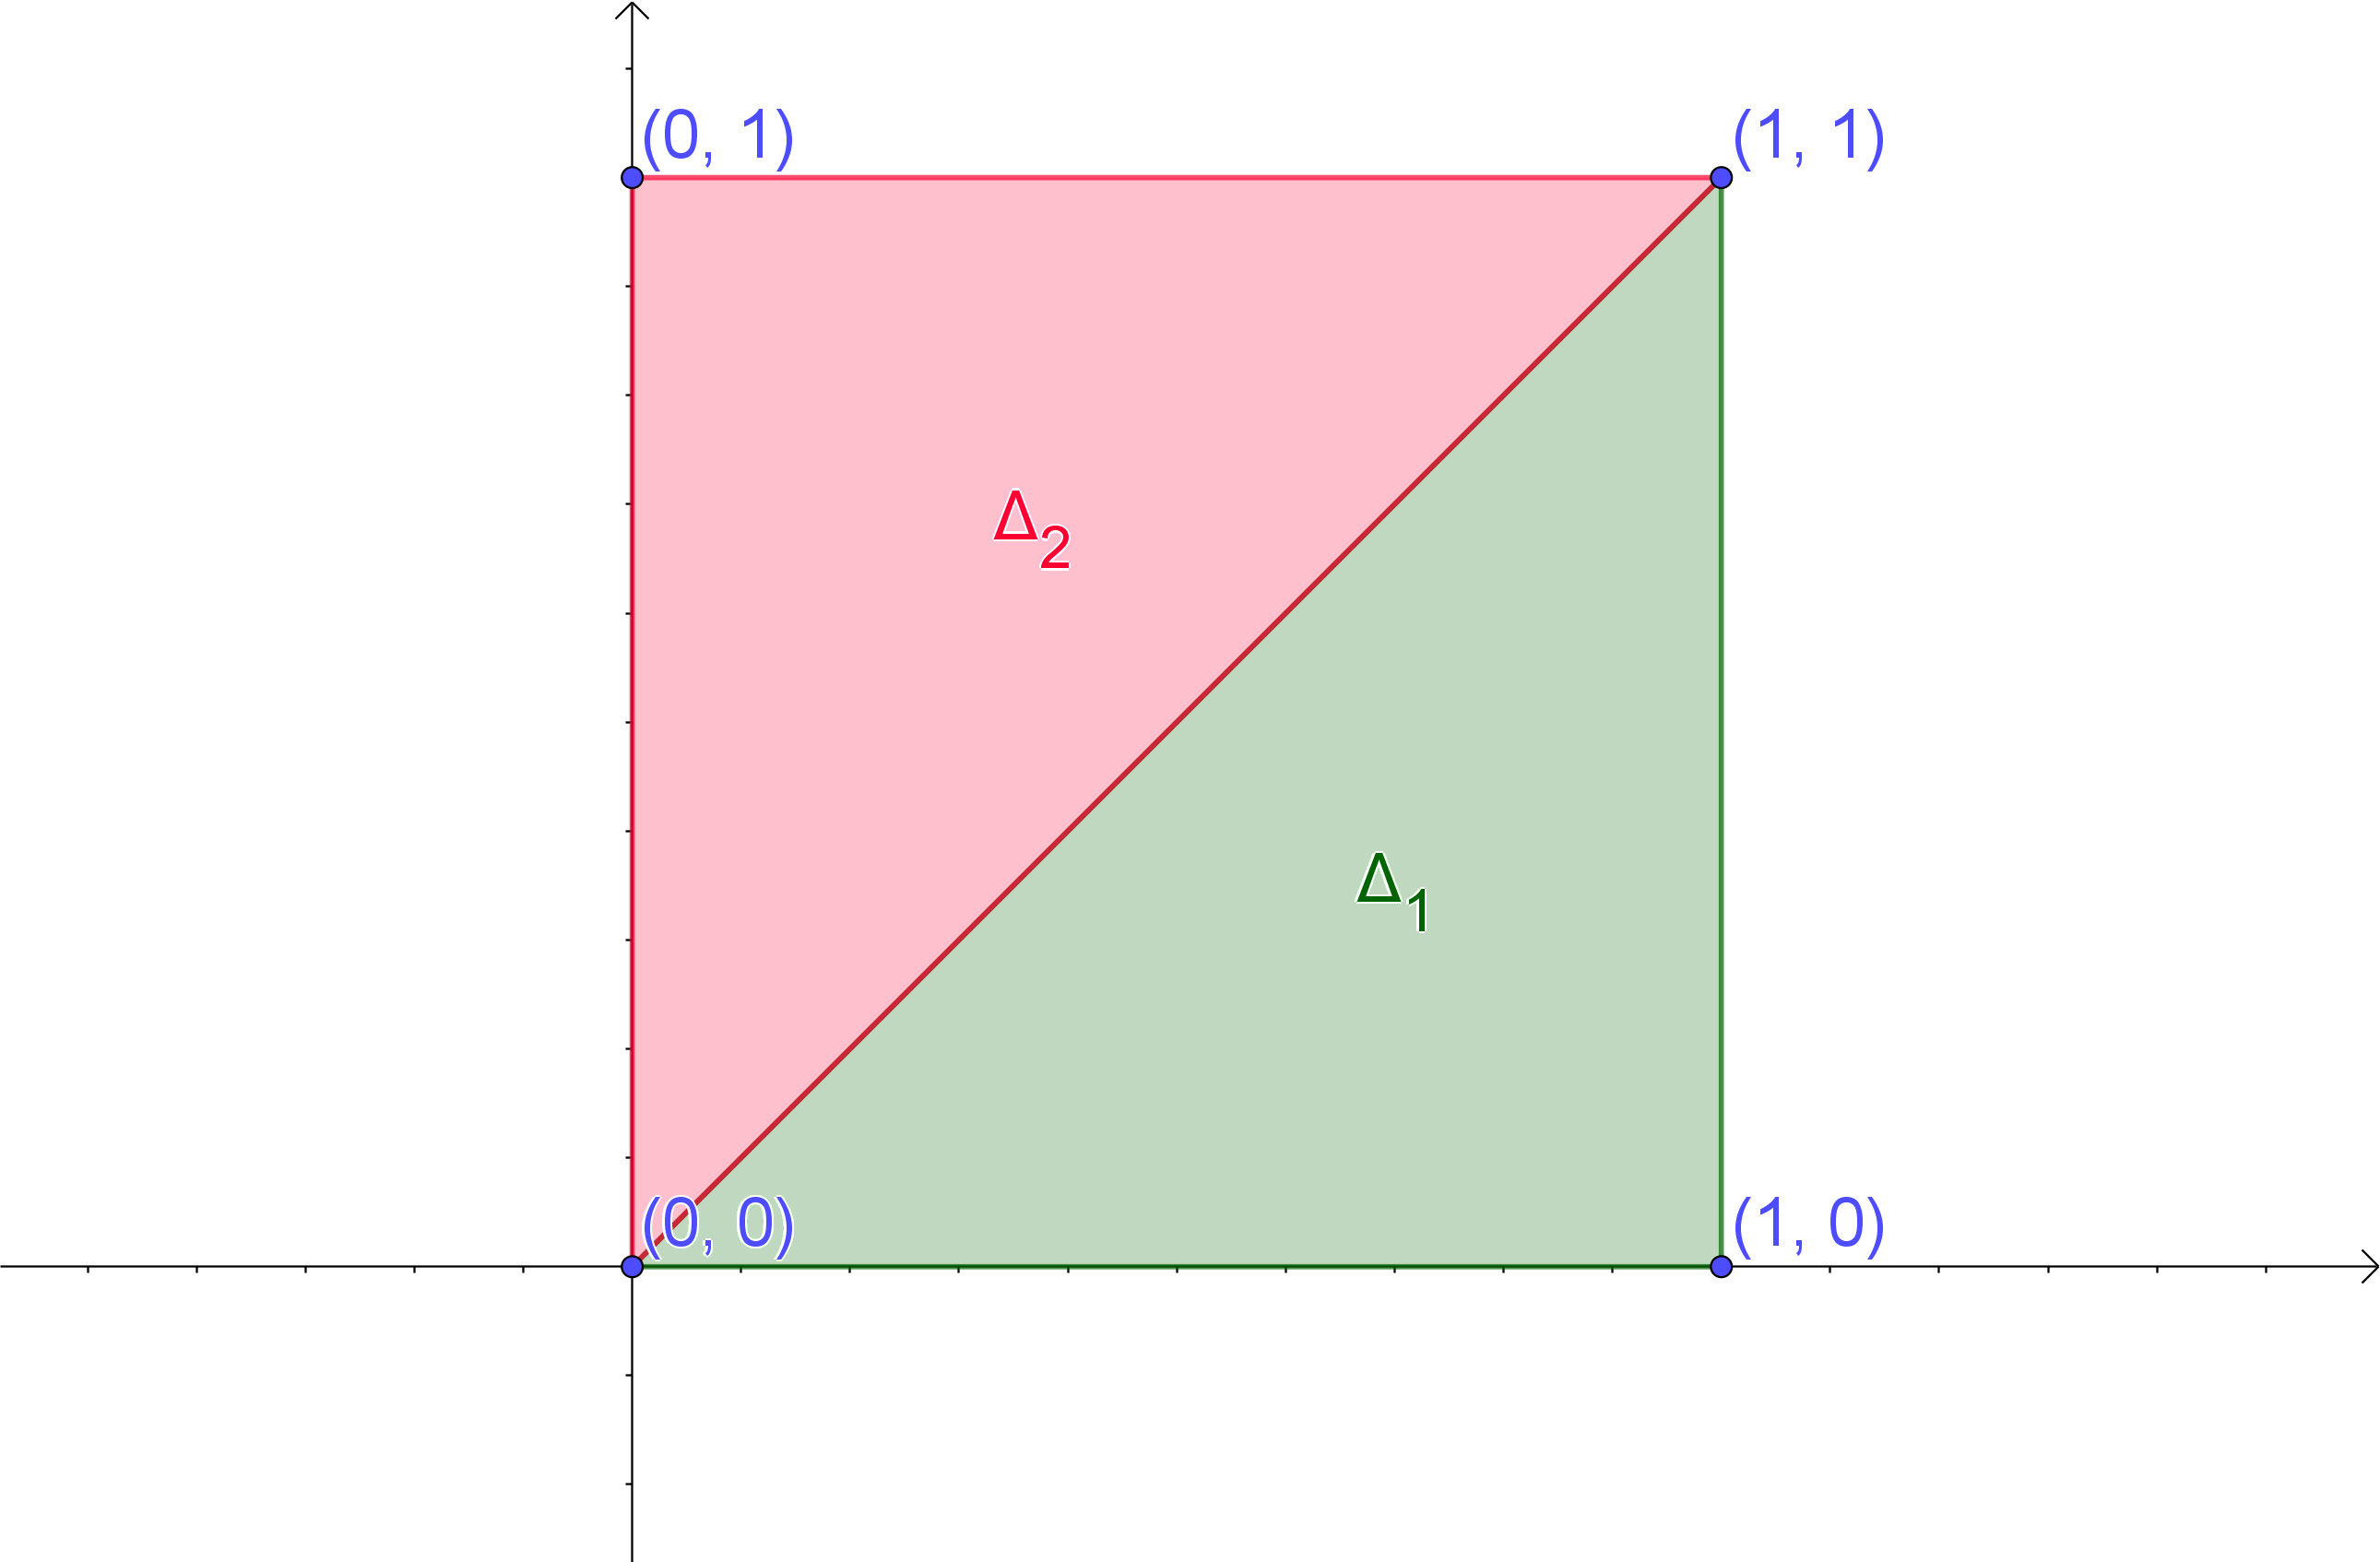
\includegraphics[scale=0.40]{img/triangulacioncuadrado.png}
\caption{Triangulación del $2$-cubo estándar de $\R^2$.}
\label{triangulacioncuadrado}
\end{figure}

\begin{ejemplo}
Nuevamente la notación es algo compleja, por ello exponemos un par de ejemplos explícitos de triangulación (en ambos se toma $\varepsilon=1$):
\begin{enumerate}[(i)]
\item Si $\Gamma = \Gamma_{(0,0),\{1,2\}} \subset \R^2$, la triangulación consiste en dos símplices, correspondientes a los dos elementos de $S_2$ (véase la Figura \ref{triangulacioncuadrado}):
\begin{itemize}
\item Para la permutación identidad, se aumenta primero la primera coordenada y luego la segunda, resultando el símplex $[(0,0),(1,0),(1,1)]$.
\item El otro símplex, dado por la trasposición $(1,2)\in S^2$, se forma aumentando primero la segunda coordenada y luego la primera, obteniéndose el símplex $[(0,0),(0,1),(1,1)]$.
\end{itemize}
\item Si $\Gamma = \Gamma_{(0,0,0),\{1,2,3\}} \subset \R^3$, los símplices de la triangulación son 6 en total. En la Figura \ref{triangulacioncubo} se ven estos símplices representados con distintos colores. Éstos son, escritos de forma explícita:
\begin{align*}
\Delta_{id}      &= [(0,0,0),(1,0,0),(1,1,0),(1,1,1)] \\
\Delta_{(1,2)}   &= [(0,0,0),(0,1,0),(1,1,0),(1,1,1)] \\
\Delta_{(1,3)}   &= [(0,0,0),(0,0,1),(0,1,1),(1,1,1)] \\
\Delta_{(2,3)}   &= [(0,0,0),(1,0,0),(1,0,1),(1,1,1)] \\
\Delta_{(1,2,3)} &= [(0,0,0),(0,1,0),(0,1,1),(1,1,1)] \\
\Delta_{(1,3,2)} &= [(0,0,0),(0,0,1),(1,0,1),(1,1,1)]
\end{align*}
Se puede ver clara la observación que hacíamos de que cada símplex está formado por los puntos que marcan los distintos caminos para ir de $(0,0,0)$ a $(1,1,1)$.
\end{enumerate}
\end{ejemplo}

\begin{figure}[h!]
\centering
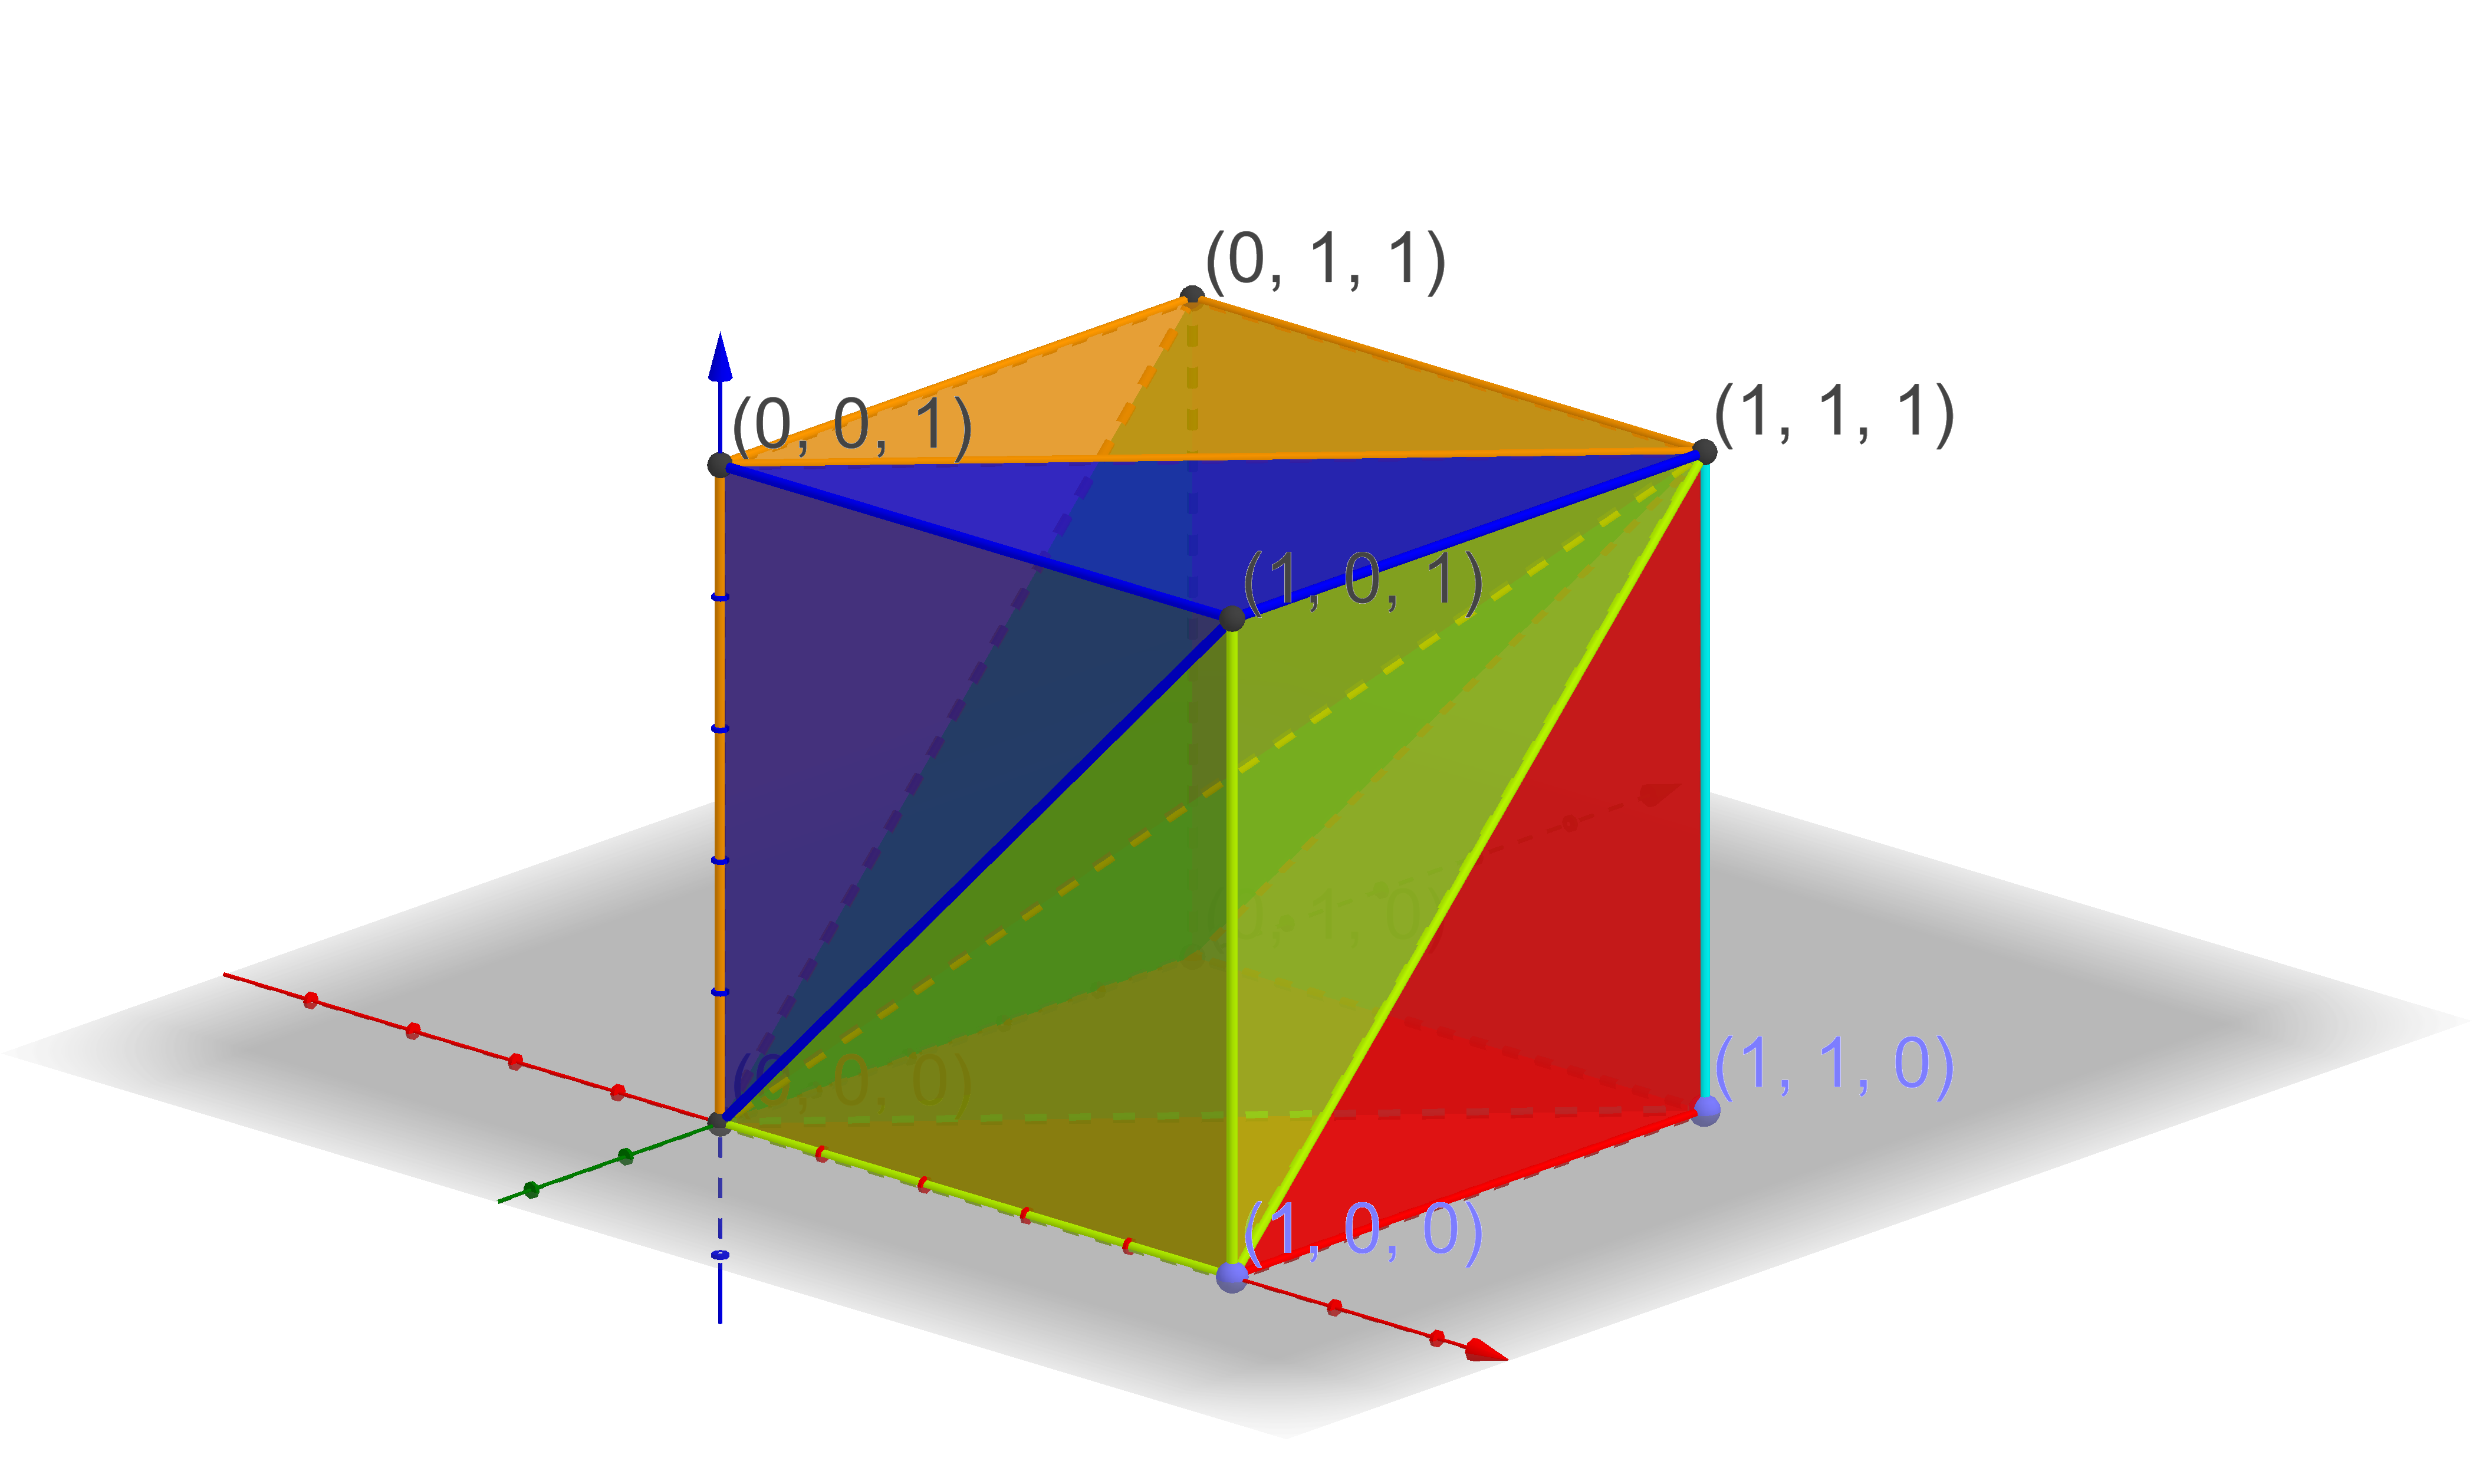
\includegraphics[scale=0.3]{img/triangulacioncubo.png}
\caption{Triangulación del $3$-cubo estándar de $\R^3$.}
\label{triangulacioncubo}
\end{figure}

Para aliviar la notación en las demostraciones que vienen a continuación, consideraremos $\Gamma$ el $m$-cubo estándar de $\R^m$, esto es, con raíz en el origen, direcciones $\{1,\dots,m\}$ y $\varepsilon=1$. Denotaremos los símplices de la triangulación de $\Gamma$ sencillamente como $\Delta_\sigma$ para $\sigma \in S_m$. Además, escribiremos $\bm{0}=(0,\dots,0)\in \R^m$ y $\bm{1}=(1,\dots,1)=e_1+\dots+e_m\in\R^m$.

\begin{proposicion}
Sea $x=(x_1,\dots,x_m)\in\Gamma$. Se tiene $x\in \Delta_\sigma$ si y solamente si $\sigma$ es una permutación que ordena las coordenadas de $x$ de mayor a menor, i.e., si $x_{\sigma(1)}\geq x_{\sigma(2)} \geq \dots \geq x_{\sigma(m)}$.
\end{proposicion}

\begin{proof}
Basta con ver como se escriben los puntos de $\Delta_\sigma$ en la base canónica de $\R^m$:
\begin{equation*}
\begin{gathered}
\lambda_0 \sigma_0 + \lambda_1 \sigma_1 + \dots + \lambda_m \sigma_m, \, \lambda_i \geq 0 , \, \sum_{i=0}^m \lambda_i = 1 \\
\Downarrow \\
\lambda_0 \bm{0} + \lambda_1 e_{\sigma(1)} + \dots + \lambda_m (e_{\sigma(1)}+\cdots+e_{\sigma(m)}), \, \lambda_i \geq 0 , \, \sum_{i=0}^m \lambda_i = 1 \\
\Downarrow \\
\lambda_1 e_{\sigma(1)} + \dots + \lambda_m (e_{\sigma(1)}+\cdots+e_{\sigma(m)}), \, \lambda_i \geq 0 , \, \sum_{i=1}^m \lambda_i \leq 1  \\ 
\Downarrow \\
(\lambda_1 + \dots \lambda_m) e_{\sigma(1)} +  \dots + \lambda_m e_{\sigma(m)}, \, \lambda_i \geq 0 , \, \sum_{i=1}^m \lambda_i \leq 1 
\end{gathered}
\end{equation*}

Si tomamos ahora ciertos $\mu_i$ definidos de tal forma que $\mu_{\sigma(i)} = \lambda_i + \dots + \lambda_m$, se tiene los puntos de $\Delta_\sigma$ escritos de la forma:

\begin{equation*}
\begin{gathered}
\mu_{\sigma(1)} e_{\sigma(1)} + \dots + \mu_{\sigma(m)} e_{\sigma(m)}, \, 1 \geq \mu_{\sigma(1)} \geq \dots \geq \mu_{\sigma(m)} \geq 0 \\
\Downarrow \\
\mu_1 e_1 + \dots + \mu_m e_m, \, 1 \geq \mu_{\sigma(1)} \geq \dots \geq \mu_{\sigma(m)} \geq 0
\end{gathered}
\end{equation*}

Dado que $x\in \Gamma$ se escribe como $ x = x_1 e_1+\dots+x_m e_m , \, 0 \leq x_i \leq 1 $, se tendrá $x \in \Delta_\sigma$ si y solamente si $x_{\sigma(1)}\geq x_{\sigma(2)} \geq \dots \geq x_{\sigma(m)}$, tal como queríamos demostrar.
\end{proof}

\begin{observacion}
La proposición anterior nos da la inclusión $\Gamma \subset \cup_{\sigma\in S_m} \Delta_\sigma $ ya que para todo punto existirá alguna permutación que ordene sus coordenadas.
\end{observacion}

\begin{observacion}
\label{obs_intersecciones}
Si $\sigma$ y $\tau$ son dos permutaciones distintas, la intersección $\Delta_\sigma \cap \Delta_\tau$ será el conjunto de puntos las coordenadas de los cuales pueden ordenarse de mayor a menor mediante $\sigma$ y también mediante $\tau$. En particular, éstos puntos de la intersección tendrán coordenadas iguales allí donde $\sigma$ y $\tau$ difieren. En la notación de la demostración anterior, la igualdad $\mu_{\sigma(i)} = \mu_{\sigma(j)}$ para $i < j$ implica $\lambda_i + \dots + \lambda_j + \dots + \lambda_m = \lambda_j + \dots + \lambda_m $ y por tanto $\lambda_i=\dots=\lambda_{j-i}=0$. Así, los puntos de la intersección de dos símplex de esta forma se definen por tener ciertas $\lambda_i=0$, y por tanto se escriben como combinación afín de sólo un subconjunto de los puntos iniciales. Con esto se tiene que la intersección de dos símplices es cara de ambos.
\end{observacion}

\begin{observacion}
Las caras $(m-1)$-dimensionales de un símplex $\Delta_\sigma$ son aquellas formadas por todos los puntos que forman $\Delta_\sigma$ salvo uno. En la notación de la proposición anterior, esto implica un único $\lambda_i=0$.
\begin{itemize}
\item Si se trata de $\lambda_0=0$ ---extraemos $\sigma_0$---, implica que alguna de las coordenadas sea 1 ($\mu_{\sigma(1)} = \sum_{i=1}^m \lambda_i =1$), mientras que si se trata de $\lambda_m=0$ ---extraemos $\sigma_m$---, la implicación es que alguna se las coordenadas sea 0 ($\mu_{\sigma(m)}=0$). El resto de coordenadas tienen que ser distintas\footnote{Decimos distintas en general: puede haber puntos que tengan coordenadas iguales, pero no existirán coordenadas que sean iguales para todos los puntos de la cara.} entre ellas porque si no existiría algún otro $\lambda_i'=0$. Así pues, en estos casos $\sigma$ es la única permutación que ordena las coordenadas de ésta cara.
\item Si se tiene $\lambda_i=0$ con $i \neq 0,m$, la implicación es que dos coordenadas sean iguales ($\mu_{\sigma(i)} = \mu_{\sigma(i-1)}$).
\end{itemize}
Se tiene así que para toda cara de un símplex $\Delta_\sigma$ existirá un único $\sigma'\neq\sigma$ tal que $\Delta_{\sigma'}$ contenga la misma cara si y solamente si se trata de una cara que no esté formada por $\bm{0}$ ni por $\bm{1}$. En tal caso, la permutación $\sigma'$ es el producto de $\sigma$ por una trasposición: la que permuta $\sigma(i)$ con $\sigma(i-1)$.   
\label{obs_carassimplice}
\end{observacion}

\begin{definicion}
Dado un complejo cúbico simplicial $K$, denotamos por $K^T$ el \emph{complejo simplicial asociado} a $K$ que se define maximalmente \footnote{Esto es, si $\Delta$ pertenece al conjunto, las caras de $\Delta$ también.} por todos los símplices $\Delta_\sigma(\Gamma)$ con $\Gamma \in K$ y $\sigma \in S_D$.
\end{definicion}

Nótese que $K^T$ es un complejo simplicial ya que las caras de cada simplex pertenecen al complejo por definición y la intersección de dos símplices será o bien nula o bien una cara de ambos por la Observación \ref{obs_intersecciones}.

\begin{proposicion}
Los complejos $K$ y $K^T$ tienen la misma realización geométrica.
\end{proposicion}

\begin{proof}
Se deduce de los resultados anteriores. De una parte, todo $\Delta_\sigma (\Gamma)$ está contenido en $\Gamma$, y por otro lado $\Gamma$ está contenido en $\bigcup_{\sigma} \Delta_\sigma (\Gamma)$. En particular, se tiene $\Gamma = \bigcup_{\sigma} \Delta_\sigma (\Gamma)$ y por tanto $\bigcup_{\Gamma \in K} \Gamma = \bigcup_{\Delta \in K^T} \Delta $.
\end{proof}

\subsubsection{Morfismo de triangulación}

Ahora ya tenemos definido para nuestro complejo cúbico $K$ un complejo simplicial $K^T$ que, como sabemos por el teorema de comparación \cite{Navarro}, tiene la homología del subespacio dado por su realización geométrica. Veremos ahora que con esta triangulación de $K$ podemos construir un morfismo de $R$-módulos entre el complejo de cadenas cúbicas de $K$ y el complejo de cadenas simpliciales de $K^T$.

\begin{definicion}
Sea $K$ un complejo cúbico y $K^T$ su complejo simplicial asociado. Se definen los \emph{morfismos $T_p$ de triangulación} de cadenas cúbicas $p$-dimensionales de $K$ a cadenas simpliciales $p$-dimensionales de $K^T$:
\Map{T_p}{Q_p(K)}{C_p(K^T)}{\Gamma=\Gamma_{P,D}}{\sum_{\sigma \in S_p} \epsilon(\sigma) \Delta_\sigma(\Gamma)}
donde $\epsilon(\sigma)$ indica el \emph{signo} de la permutación $\sigma$.
\end{definicion}

\begin{proposicion}
Los morfismos $T_p$ forman un morfismo de complejos de $R$-módulos entre $Q_*(K)$ y $C_*(K^T)$. Esto es, el diagrama
\begin{equation*}
\xymatrix{
\cdots \ar[r]    & Q_{p+1}(K) \ar[d]_{T_{p+1}}\ar[r]^{\partial_{p+1}}   & Q_{p}(K) \ar[d]_{T_{p}}\ar[r]^{\partial_{p}}    & Q_{p-1}(K) \ar[d]_{T_{p-1}}\ar[r] & \cdots \\
\cdots \ar[r]    & C_{p+1}(K^T) \ar[r]^{\partial'_{p+1}}                & C_{p}(K^T) \ar[r]^{\partial'_{p}}               & C_{p-1}(K^T) \ar[r]               & \cdots
}
\end{equation*}
conmuta para toda $p \geq 0$. Denotamos por $T_*$ dicho morfismo de complejos.
\end{proposicion}

\begin{proof}
Demostraremos que diferencial y triangulación conmutan para el $m$-cubo estándar $\Gamma$ de $\R^m$. El razonamiento se extiende de forma natural para todo $p$-cubo de un complejo $K$, y por linealidad para todo elemento de $Q_p(K)$.

De una parte, desarrollaremos $T_{m-1} \circ \partial_m (\Gamma) = T_{m-1} \left( \partial_m (\Gamma) \right)$. En las siguientes líneas, denotamos $\hat{k}=\{1,\dots,m\}\backslash\{k\}$.
\begin{align*}
T_{m-1} \left( \partial_m (\Gamma) \right) &= T_{m-1} \left( \sum_{k=1}^m (-1)^{k} \Gamma_{\bm{0},\hat{k}} - \sum_{k=1}^m (-1)^{k} \Gamma_{e_k,\hat{k}} \right) \\
                                           &= \sum_{k=1}^m (-1)^{k} T_{m-1} \left( \Gamma_{\bm{0},\hat{k}} \right) - \sum_{k=1}^m (-1)^{k} T_{m-1} \left( \Gamma_{e_k,\hat{k}} \right) \\
                                           &= \sum_{\substack{k=1,\dots,m \\ \sigma \in S_{m-1}}} (-1)^{k} \epsilon(\sigma) \Delta_\sigma\left( \Gamma_{\bm{0},\hat{k}} \right) - \sum_{\substack{k=1,\dots,m \\ \sigma \in S_{m-1}}} (-1)^{k} \epsilon(\sigma) \Delta_\sigma \left( \Gamma_{e_k,\hat{k}} \right) 
\end{align*}
El resultado es una suma alternada de los símplices que tienen como puntos todos los caminos para ir desde $\bm{0}$ a $\bm{1}-e_k$ y todos los caminos desde $e_k$ hasta $\bm{1}$, para cada $k=1,\dots,m$. Los términos de esta suma no se repiten, ya que son triangulaciones de cubos diferentes. Abreviaremos $\Delta_{\sigma,k}^{\bm{0}}= \Delta_\sigma ( \Gamma_{\bm{0},\hat{k}})$ y $\Delta_{\sigma,k}^{\bm{1}}= \Delta_\sigma ( \Gamma_{e_k,\hat{k}})$. De esta forma, se tiene:
$$
T_{m-1} \left( \partial_m (\Gamma) \right) = \sum_{\substack{k=1,\dots,m \\ \sigma \in S_{m-1}}} (-1)^{k} \epsilon(\sigma) \Delta_{\sigma,k}^{\bm{0}} - (-1)^{k} \epsilon(\sigma) \Delta_{\sigma,k}^{\bm{1}}
$$

Miremos ahora como se desarrolla $\partial_m \circ T_m (\Gamma) = \partial_m \left( T_m (\Gamma) \right)$.
\begin{align*}
\partial'_m \left( T_m (\Gamma) \right) &= \partial'_m \left( \sum_{\tau \in S_m} \epsilon(\tau) \Delta_\tau(\Gamma) \right) \\
                                        &= \sum_{\tau \in S_m} \epsilon(\tau) \partial'_m \left(  \Delta_\tau(\Gamma) \right) \\
                                        &= \sum_{\tau \in S_m} \epsilon(\tau) \partial'_m \left(  [\tau_0,\dots,\tau_m] \right) \\
                                        &= \sum_{\substack{l=0,\dots,m \\ \tau \in S_m}} \epsilon(\tau) (-1)^l [\tau_0,\dots,\hat{\tau_k},\dots,\tau_m]
\end{align*}
Lo que se obtiene es una suma alternada de símplices formados por todos los caminos de $\bm{0}$ a $\bm{1}$, cada uno de ellos repetido $m+1$ veces quitándole cada uno de sus puntos $\tau_k$.

En este desarrollo de $\partial'_m \left( T_m (\Gamma) \right)$ sí hay términos repetidos. Como veíamos en la Observación \ref{obs_carassimplice}, la cara $[\tau_0,\dots,\hat{\tau_l},\dots,\tau_m]$ de $\Delta_\tau$ será también cara de un (único) $\Delta_\tau'$ si y sólo si la coordenada que extraemos $\tau_l$ no es la primera ni la última ($l \neq 0,m$). En tal caso, como veíamos en la Observación \ref{obs_carassimplice}, $\tau$ y $\tau'$ difieren en una permutación de forma que tienen signo contrario y los dos términos $[\tau_0,\dots,\hat{\tau_l},\dots,\tau_m]$ y $[\tau'_0,\dots,\hat{\tau'_l},\dots,\tau'_m]$ se cancelarán en la suma\footnote{Nótese que en ambos casos $\tau$ y $\tau'$, la posición $l$ que se extrae es la misma ya que existe un orden natural de los puntos de cada símplex dado por \emph{el número de aumentos} que se han dado hasta ese punto. Los símplices $\tau$ y $\tau'$ tienen todos los puntos iguales salvo uno, por ello en el que difieren no puede corresponder a un número distinto de aumentos en cada símplice.}.

Los términos que se mantienen son aquellos en los que quitamos el $\bm{0}$ y el $\bm{1}$, que escribiremos respectivamente $\Delta_\tau^{\bm{0}}$ y $\Delta_\tau^{\bm{1}}$, teniéndose así:
$$
\partial'_m \left( T_m (\Gamma) \right) = \sum_{\tau \in S_m} \epsilon(\tau) \Delta_\tau^{\bm{0}} + \epsilon(\tau) (-1)^m \Delta_\tau^{\bm{1}}
$$

Estos símplices se corresponden justamente con los que se tienen en el desarrollo de $T_{m-1} \left( \partial_m (\Gamma) \right)$. Ahora sólo es necesario ver que figuran en ambos sitios con el mismo signo.

Para ello sólo hace falta notar que para cada $k=1,\dots,m$ y cada $\sigma \in S_{m-1}$, la permutación $\tau \in S_m$ tal que $\Delta_\tau^{\bm{0}}$ corresponda con $\Delta_{\sigma,k}^{\bm{1}}$ es aquélla que manda $k$ al 1, y los elementos $\sigma(i)$ a $\sigma(i)+1$, si $i<k$ y al mismo $\sigma(i)$ cuando $i > k$. En otras palabras, considerando $\sigma \in S_{m-1} \subset S_m$, la permutación $\tau$ se escribe como el siguiente producto de $S_m$:
$$ \tau = (1,2,\dots,k) \circ \sigma $$
donde $(1,2,\dots,k) \in S_m$ es un ciclo de orden $k$. Con esto podemos ver que dicha $\tau$ cumple $\epsilon(\tau)=(-1)^{k-1}\epsilon(\sigma)$.

De forma completamente análoga, la permutación $\tau'$ cuyo símplex $\Delta_\tau^{\bm{1}}$ corresponde con $\Delta_{\sigma,k}^{\bm{0}}$ es aquélla que aplica $\sigma$ y luego envía $k$ a $m$ y resta uno a los que son mayores que $k$: 
$$ \tau' = (m,m-1,\dots,k) \circ \sigma $$
de donde se tiene $\epsilon(\tau) = (-1)^{m-k} \epsilon(\sigma)$. 

Si ahora escribimos la suma $\partial'_m ( T_m (\Gamma) )$ indexada sobre $k=1,\dots,m$ y $\sigma \in S_{m-1}$ usando esta relación, se obtiene:
\begin{align*}
\partial'_m \left( T_m (\Gamma) \right) &= \sum_{\tau \in S_m} \epsilon(\tau) \Delta_\tau^{\bm{0}} + \epsilon(\tau) (-1)^m \Delta_\tau^{\bm{1}} \\
                                        &= \sum_{\substack{k=1,\dots,m \\ \sigma \in S_{m-1}}} (-1)^{k-1} \epsilon(\sigma) \Delta_{\sigma,k}^{\bm{1}} + (-1)^m(-1)^{m-k} \epsilon(\sigma) \Delta_{\sigma,k}^{\bm{0}} \\
                                        &= \sum_{\substack{k=1,\dots,m \\ \sigma \in S_{m-1}}} (-1)^{k} \epsilon(\sigma) \Delta_{\sigma,k}^{\bm{0}} - (-1)^k \epsilon(\sigma) \Delta_{\sigma,k}^{\bm{1}} \\
                                        &= T_{m-1} \left( \partial_m (\Gamma) \right)
\end{align*}
\end{proof}

\subsubsection{Teorema de comparación de la homología cúbica}

Dedicamos este apartado exclusivamente a demostrar que la homología cúbica de un complejo cúbico $K$ (tal como aquí la hemos definido) es equivalente a la homología del subespacio de $\R^n$ que ocupa, esto es, la homología singular de su realización geométrica $\geom{K}$ como espacio topológico. En particular, esto nos dirá que dos complejos cúbicos con realizaciones geométricas homótopas tienen los mismos grupos de homología.

\begin{lema}
Sea $s$ el complejo cúbico formado por un único cubo $\Gamma$. Entonces $s$ es contráctil, i.e., $H_p(s)=0$ para toda $p>0$.
\label{lema}
\end{lema}

\begin{proof}
Para simplificar la notación, consideraremos $\Gamma$ el $m$-cubo estándar de $\R^m$. Haremos inducción sobre la dimensión $m$ de $\Gamma$. Si $m=0$ entonces es evidente que los grupos de homología $H_p(s)$ serán 0 para $p > 0$ ya que $s$ no contiene ninguna cara de dimensión $p > 0$. Supongamos ahora que $\Gamma$ es el cubo de dimensión $m>0$ y supondremos cierto el resultado para cualquier complejo cúbico formado por un único cubo de dimensión más pequeña que $m$.

Lo demostraremos por reducción al absurdo. Supóngase que para algún $p \leq m$ se tiene $H_p(s) \neq 0$. Dicho de otra forma, tenemos algún $C \in Q_p(s)$ tal que $\partial_p(C) \neq 0$ y $C \notin \Img{\partial_{p+1}}$. Escribimos $C$ como la suma formal de $p$-cubos $C=a_1 c_1+\dots+a_r c_r$ donde los coeficientes $a_i \neq 0$ pertenecen al anillo $R$ sobre el que se defina el complejo de cadenas, y los $c_i=\Gamma_{P_i,D_i}$ son $p$-cubos pertenecientes al complejo $s$. 

Supongamos que existe algún $c_i=\Gamma_{P_i,D_i}$ tal que la primera coordenada del punto raíz es $P_1 = 1$ ---nótese que esto conlleva que $1 \notin D_i$ y todos los puntos de $c_i$ tienen primera coordenada 1---. En tal caso, $c_i$ es una cara del $(p+1)$-cubo que tiene como raíz el mismo punto $P_i$ pero con primera coordenada igual a 0, y las direcciones $D_i$ añadiéndole la primera, i.e., el cubo $q_i=\Gamma_{P_i-e_1,\{1\} \cup D_i}$. Nótese que, en particular, $c_i$ aparece con signo positivo en la diferencial de $q_i$ ya que corresponde al primer término del segundo sumatorio. El resto de términos tienen primera coordenada 0, ya que parten de $P_i-e_1$ o bien de $P_i-e_1+e_k$ con algún $e_k \neq e_i$. Siendo de esta forma podemos considerar $C' = C - a_i \partial_{p+1} (q_i)$ que será una cadena de cubos donde ya no aparece $c_1$ ---que se cancela--- y en la cual no se ha añadido ningún cubo cuya raíz tenga primera coordenada 1. Nótese que dicho $C'$ es un elemento del núcleo de la diferencial ya que $\partial_p(C') = \partial(C) - a_i \partial_p\partial_{p+1}(q_i)=0+0=0$. Razonando inductivamente de esta forma podríamos quitar todos los cubos cuya raíz tenga primera coordenada igual a 1 y seguir teniendo un elemento del núcleo de la diferencial.

Supongamos entonces que en nuestra cadena $C$ todo cubo $c_i$ tiene raíz con primera coordenada 0. Si no existe ningún $c_i$ que tenga la dirección 1, i.e., tal que $1 \in D_i$, entonces la cadena $C$ está contenida en el $(m-1$)-cubo $\Gamma_{\bm{0},\hat{D}_1}$ y entonces por hipótesis de inducción entraríamos en contradicción. Sea $c_i$ un cubo tal que $1 \in D_i$. En su diferencial, aparecerá el término $\Gamma_{P_i+e_1,D_i \backslash \{ 1\}}$, el cual sólo puede ser cara de $c_i=\Gamma_{P_i,D_i}$ o de $\Gamma_{P_i+e_1,D_i}$. Como todos los cubos de $C$ tienen raíz con primera coordenada 1, el cubo $\Gamma_{P_i+e_1,D_i}$ no se corresponde a ningún $c_j$ de la cadena $C$. Se tiene entonces que en el desarrollo de la diferencial de $C$
$$ \partial_p(C) = a_1\partial_p(c_1) + \dots + a_i\partial_p(c_i) + \cdots + a_r \partial_p(c_r) $$
aparece el término $a_i \Gamma_{P_i+e_1,D_i \backslash \{ 1\}}$ que no se cancela con ningún otro término de la suma, contradiciendo que $\partial_p (C) = 0$.

Se concluye por tanto que no puede existir dicho $C$ y por tanto los grupos de homología son triviales para todo $p>0$.
\end{proof}

\newpage
\begin{teorema}
Sea $K$ un complejo cúbico y $K^T$ su complejo simplicial asociado. El morfismo de triangulación $T_p$ induce un isomorfismo entre los grupos de homología $H_p(K)$ y $H_p(K^T)$.
\end{teorema}

\begin{proof}
Haremos una primera inducción sobre la dimensión del complejo $K$. Si el complejo $K$ es de dimensión 0 (sólo puntos aislados) entonces ya el propio $T_p$ es una biyección entre $Q_p(K)$ y $C_p(K^T)$, ya que $K$ y $K^T$ tienen los mismos vértices y no habría nada en dimensiones superiores.

Sea ahora $K$ un complejo cúbico de dimensión $i>0$ y supondremos el resultado cierto para cualquier complejo de dimensión $i-1$. Haremos una segunda inducción sobre el número de cubos de dimensión $i$ del complejo $K$. Si $K$ no tiene ningún $i$-cubo entonces la dimensión de $K$ es inferior a $i$ y el resultado se tiene por la primera inducción. Supongamos ahora que $K$ se construye añadiendo un $i$-cubo a un subcomplejo $L$ sobre el que supondremos cierto el resultado. Así, denotamos $K=L\cup\{\Gamma\}$ con $\Gamma$ un $i$-cubo.

La inclusión $L\subset K$ nos permite escribir una sucesión exacta corta de complejos de $R$-módulos, tomando el dual de dicha inclusión, tal como sigue.
\begin{equation*}
\xymatrix{
0 \ar[r]    & Q_*(L) \ar[r]^{\iota}   & Q_*(K) \ar[r]    & \quotient{Q_*(K)}{Q_*(L)} \ar[r] & 0
}
\end{equation*}
De forma completamente análoga podemos construir una sucesión exacta corta con los complejos de cadenas simpliciales a partir de la inclusión $L^T \subset K^T$. 
\begin{equation*}
\xymatrix{
0 \ar[r]    & C_*(L^T) \ar[r]^{\iota}   & C_*(K^T) \ar[r]    & \quotient{C_*(K^T)}{C_*(L^T)} \ar[r] & 0
}
\end{equation*}

Ambas sucesiones las podemos juntar en un diagrama usando los morfismos de triangulación de $L$ (que denotamos $T_*^L$), el de $K$ (que denotamos $T_*$) y el que induce la triangulación de $K$ sobre los complejos cocientes de la derecha (que llamaremos sencillamente $f_*$).
\begin{equation*}
\xymatrix{
0 \ar[r] & Q_*(L) \ar[r]^{\iota}\ar[d]_{T_*^L} & Q_*(K) \ar[r]\ar[d]_{T_*} & \quotient{Q_*(K)}{Q_*(L)} \ar[r] \ar[d]_{f_*} & 0 \\
0 \ar[r]    & C_*(L^T) \ar[r]^{\iota}   & C_*(K^T) \ar[r]    & \quotient{C_*(K^T)}{C_*(L^T)} \ar[r] & 0
}
\end{equation*}

Dichos morfismos inducen un diagrama entre los grupos de homología de la sucesión exacta larga de la forma
\begin{equation*}
\xymatrix@C=0.8em{
\cdots \ar[r]  & H_{p+1}(K,L) \ar[r]\ar[d]_{\tilde{f}_{p+1}} & H_p(L) \ar[r]\ar[d]_{\tilde{T}_p^L} & H_p(K) \ar[r]\ar[d]_{\tilde{T}_p} & H_p(K,L) \ar[r] \ar[d]_{\tilde{f}_p} & H_{p-1}(L)\ar[d]_{T_{p-1}^{L}}\ar[r]  & \cdots \\
\cdots \ar[r]  & H_{p+1}(K^T,L^T) \ar[r]    & H_p(L^T) \ar[r]   & H_p(K^T) \ar[r]    & H_p(K^T,L^T) \ar[r] & H_{p-1}(L^T)\ar[r]  &\cdots
}
\end{equation*}
donde $\tilde{T}_p^L$ y $\tilde{T}_{p-1}^L$ son isomorfismos por inducción. Por tanto si $\tilde{f}_p$ y $\tilde{f}_{p-1}$ son también isomorfismos entonces, por el Lema de los Cinco \cite{Navarro}, también lo será $\tilde{T}_p$ y habremos terminado. La demostración se reduce entonces a ver que la triangulación induce un isomorfismo entre los grupos de homología del par $(K,L)$ y del par $(K^T,L^T)$.

Sea $s$ el complejo cúbico generado por el cubo $\Gamma$ en el cual difieren $K$ y $L$, y $\partial s$ el complejo cúbico generado por las caras de $\Gamma$. Comenzaremos por ver que la triangulación induce un isomorfismo entre los grupos de homología del par $(s, \partial s)$ y el par $(s^T, \partial s^T)$. Con una construcción muy similar a la anterior, los morfismos de triangulación de $s$ y $\partial s$ generan morfismos entre los grupos de homología de la sucesión exacta larga, que escribimos a continuación centrada en $H_p(s, \partial s)$.
\begin{equation*}
\xymatrix@C=0.8em{
\cdots \ar[r]  & H_{p}(\partial s) \ar[r]\ar[d]_{\tilde{T}_{p}^{\partial s}} & H_p(s) \ar[r]\ar[d]_{\tilde{T}_p^s} & H_p(s,\partial s) \ar[r]\ar[d]_{\tilde{f'}_p} & H_{p-1}(\partial s) \ar[r] \ar[d]_{\tilde{T}_{p-1}^{s}} & H_{p-1}(s)\ar[d]_{T_{p-1}^s}\ar[r]  & \cdots \\
\cdots \ar[r]  & H_{p}(\partial s^T) \ar[r] & H_p(s^T) \ar[r] & H_p(s^T,\partial s^T) \ar[r] & H_{p-1}(\partial s^T) \ar[r] & H_{p-1}(s^T) \ar[r]  & \cdots 
}
\end{equation*}
Al ser $\partial s$ un complejo cúbico de dimensión $i-1$, se tiene por hipótesis de inducción que la triangulación de éste induce un isomorfismo en los grupos de homología, con lo cual $\tilde{T}_p^{\partial s}$ y $\tilde{T}_{p-1}^{\partial s}$ son isomorfismos. Por otro lado, los grupos de homología $H_p(s)$ y $H_p(s^T)$ son nulos para todo $p>0$ \footnote{En el caso de $H_p(s)$ ---homología cúbica--- lo hemos visto en el Lema \ref{lema}, mientras que en el caso de $H_p(s^T)$ ---homología simplicial--- es por el hecho de que se trata de la triangulación de un cubo (contráctil).}\footnote{En $p=0$ no son nulos de hecho, pero en cualquier caso la triangulación es un isomorfismo en dimensión 0 ya que la correspondencia de puntos es biyectiva.}, con lo cual los morfismos $\tilde{T}_p^s$ y $\tilde{T}_{p-1}^s$ son también isomorfismos ---son el morfismo trivial, de hecho---. Se concluye por el Lema de los Cinco que $\tilde{f'}_p$ es tambíen un isomorfismo.

Para expandir este resultado ahora sobre los pares $(K,L)$ y $(K^T, L^T)$ haremos un paso por la homología singular para hacer uso del Teorema de Escisión, para luego volver a homología simplicial a partir del Teorema de Comparación (pueden consultarse ambos teoremas en \cite{Navarro}). El diagrama con el que trabajaremos es el siguiente:
\begin{equation*}
\xymatrix{
                         &                               & H_p(K,L) \ar[r]^{\tilde{f}_p}        & H_p(K^T,L^T) \\
H_p(s,\partial s) \ar[r]^{h_1} \ar@/^1.0pc/@{^{(}->}[rru] & H_p(s^T,\partial s ^T) \ar[r]^{h_2} & H_p(\geom{s},\geom{\partial s}) \ar@{^{(}->}[r]^{h_3} & H_p(\geom{K},\geom{L}) \ar[u]^{h_4}  
}
\end{equation*}
Véase que la inclusión del par $(s, \partial s)$ en $(K,L)$ es un isomorfismo por construcción: ambos pares difieren únicamente en un cubo $\Gamma$, con lo cual la inclusión a nivel de cadenas de cubos es una mera biyección que envía $\Gamma$ a $\Gamma$ en dimensión $i$, y es 0 para el resto de dimensiones. De esta manera, si demostramos que son isomorfismos los $h_1$, $h_2$, $h_3$ y $h_4$ del camino de abajo, se tendrá que $\tilde{f}_p$ es un isomorfismo tal como queremos demostrar.

El morfismo $h_1$ es el caso particular del cubo que hemos visto antes, mientras que $h_2$ y $h_4$ son isomorfimos por el Teorema de Comparación y el hecho que la realización geométrica de la triangulación de un complejo cúbico coincide con la realización geométrica del propio complejo cúbico.

Falta ver $h_3$ y para ello usamos el Teorema de Escisión sobre el par $(\geom{K}, \geom{L})$ respecto al subespacio $U=\geom{K}\backslash\geom{s}$. Nótese que definido de esta forma se tiene $\geom{K} \backslash U = \geom{s}$ y $\geom{L} \backslash U = \geom{\partial s}$. Sea $B= \geom{K} \backslash \{ b \}$ donde $b$ es el baricentro de $\Gamma$. Entonces $\geom{L}$ y $\geom{L} \backslash U$ son retractos de deformación de $B$ y $B \backslash U$, respectivamente. Como $\bar{U} \subset \mathring{B}=B$ y $U \subset L \subset B \subset X$, entonces $U$ es escisivo en $(K,L)$ (véase \cite{Navarro}) y se tiene por el Teorema de Escisión un isomorfismo
$$ H_p(\geom{s}, \geom{\partial s}) = H_p(\geom{K} \backslash U, \geom{L} \backslash U) \cong H_p(\geom{K}, \geom{L}) $$
dado por la inclusión natural, que se corresponde con nuestro $h_3$.

\end{proof}

\begin{corolario}
La homología cúbica de un complejo cúbico $K$ es equivalente a la homología singular de su realización geométrica $\lvert K \rvert$ como espacio topológico. En particular, estos grupos de homología son invariantes por homotopía.
\end{corolario}

\begin{proof}
Es consecuencia inmediata del teorema anterior, el teorema de comparación entre homología simplicial y singular, y el hecho que $\lvert K^T \rvert = \lvert K \rvert$. 
\end{proof}

\newpage
\NewPage
\cleardoublepage
\section{Filtraciones mediante KDE}

% --------------------------------
%
% SECCIÓN 4: FILTRACIONES MEDIANTE KDE
%
% --------------------------------

En esta sección se desarrolla el método para crear una filtración a partir de un estimador de densidad mediante kernels (\emph{Kernel Density Estimator, KDE}) de la nube de datos. Haremos primero una breve introducción de lo que es un KDE para luego definir formalmente la construcción del complejo cúbico y la filtración mediante dicho KDE.

\subsection{Estimadores kernel de densidad (KDE)}

Una práctica habitual en estadística es el uso de \emph{kernels} para estimar la función de densidad de una variable aleatoria dado un muestreo de ella. En general, si se tiene un conjunto $X= \{x_1,\dots,x_N \} \subset \R^n$ de variables aleatorias independientes idénticamente distribuidas que responden a una función de densidad $\map{f}{\R^n}{\R}$, el método de KDE consiste en estimar dicha densidad mediante
$$ \hat{f}_h(x) = \frac{1}{Nh} \sum_{i=0}^N K\left( \frac{x-x_i}{h}\right) $$
donde $K$ es el \emph{kernel} ---una función no negativa que integra 1--- y $h>0$ es un parámetro a fijar llamado \emph{ancho de banda} o \emph{bandwidth}.

Los ejemplos de kernel más ampliamente usados son el kernel uniforme, el triangular, el de Epanechnikov i el normal. La elección del kernel y el bandwidth a utilizar debe ir a cargo a de la persona responsable de analizar los datos, según la información que se tenga de ellos (veáse \cite{Scheid} y \cite{Chouaib}).

\begin{figure}[h!]
\centering
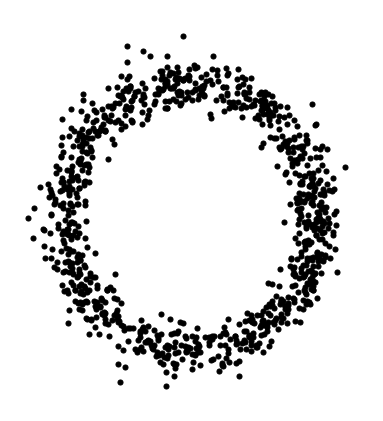
\includegraphics[scale=0.45]{img/cloudzoom.png}
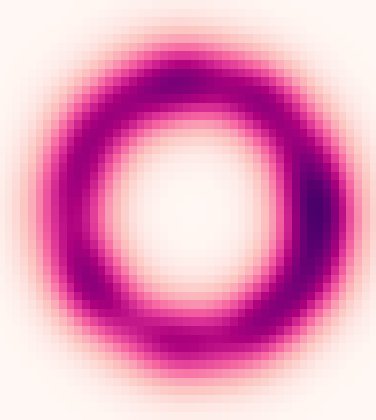
\includegraphics[scale=0.45]{img/kdezoom.png}
\caption{Ejemplo de nube de datos y su KDE gaussiano.}
\label{kde}
\end{figure}

Para los fines del método que se desarrolla en este trabajo, nos basta con el hecho de que el KDE, sea cual sea el kernel o el bandwidth empleado, nos da una función $\map{f}{\R^n}{\R}$ que toma valores más altos allí donde la concentración de puntos es mayor. Esto nos aporta un mecanismo para \emph{dar forma} de una manera coherente a la figura que subyace de la nube de datos.

La Figura \ref{kde} muestra un ejemplo visual de lo que es un KDE. Para la nube de datos de $\R^2$ que se muestra en la imagen de la izquierda, el KDE es una función $\map{f}{\R^2}{\R}$ que se representa con una gráfica de colores en la imagen de la derecha. El KDE toma valores más altos (color más intenso en la Figura \ref{kde}) allí donde la concentración de puntos es mayor.

Para más información sobre los KDE, redirigimos al lector a \cite{Scheid} y \cite{Chouaib} que analizan con profundidad las diferencias entre cada kernel y el ancho de banda utilizado, y cuáles son los criterios que se deben seguir para su elección.

\subsection{Filtraciones mediante KDE. Formalización}

Sea $S \subset \R^n $ una nube de $N$ puntos del espacio euclídeo, y sea $\map{f}{\R^n}{\R}$ un KDE para esta nube de datos.

El primer paso consiste en construir una cuadrícula $n$-dimensional de una precisión fijada $\varepsilon>0$ sobre el espacio que ocupa la nube de datos. Formalmente, para cada dimensión de $\R^n$ tomamos puntos equidistantes ---con distancia $\varepsilon$--- de la forma $x_1^{(i)},\dots,x_{n_i}^{(i)}\in \R$ tales que $x_1^{(i)}<\min_{x\in S}{\pi_i(x)}$ y $x_{n_i}^{(i)}>\max_{x\in S}{\pi_i(x)}$ para $i=1,\dots,n$ \footnote{Usamos $\map{\pi_i}{\R^n}{\R}$ para denotar la proyección de sobre el eje $i$ de la base canónica. Esto es, si $x\in\R^n$, $\pi_i(x)$ es la $i$-ésima coordenada de $x$ en la base canónica.}. El producto cartesiano de estos puntos nos dará los puntos de una cuadrícula en $\R^n$ que llamaremos $G$.
$$ G = \prod_{i=1}^n \{x_i\}_{i=1,\dots,n_i} \subset \R^n $$

\begin{figure}[h!]
\centering
%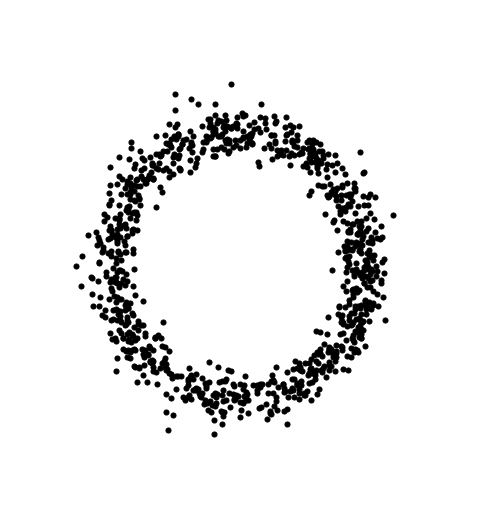
\includegraphics[scale=0.35]{img/cloud.png}
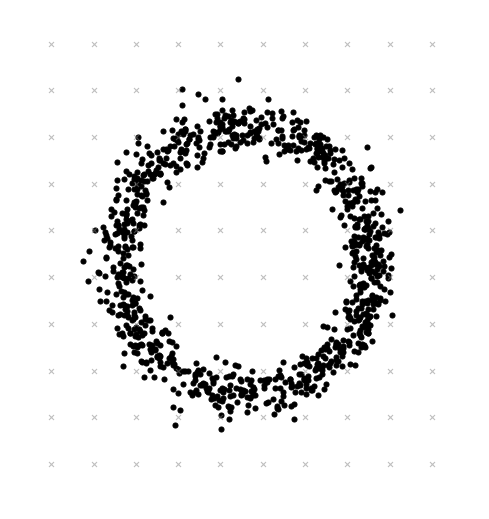
\includegraphics[scale=0.45]{img/grid.png}
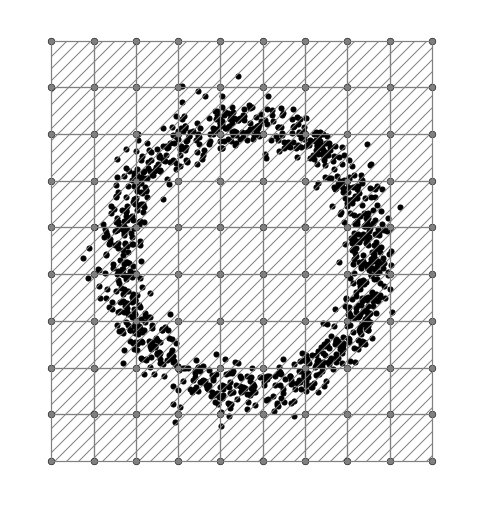
\includegraphics[scale=0.45]{img/complexandcloud.png}
\caption{Cuadrícula y complejo cúbico sobre $\R^2$.}
\label{grid}
\end{figure}

Sobre esta cuadrícula construimos cubos simpliciales como los que se definen en la Sección 2 para formar un complejo cúbico simplicial. Esencialmente, se toman todos los cubos con raíz en un punto de la cuadrícula y con direcciones cualquier subconjunto de $\N_n = \{1,\dots,n\}$, salvo aquellos que están \emph{al final}, i.e., no se toman cubos con dirección $d_i$ si la coordenada $d_i$ del punto raíz es la más alta en esa dimensión, ya que en tal caso tendría caras formadas por puntos de fuera de la cuadrícula. Formalmente escribiríamos 
$$ K = \lbrace \Gamma_{\varepsilon,P,D} \tq P\in G, \, D \in \mathcal{P}(\N_n), \, \pi_i(P) \neq x_{n_i}^{(i)}, \, \forall i \in D \rbrace $$

Definido de esta forma, el conjunto $K$ forma un complejo cúbico simplicial ya que toda cara de un elemento $K$ está contenida en $K$ y además la intersección de dos elementos es una cara de ambos.

La función KDE $\map{f}{\R^n}{\R}$ induce una aplicación sobre el complejo $K$
\Map{\tilde{f}}{K}{\R}{\Gamma}{\inf \lbrace f(x) \tq x \in \Pi(\Gamma) \rbrace}
que es no decreciente para secuencias crecientes de caras, i.e., si $\sigma$ es una cara de $\Gamma$ entonces $f(\sigma) \leq f(\Gamma)$ ya que $\Pi(\sigma) \subseteq \Pi(\Gamma)$. Tal como comentábamos en la Sección 2, esto define una filtración $\mathcal{F}_f = \{K_a\}_{a\in\R}$ sobre $K$ dada por $K_a = \tilde{f}^{-1}\left((-\infty,a]\right)$. Diremos que $\mathcal{F}$ es la filtración cúbica que se construye mediante $f$ sobre la cuadrícula $G$.

Para mayor comprensión, nótese que la filtración consiste en ir añadiendo de uno en uno\footnote{Si $f$ es inyectiva sobre $G$.} los puntos de la cuadrícula (que son los $0$-cubos de $K$) por orden según lo alto que sea su valor cuando se evalúan en $f$. Un $m$-cubo de $K$ con $m \geq 1$ se añade en el momento que todos sus puntos han sido añadidos. La Figura \ref{kde_filtration} muestra algunos elementos de la filtración para el KDE que se mostraba en la Figura \ref{kde}.

\begin{figure}[h!]
\centering
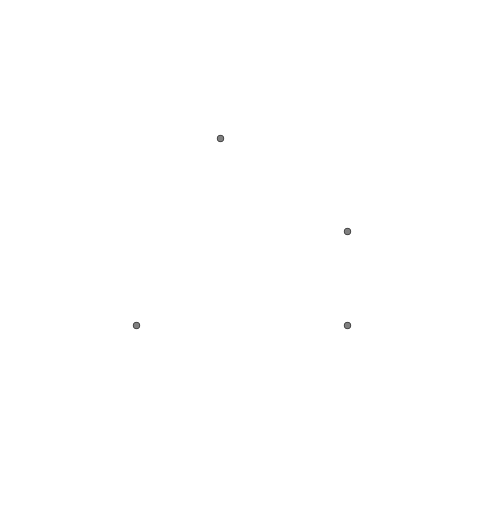
\includegraphics[scale=0.33]{img/f1.png}
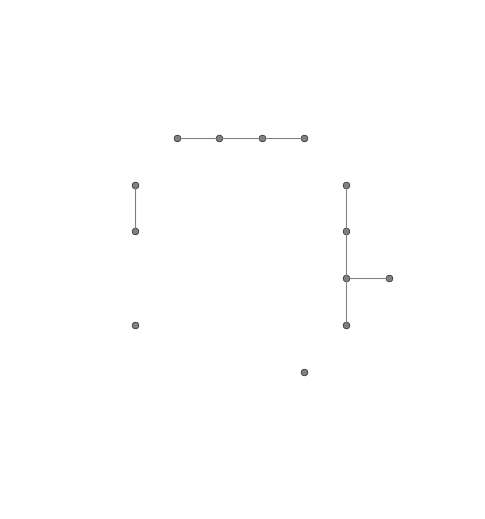
\includegraphics[scale=0.33]{img/f2.png}
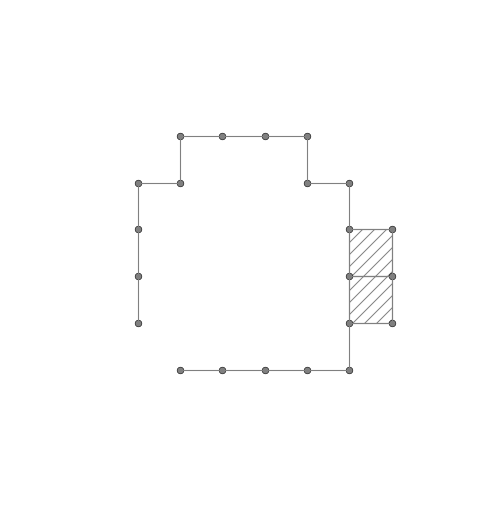
\includegraphics[scale=0.33]{img/f3.png}
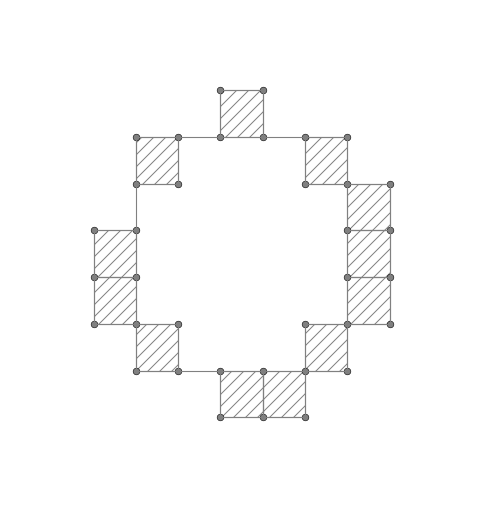
\includegraphics[scale=0.33]{img/f4.png}
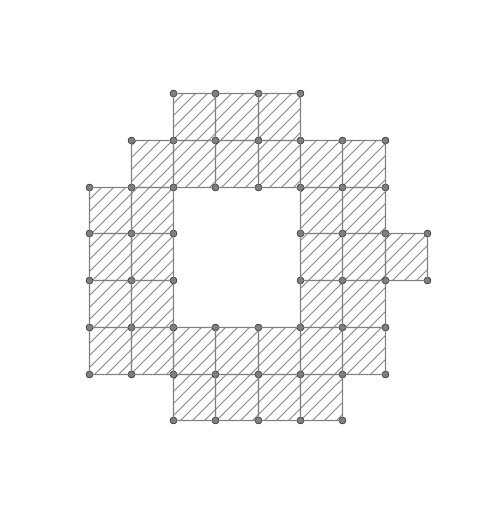
\includegraphics[scale=0.33]{img/f5.png}
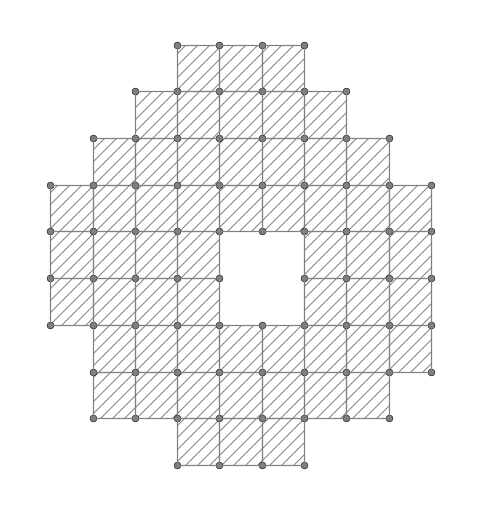
\includegraphics[scale=0.33]{img/f6.png}
\caption{Filtración mediante el KDE de la Figura \ref{kde}}
\label{kde_filtration}
\end{figure}

Cada elemento de la filtración $\mathcal{F}$ es un complejo cúbico simplicial sobre el que se puede calcular (con álgebra lineal, en un número finito de pasos dada la finitud del complejo) la homología cúbica definida en la Sección 3. Como hemos visto, esta homología coincide con la homología (singular) de $\lvert K \rvert$ como subespacio topológico de $\R^n$.

Como hemos descrito en la Sección 2, las inclusiones en la filtración nos permiten hablar de \emph{generadores de persistencia} para la filtración $\mathcal{F}$, que tienen definidos sus instantes de nacimiento y muerte y que pueden representarse en un diagrama de persistencia o en un código de barras que pueden ser analizados para estimar la forma subyacente de la nube de datos $S$.

\newpage
\section{Implementación}

% --------------------------------
%
% SECCIÓN 5: IMPLEMENTACIÓN
%
% --------------------------------

Se ha desarrollado un módulo de Python que implementa el método de filtraciones mediante KDE para una nube de datos $S \in \R^n$ de dimensión arbitraria. Una versión beta de éste software ya ha sido subida a los repositorios de PyPI con el nombre \texttt{Cubix}, con lo que para poder instalarlo en un Linux basta con tener instalado \texttt{pip} y ejecutar en la consola

\begin{lstlisting}[language=bash]
  $ pip install cubix 
\end{lstlisting}

El módulo contiene métodos para generar nubes de datos de algunas formas básicas ---como $S^1$, $S^1 \vee S^1$, $S^2$, $T^2$ y $\RP^2$--- o bien importarlas en formato CSV. El cálculo de homología se hace tomando $\F_2$ como anillo y la filtración se ajusta (escalando el valor del KDE sobre los puntos de la cuadrícula) para que vaya de 0 a 1. Los resultados pueden verse en diagramas de persistencia o en códigos de barras como los que se ven en la Figura \ref{plots}.

\subsection{Uso del software desarrollado}
Una vez instalado, el primer paso para empezar a usarlo es, evidentemente, importar el módulo. Abrimos una sesión de Python en la consola y escribimos:
\begin{lstlisting}[language=python]
  >> import cubix 
\end{lstlisting}
Ahora toca definir la nube de datos con la que vamos a trabajar. Supongamos que tenemos $N$ puntos de $\R^n$. El módulo cuenta con la clase \texttt{Cloud} para almacenar estos datos. Podemos instanciar un objeto de la clase \texttt{Cloud} a partir de unos datos en forma de array de NumPy de dimensiones $n \times N$, o cargarlos de un archivo CSV de las mismas dimensiones.

Si tuviéramos los datos en una array llamada \texttt{datos}, la instrucción sería la siguiente:
\begin{lstlisting}[language=python]
  >> X = cubex.Cloud(data=datos)
\end{lstlisting}

Si en cambio tenemos los datos en un archivo llamado \texttt{datos.csv} en la misma carpeta, deberíamos escribir:
\begin{lstlisting}[language=python]
  >> X = cubex.Cloud(csv="datos.csv")
\end{lstlisting}

Si uno sólo desea hacer pruebas, el módulo cuenta con subclases de \texttt{Cloud} para generar automáticamente nubes de puntos con algunas formas básicas, indicando cuantos puntos se desea utilizar, y un parámetro de error para generar ruido en la muestra. Por ejemplo, la siguiente instrucción genera una nube de 1000 puntos parametrizando un toro en $\R^3$ de radio interior 1 y radio exterior 2, con desviaciones normales de varianza 0,2:
\begin{lstlisting}[language=python]
  >> X = cubex.T2(N=1000, err=0.2, a=1, b=2)
\end{lstlisting}
Ademas de \texttt{T2}, se tienen las clases \texttt{S0}, \texttt{S1}, \texttt{S2}, \texttt{S1vS1}, \texttt{RP2}. Para más información sobre la forma de instanciar cada clase, puede consultar la documentación con el método \texttt{\_\_doc\_\_()} de cada una de ellas.

La clase \texttt{Cloud} contiene algunos método útiles como los que se muestran en las siguientes instrucciones:
\begin{lstlisting}[language=python]
  >> X.plot()     # Plotea (si posible) los datos
  >> X.kde_plot() # Plotea (si posible) el KDE
  >> X.export_to_csv("output.csv") # Exporta a CSV 
\end{lstlisting}
La Figura \ref{t2} es un ejemplo del resultado de la instrucción \texttt{plot()} sobre la nube en forma de $T^2$ que habíamos generado en el párrafo anterior. Para saber más de la clase \texttt{Cloud}, redirigimos nuevamente a leer la documentación.

\begin{figure}[h!]
\centering
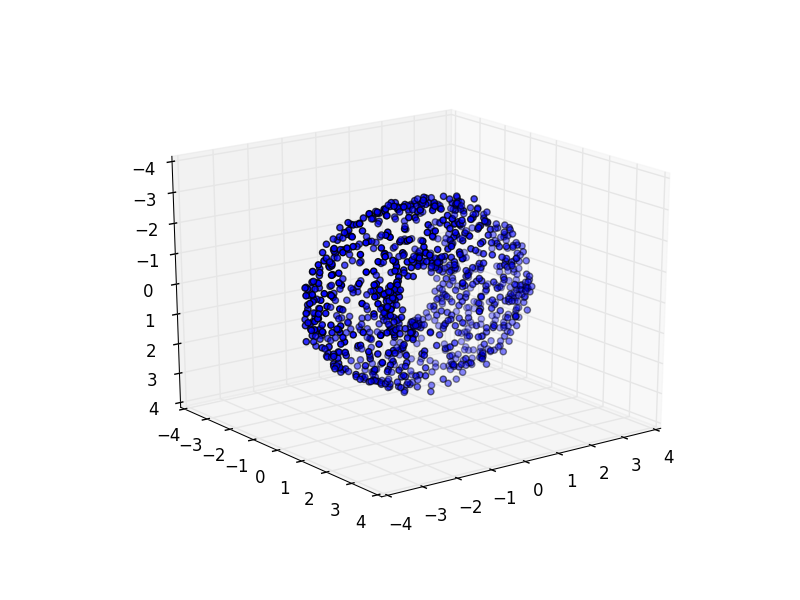
\includegraphics[scale=0.55]{img/t2.png}
\caption{Nube generada con \texttt{Cubix} en forma de $T^2$.}
\label{t2}
\end{figure}

Para hacer el cálculo de homología persistente basta con la siguiente instrucción:
\begin{lstlisting}[language=python]
  >> h = X.persistent_homology()
\end{lstlisting}

Como es evidente, si se ejecuta de esta forma tomará valores por defecto. Los argumentos que acepta el método \texttt{persistent\_homology()} son los siguientes:
\begin{itemize}
\item \texttt{n}: precisión de la cuadrícula. En concreto, es el número de puntos que tendrá la cuadrícula en cada dirección de $\R^n$. Valor por defecto: \texttt{10}.
\item \texttt{margin}: margen de la cuadrícula sobre los datos. Un valor \texttt{margin=0} montaría la cuadrícula más pequeña que contiene los datos en \texttt{X}, mientras que un valor \texttt{margin=0.1} daría un margen del 10\%. Valor por defecto: \texttt{0.1}
\item \texttt{pruning}: parámetro de poda. Se utiliza para mejorar el rendimiento. Si \texttt{pruning=0.9}, se prescinde de los cubos del complejo cúbico cuyo valor en el KDE sea mayor a 0.9 \footnote{Recordamos que \texttt{Cubix} escala las filtraciones para ir de 0 a 1, un valor próximo a 1 es por tanto un valor bajo en el KDE, son lugares donde la concentración de puntos es menospreciable.}. Si \texttt{pruning=0}, no se realiza poda. Valor por defecto: \texttt{0}.
\item \texttt{verbose}: variable booleana para imprimir por pantalla el progreso del cálculo. Resulta útil cuando se toman precisiones altas y el cálculo es lento. Valor por defecto: \texttt{False}.
\end{itemize}

Cuando se ha ejecutado la instrucción anterior, se tiene un objeto \texttt{h} que es de la clase \texttt{PersistentHomology} del módulo. Esta clase cuenta con 3 métodos para mostrar los resultados:
\begin{lstlisting}[language=python]
  >> h.persistence_diagram() # Diagrama de persistencia
  >> h.bar_code()            # Codigo de barras
  >> h.detail()              # Imprime por pantalla
\end{lstlisting}
La última nos enseña por pantalla los instantes de nacimiento y muerte (y la vida) de cada generador de persistencia de la filtración agrupados por dimensiones. Las dos primeras realizan un gráfico. En ambas, por defecto, se grafican los generadores de persistencia de todas las dimensiones utilizando distintos colores. Si se desea, pueden imprimirse sólo aquellas dimensiones que uno crea conveniente con el argumento \texttt{dimensions} (véase documentación). En la Figura \ref{plots} se muestran el diagrama de persistencia y el código de barras de una nube de datos con forma de $S^2$, realiados con \texttt{Cubix}.

\begin{figure}[h!]
\centering
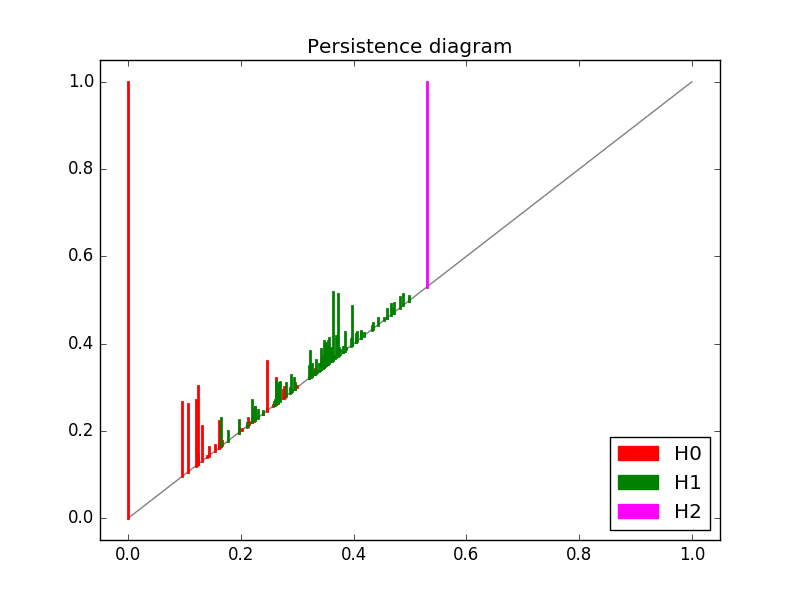
\includegraphics[scale=0.30]{img/s2diagram.png}
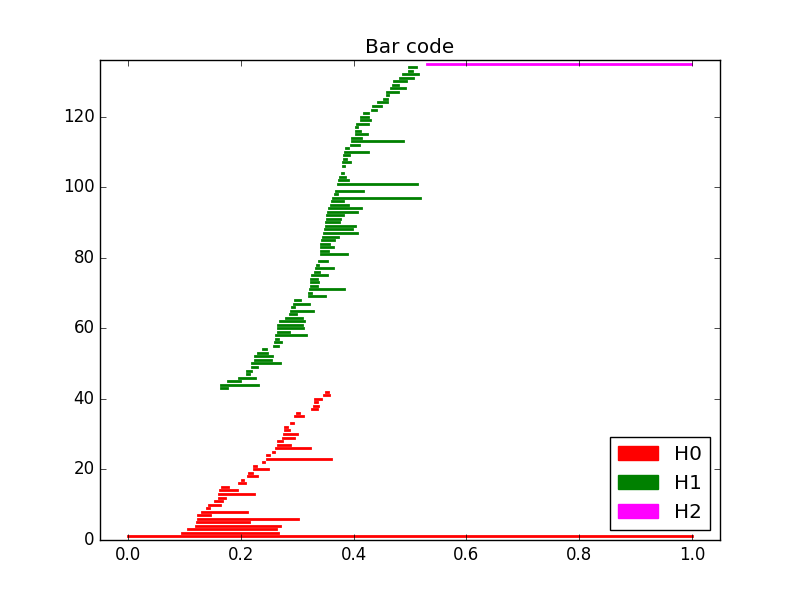
\includegraphics[scale=0.30]{img/s2barcode.png}
\caption{Diagrama de persistencia y código de barras con \texttt{Cubix}.}
\label{plots}
\end{figure}

\subsection{Algoritmo de cálculo de homología persistente}

El complejo cúbico sobre el que se construye la filtración es finito, lo cual hace que la filtración conste en un número finito de pasos, cada uno de los cuáles tiene un complejo cúbico finito. El álgebra lineal nos da un método para resolver el problema en un número finito de pasos, escalonando las matrices de los morfismos diferenciales del complejo $Q_*(K)$ para cada elemento $K$ de la filtración. Claro que sólo un complejo como el de la Figura \ref{grid} tiene 100 $0$-cubos (puntos), 180 $1$-cubos (aristas) y 81 $2$-cubos (cuadrados), con lo cual la matriz del morfismo $\partial_1$, por ejemplo, ya tiene dimensiones $181 \times 100$. A poco que uno quisiera aumentar la precisión de la cuadrícula o la dimensión del espacio el problema se convierte en algo computacionalmente inalcanzable si se realiza de este modo.

Es este apartado describiremos los pasos que sigue el algoritmo implementado en \texttt{Cubix} para el cálculo de generadores de persistencia, a partir de una nube de datos \texttt{X} de la clase \texttt{Cloud}.

\begin{enumerate}[(i)]
\item Se construye la cuadrícula sobre \texttt{X}. Se tiene la clase \texttt{Grid} que, dados los parámetros \texttt{n} y \texttt{margin}, calcula la posición de los puntos de la cuadrícula.

\item Se evalúa el KDE de la nube (\texttt{Cloud.kde}) en cada uno de los puntos de dicha cuadrícula. Se calcula aquí el valor máximo del KDE en la cuadrícula para después escalar.

\item Se construye el complejo cúbico sobre el que definir la filtración. Por cada punto de la cuadrícula y cada conjunto de direcciones posibles, se crea un cubo de la clase \texttt{Cube}.

\item A cada cubo se le asigna un valor de forma inductiva. Si se trata de un $0$-cubo, se le da el valor $1-v/m$ siendo $v$ el valor del punto correspondiente en el KDE, y $m$ el valor máximo del KDE \footnote{Aplicamos esta fórmula para escalar, y que los puntos con un valor más alto en el KDE sean próximos al 0, y los que tienen valor más bajo sea próximos al 1}. Si se trata de un $m$-cubo con $m>0$ entonces se le asigna como valor el máximo entre el valor de cada una de sus caras. Para calcular dichas caras, se cuenta con un método en la clase \texttt{Cube} que sigue la definición dada en la Sección 3.

\item Se ordenan en ascendentemente los cubos del complejo cúbico según el valor asignado y ---como segunda prioridad--- dimensión también ascendente. La lista ordenada de cubos se guarda en un objeto de la clase \texttt{Filtration}, la cual contiene el método \texttt{prune} para podar el complejo cúbico en caso de ser requerido.

\item Se pasa el objeto de la clase \texttt{Filtration} como argumento al constructor de la clase \texttt{PersistentHomology} y comienza el cálculo de los generadores persistentes de homología. Para este cálculo se asigna a cada cubo una \emph{clase} de homología (clase \texttt{HomologyClass}), que se tratan esencialmente como una lista de elementos no repetidos de generadores (clase \texttt{HomologyGenerator}). Por ello \texttt{Cubix} trabaja con $\F_2$: en una clase de homología, los generadores o están (que sería coeficiente 1) o no están (coeficiente 0). La suma de dos clases de homología es la diferencia simétrica de ambas clases, i.e., los generadores que están en una o en otra, pero no en ambas (si está en las dos se cancela).

El cálculo de los generadores de homología persistente consiste en el siguiente bucle:
\begin{itemize}
\item Por cada $m$-cubo de la filtración (recuérdese, ordenados por valor y dimensión), se calcula la \emph{diferencial} del cubo como la suma de las clases de homología de cada una de sus caras. En función de esta diferencial se procede de alguna de las siguientes formas:

\begin{itemize}
\item Si la diferencial es 0 entonces el cubo es un nuevo generador de homología ya que no puede ser frontera de un $m+1$-cubo porque el valor del $m+1$-cubo es el máximo del valor de sus caras y tiene dimensión superior, con lo cual aparece más adelante en la filtración. Se crea en este caso un elemento $g$ de la clase \texttt{HomologyGenerator} al que se le indica como instante de nacimiento el valor del $m$-cubo que lo ha generado, y se asigna al $m$-cubo la clase $\{ g \}$.

\item Si la diferencial es diferente de 0, entonces se tiene que esta suma de generadores en dimensión $m-1$ de la forma
$$ g_1 + g_2 + ... + g_r $$
es ahora imagen de un $m$-cubo, y por tanto pasa a ser 0 en este punto de la filtración. Como se trabaja en $\F_2$, podemos despejar uno de los generadores y escribirlo en función de los otros. Se toma de entre los generadores que aparecen en la suma el más joven (punto de nacimiento mayor), supongamos $g_1$, y se escribe como suma de los otros. En todas las clases de homología que se tengan en este momento de la filtración, se sustituye (donde aparezca) el generador $g_1$ y por la suma $g_2+\dots+g_r$. En este momento decimos que muere el generador $g_1$ y le asignamos como instante de muerte el valor del $m$-cubo del paso. Al $m$-cubo se le pone como clase de homología la clase 0.
\end{itemize}
\end{itemize}

Nótese que en particular puede haber generadores que nacen y mueren en el mismo instante, ya que con el mismo valor que lo genera un $m$-cubo puede venir después un $m+1$ cubo que lo mate. Se almacenan en la clase \texttt{PersistentHomology} una lista con todos los generadores que han aparecido y que han tenido vida (que no mueren en el mismo instante que nacen). Estos valores de nacimiento y muerte son los que se utilizan en los métodos de representación de la clase: \texttt{detail}, \texttt{persistence\_diagram} y \texttt{barcode}.

\end{enumerate}


\subsection{KDE utilizado}
No es objeto de este trabajo entrar en el debate de qué kernel o qué bandwidth estima mejor la nube de datos. Para el desarrollo en Python de nuestro método se ha utilizado el KDE Gaussiano, el cual ya está implementado en la librería \texttt{scipy} con la clase \texttt{scipy.stats.gaussian\_kde}.

El KDE Gaussiano entiende cada punto del espacio $\R^n$ como desviaciones de varianza $h^2$ de los puntos de la muestra. Así, la función kernel no es más que la densidad de una normal estándar y el resultado del estimador de densidad es el siguiente:

$$ \hat{f}_h(x) = \frac{1}{N} \sum_{i=1}^{N} \frac{1}{h^n}\frac{1}{\sqrt{2\pi}}e^{-\frac{\Vert x - x_i \Vert ^2}{h^2\sqrt{2\pi}}} $$

El kernel de Gauss es ampliamente usado dada su sencillez. Tiene una eficiencia del 95.1\% con respecto al kernel de Epanechnikov \cite{Scheid}, que es el que minimiza el error cuadrático medio.

El bandwidth utilizado por defecto en el KDE Gaussiano de la librería \texttt{scipy} se calcula a través de la regla de Scott
$$ h_S = N^{-\frac{1}{n+4}} $$
donde, recordemos, $N$ es el número de puntos y $n$ la dimensión del espacio ambiente. Para más información sobre la regla de Scott redirigimos a \cite{Scott}.

En el módulo \texttt{Cubix}, el KDE se define automáticamente al instanciar la clase \texttt{Cloud} en el campo \texttt{kde} usando los valores por defecto de la función \texttt{scipy.stats.gaussian\_kde}, y por tanto con el bandwidth dado por la regla de Scott. Uno puede cambiar el ancho de banda de un objeto \texttt{X} de la clase \texttt{Cloud} utilizado con la instrucción:
\begin{lstlisting}[language=python]
  >> X.kde.set_bandwidth(bw_method=scalar)
\end{lstlisting}
donde \texttt{scalar} puede ser el número que uno desee. Para más información, véase la documentación de dicha función en https://docs.scipy.org/.

%\subsection{\texttt{Cubix} vs. \texttt{Dionysus}}



\newpage
\NewPage
\section{Conclusiones}

% --------------------------------
%
% SECCIÓN 6: CONCLUSIONES
%
% --------------------------------

Las filtraciones mediante KDE nos proporcionan un método alternativo para estimar grupos de homología, y además aportan un punto de vista muy diferente a la homología persistente mediante Vietoris-Rips. Se destacan dos características principales:

\begin{itemize}
\item \textbf{Robustez frente a ruidos}. Cuánto más alto es el número de puntos, mayor es el contraste de la función kernel y por ello más insignificantes se vuelven los puntos donde la concentración es baja, posicionando estos puntos lejos en la filtración.
\item \textbf{Elección de la precisión}. Con este tipo de filtraciones, uno puede elegir la precisión de la cuadrícula. Si se toman $n$ puntos en cada dirección del espacio $\R^m$, el número de cubos simpliciales del complejo sobre el que se filtra es $(2n-1)^m$, que no depende del número de datos $N$. Esto difiere de la filtración de Vietoris-Rips, donde el número de símplices del complejo cúbico es $2^N$. Este hecho permite reducir considerablemente el tiempo de computación.
\end{itemize}

Sin duda, quedan muchos frentes abiertos en los que avanzar en este tema. A continuación se exponen algunos puntos que sería interesante tratar en un futuro:
\begin{itemize}
\item \textbf{Eficiencia computacional}. Aun a pesar de las ventajas que pueda tener el método de filtraciones por KDE's, el módulo \texttt{Cubix} no puede hacer frente computacionalmente a librerías como \texttt{PHAT}, \texttt{Dionysus} o \texttt{TDA}. Evidentemente, le pasa factura el estar desarrollado en un lenguaje de programación interpretado. Pese a que el objetivo principal era desarrollar un módulo 100\% escrito en Python ---al ver que no existía ninguno---, salta a la vista que ante algoritmos con altos requerimientos es preferible hacerlo en un lenguaje compilado y crear luego \emph{bindings} (enlaces), como hace \texttt{Dionysus}.

\item \textbf{Dependencia del número de datos}. Cierto es que el número de cubos de la filtración no depende del número de datos, pero no es verdad que el tiempo de computación no dependa de ello. En efecto, de la forma que funciona \texttt{gaussian\_kde()} de \texttt{scipy}, se utiliza cada uno de los puntos cada vez que se evalúa el KDE. Así pues, al aumentar el número de datos aumenta el tiempo que tarda no en calcular los generadores de persistencia, pero sí (y considerablemente) en evaluar el KDE en los puntos de la cuadrícula. Una buena solución a este problema sería \emph{suavizar} antes el KDE (interpolando, por ejemplo) para quedarnos con un polinomio para evaluar. Sobre este tema de \emph{suavizar} el KDE habla Scheid en \cite{Scheid} y resultaría interesante aplicarlo.

\item \textbf{Detectar grupos de torsión}. Como ya hemos dicho, \texttt{Cubix} ---al igual que la mayoría de software relacionado--- trabaja con coeficientes en $\F_2$. Al tratarse de un cuerpo, nunca se obtendrán grupos de torsión, sólo un número de copias de dicho cuerpo. Ésto significa que, por ejemplo, no podremos diferenciar un plano proyectivo $\RP^2$ de un objeto contráctil. El motivo de que se haya utilizado $\F_2$ tiene que ver con el hecho de cómo funciona el algoritmo de cálculo, ya que en un momento dado necesitamos despejar un elemento de una suma (véase Sección 5). No se me ocurrió una alternativa para hacer un procedimiento igualmente eficiente que no requiera de un cuerpo para los $R$-módulos. Un avance en esta dirección sería un gran paso.

\item \textbf{Elección del KDE}. Sin duda, la elección del KDE y el \emph{bandwidth} es fundamental y aporta resultados tremendamente distintos al variar uno u otro. Debería profundizarse mucho más sobre qué elegir y cuál es el criterio a seguir.

\item \textbf{Filtraciones para funciones}. La filtración en complejo cúbico no se construye directamente a partir de una nube de datos, sino a partir de una función. Esta forma de proceder permitiría hablar de generadores de persistencia de cualquier función $\map{f}{\R^m}{\R}$, sin necesidad de considerar una nube de datos de la cual es KDE. \emph{¿Podemos definir la forma de una función?}.

\end{itemize}

\newpage
\begin{thebibliography}{99}
\bibitem{Atiyah}
M. Atiyah, I. Macdonald (1969) \\
``Introduction to Commutative Algebra'' \\
http://www.saheleriyaziyat.net/images/k1zut2e5peefixbx6kty.pdf

\bibitem{Bjorner}
A. Björner (2002) \\
``Nerves, fibers and homotopy groups'' \\
http://www.maths.ed.ac.uk/~v1ranick/papers/bjorner1.pdf

\bibitem{Carlsson}
G. Carlsson, A. Zomorodian, A. Collins, L. Guibas (2005) \\
``Persistence barcodes for shapes'' \\
http://citeseerx.ist.psu.edu/viewdoc/download?doi=10.1.1.5.2718 \\
\&rep=rep1\&type=pdf

\bibitem{Chouaib}
A. Chouaib (2015) \\
\small
``Kernel Estimator and Bandwidth Selection for Density and its Derivatives'' \\
\normalsize
https://cran.r-project.org/web/packages/kedd/vignettes/kedd.pdf

\bibitem{Edelsbrunner}
H. Edelsbrunner, D. Letscher, A. Zomorodian (2002) \\
``Topological Persistence and Simplification'' \\
http://www.math.uchicago.edu/\textasciitilde shmuel/AAT-readings/Data Analysis /Edelsbrunner-Letscher-Zomordian.pdf

\bibitem{Ghrist}
R. Ghrist (2008)\\
``Barcodes: The Persistent Topology of Data'' \\
https://www.math.upenn.edu/~ghrist/preprints/barcodes.pdf

\bibitem{Hatcher}
A. Hatcher (2001) \\
``Algebraic Topology'' \\
https://www.math.cornell.edu/~hatcher/AT/AT.pdf

\bibitem{Massey}
W. Massey (1991) \\
``A Basic Course in Algebraic Topology''

\bibitem{Navarro}
V. Navarro, P. Pascual (1999) \\
``Topologia Algebraica'' \\

\bibitem{Scheid}
S. Scheid (2004) \\
``Introduction to Kernel Smoothing'' \\
http://compdiag.molgen.mpg.de/docs/talk\_05\_01\_04\_stefanie.pdf

\bibitem{Scott}
D. Scott (1986) \\
\small
``Multivariate Density Estimation: Theory, Practice, and Visualization''
\normalsize

\end{thebibliography}

\NewPage
\end{document}
